\documentclass[a4paper,12pt]{book}
\usepackage[space]{ctex}
\usepackage{amsmath}
\usepackage{times}
\usepackage{titlesec}
\usepackage{titlesec}
\graphicspath{{./pic/chapter1/}{./pic/chapter2/}{./pic/chapter3/}}
\usepackage{graphicx}
\usepackage{float}
\usepackage{pythonhighlight}
\usepackage{caption}
\usepackage{subfigure}
\titleformat
{\chapter} % command
[display] % shape
{\bfseries\Large\itshape} % format
{Tensorflow No. \ \thechapter} % label
{0.5ex} % sep
{\rule{\textwidth}{1pt}
\vspace{1ex}
\centering
}
[\vspace{-0.5ex}%
\rule{\textwidth}{0.3pt}
] % after-code
\begin{document}
\date{\today}
\tableofcontents
\newpage
\chapter{Tensorflow基础}
\section{Tensorflow基础函数}
\subsection{Variable}
\begin{python}
#tensorflow 1.2.1
import tensorflow as tf
var = tf.Variable(0)
add_operation = tf.add(var,1)
update_operation = tf.assign(var,add_operation)
with tf.Session() as sess:
    sess.run(tf.global_variables_initializer())
    for _ in range(3):
        sess.run(update_operation)
        print(sess.run(var))
\end{python}
\subsection{placeholder}
\begin{python}
#tensorflow 1.2
import tensorflow as tf
x1 = tf.placeholder(dtype=tf.float32,shape=None)
y1 = tf.placeholder(dtype=tf.float32,shape=None)
z1 = x1+y1
x2 = tf.placeholder(dtype=tf.float32,shape=[2,1])
y2 = tf.placeholder(dtype=tf.float32,shape=[1,2])
z2 = tf.matmul(x2,y2)
with tf.Session() as sess:
    z1_value = sess.run(z1,feed_dict={x1:1,y1:2})
    z1_value,z2_value = sess.run([z1,z2],feed_dict={x1:1,y1:2,x2:[[2],[2]],y2:[[3,3]]})
    print(z1_value)
    print(z2_value)
\end{python}
\subsection{batch normalization}

\begin{itemize}
	\item[\S] 数据x为Tensor。
\item mean:为x的均值,也是一个Tensor。
\item var:为x的方差,也为一个Tensor。
\item offset:一个偏移,也是一个Tensor。
\item scale:缩放倍数,也是一个Tensor。
\item variable\_epsilon,一个不为0的浮点数。
\item name:操作的名字,可选。
\end{itemize}
batch normalization计算方式是:
\begin{gather}
x = (x-\bar{x})/\sqrt{Var(x)+variable_{epsilon}}\\
x = x\times scale+offset\\
\end{gather}
\begin{gather}
\text{均值}:\bar{x} = \frac{1}{m}\Sigma_{i=1}^{m}x_i\\
\text{方差}:\sigma^2 = \frac{1}{m}\Sigma_{i=1}^m(x_i-\bar{x})
\end{gather}
\section{常见的激活函数}
\subsection{relu}
relu函数在自变量x小于0时值全为0,在x大于0时,值和自变量相等。
\begin{python}
import tensorflow as tf 
import matplotlib.pyplot as plt 
x = tf.linspace(-10.,10.,100)
y = tf.nn.relu(x)
with tf.Session() as sess:
	[x,y] = sess.run([x,y])
plt.plot(x,y,'r',6,6,'bo')
plt.title('relu')
ax = plt.gca()
ax.annotate("",
            xy=(6, 6), xycoords='data',
            xytext=(6, 4.5), textcoords='data',
            arrowprops=dict(arrowstyle="->",
                            connectionstyle="arc3"),
            )
ax.annotate("",xy=(6,6),xycoords='data',
            xytext=(10, 6), textcoords='data',
            arrowprops=dict(arrowstyle="->",
                            connectionstyle="arc3"),
	  	   
)
ax.grid(True)
plt.xlabel('x')
plt.ylabel('relu(x)')
plt.savefig('relu.png',dpi = 600)
\end{python}
\subsection{relu6}
relu6函数和relu不同之处在于在x大于等于6的部分值保持为6。
\begin{python}
import tensorflow as tf 
import matplotlib.pyplot as plt 
x = tf.linspace(-10.,10.,100)
y = tf.nn.relu6(x)
with tf.Session() as sess:
	[x,y] = sess.run([x,y])
plt.plot(x,y,'r',6,6,'bo')
plt.title('relu6')
ax = plt.gca()
ax.annotate("",
            xy=(6, 6), xycoords='data',
            xytext=(6, 4.5), textcoords='data',
            arrowprops=dict(arrowstyle="->",
                            connectionstyle="arc3"),
            )
ax.grid(True)
plt.xlabel('x')
plt.ylabel('relu6(x)')
plt.savefig('relu6.png',dpi = 600)
\end{python}
\begin{figure}[H]
\centering
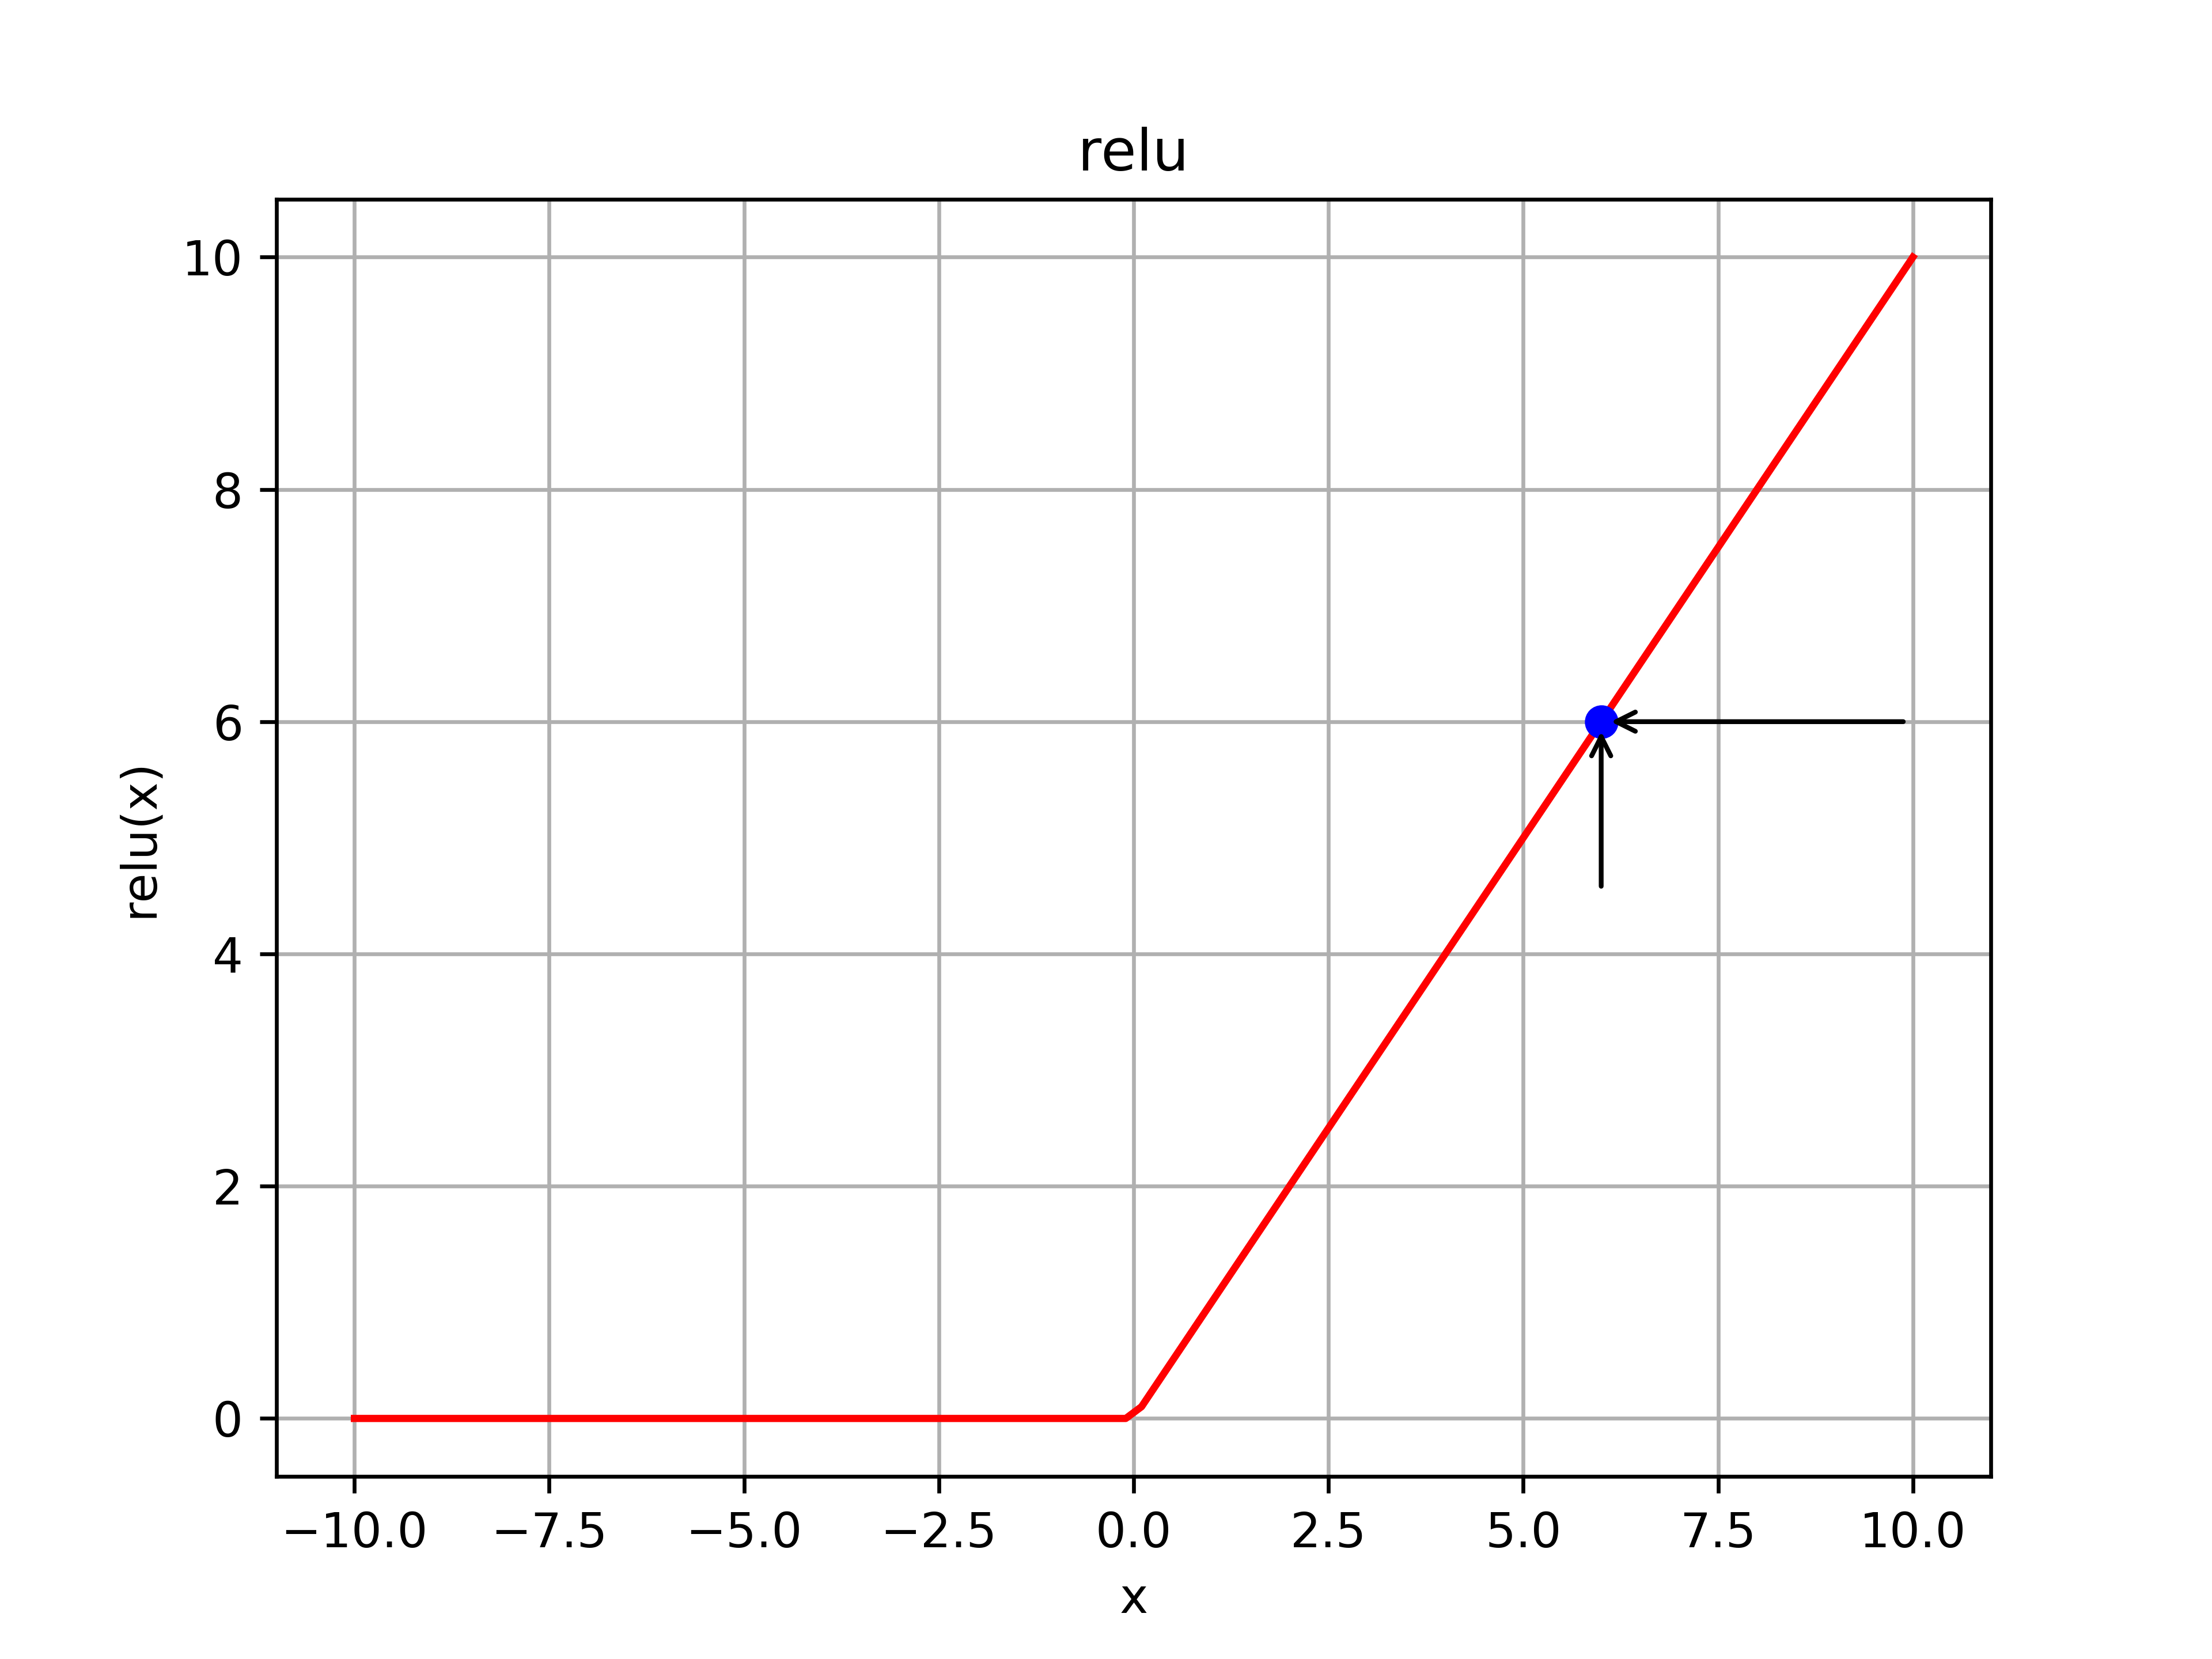
\includegraphics[scale=0.8]{./pic/chapter1/relu.png}
\caption{relu}
\end{figure}
\begin{figure}[H]
\centering
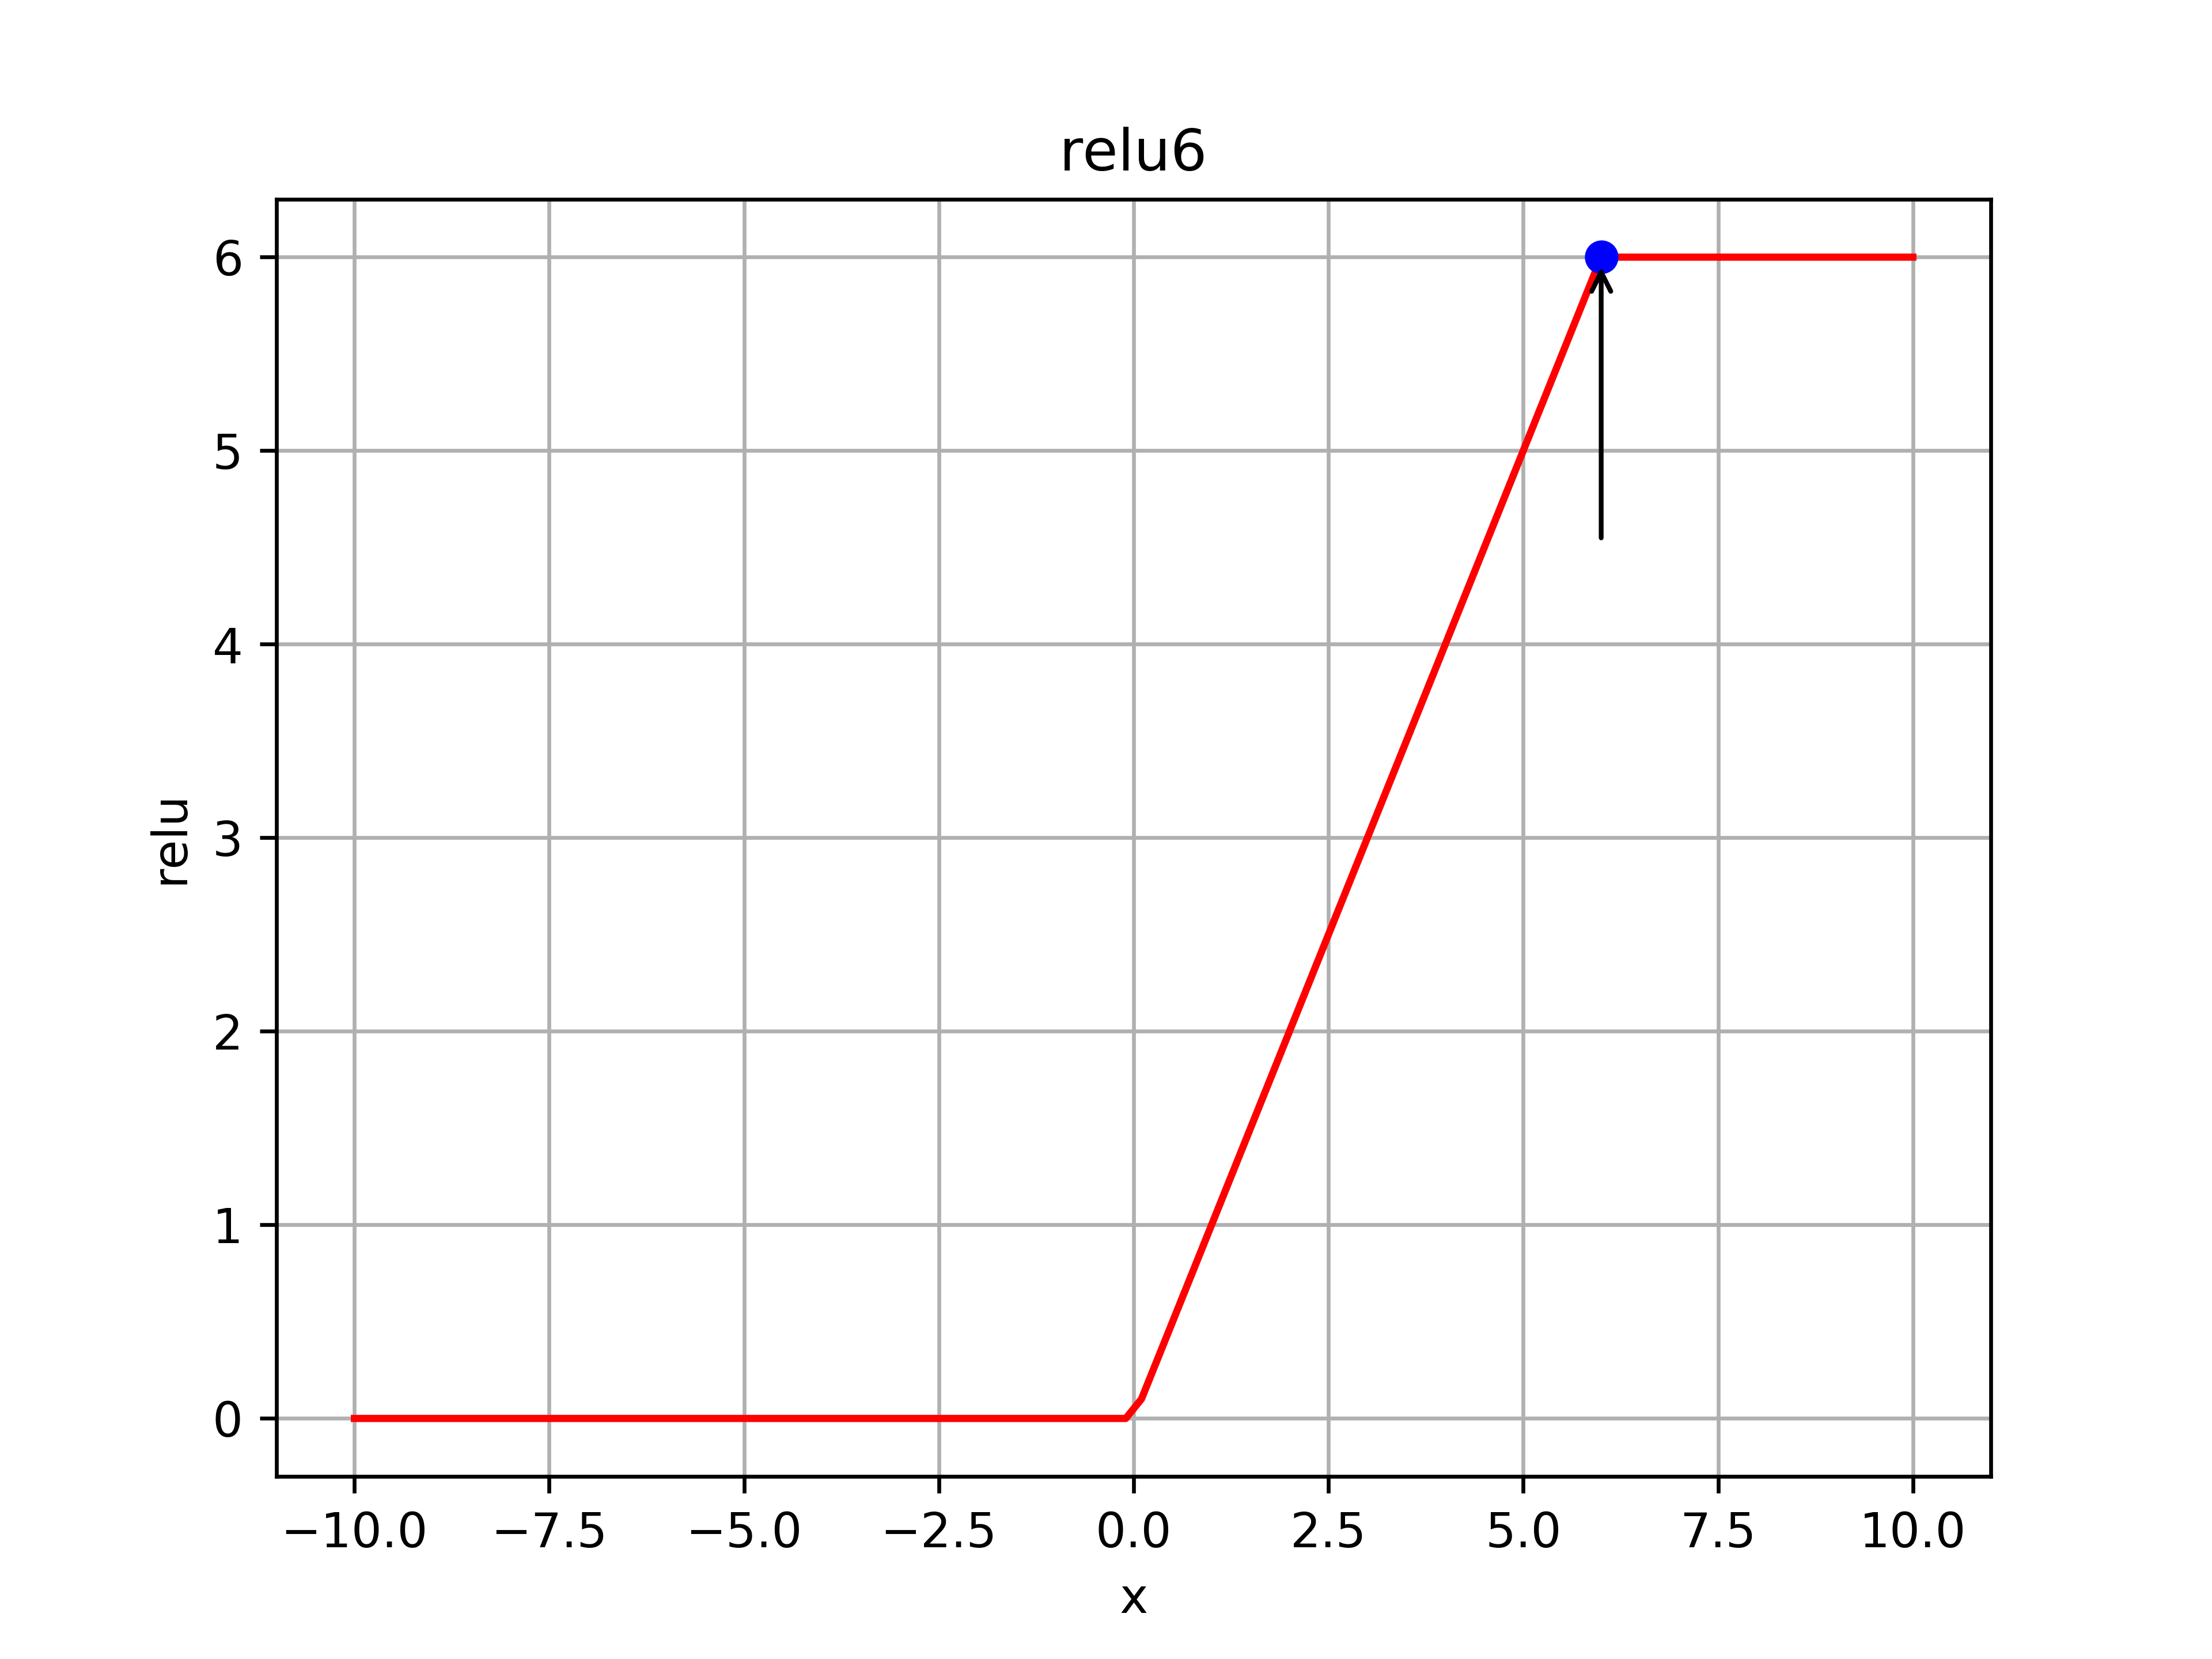
\includegraphics[scale=0.8]{./pic/chapter1/relu6.png}
\caption{relu6}
\end{figure}

\subsection{sigmoid}
\begin{python}
import tensorflow as tf 
import matplotlib.pyplot as plt 
import matplotlib.patches as mpatches
x = tf.linspace(-10.,10.,100)
y1 = tf.nn.sigmoid(x)
y2 = tf.nn.tanh(x)
red_patch = mpatches.Patch(color = 'red',label = 'sigmoid')
blue_patch = mpatches.Patch(color = 'blue',label = 'tanh')
with tf.Session() as sess:
	[x,y1,y2] = sess.run([x,y1,y2])
plt.plot(x,y1,'r',x,y2,'b')
ax = plt.gca()
ax.annotate(r"$tanh(x) = \frac{1-^{-2x}}{1+e^{-x}}$",
	   xy=(0,0),xycoords="data",
	   xytext=(1,0),textcoords="data",
	   arrowprops=dict(arrowstyle="->",
	   connectionstyle="arc3"),
)
ax.annotate(r"$sigmoid(x) = \frac{1}{1+e^{-x}}$",
	   xy=(0,0.5),xycoords="data",
	   xytext=(1,0.5),textcoords="data",
	   arrowprops=dict(arrowstyle="->",
	   connectionstyle="arc3"),
)
plt.xlabel('x')
plt.grid(True)
plt.legend(handles = [red\_patch,blue\_patch])
plt.savefig('activate.png',dpi=600)
\end{python}
\begin{figure}[H]
\centering
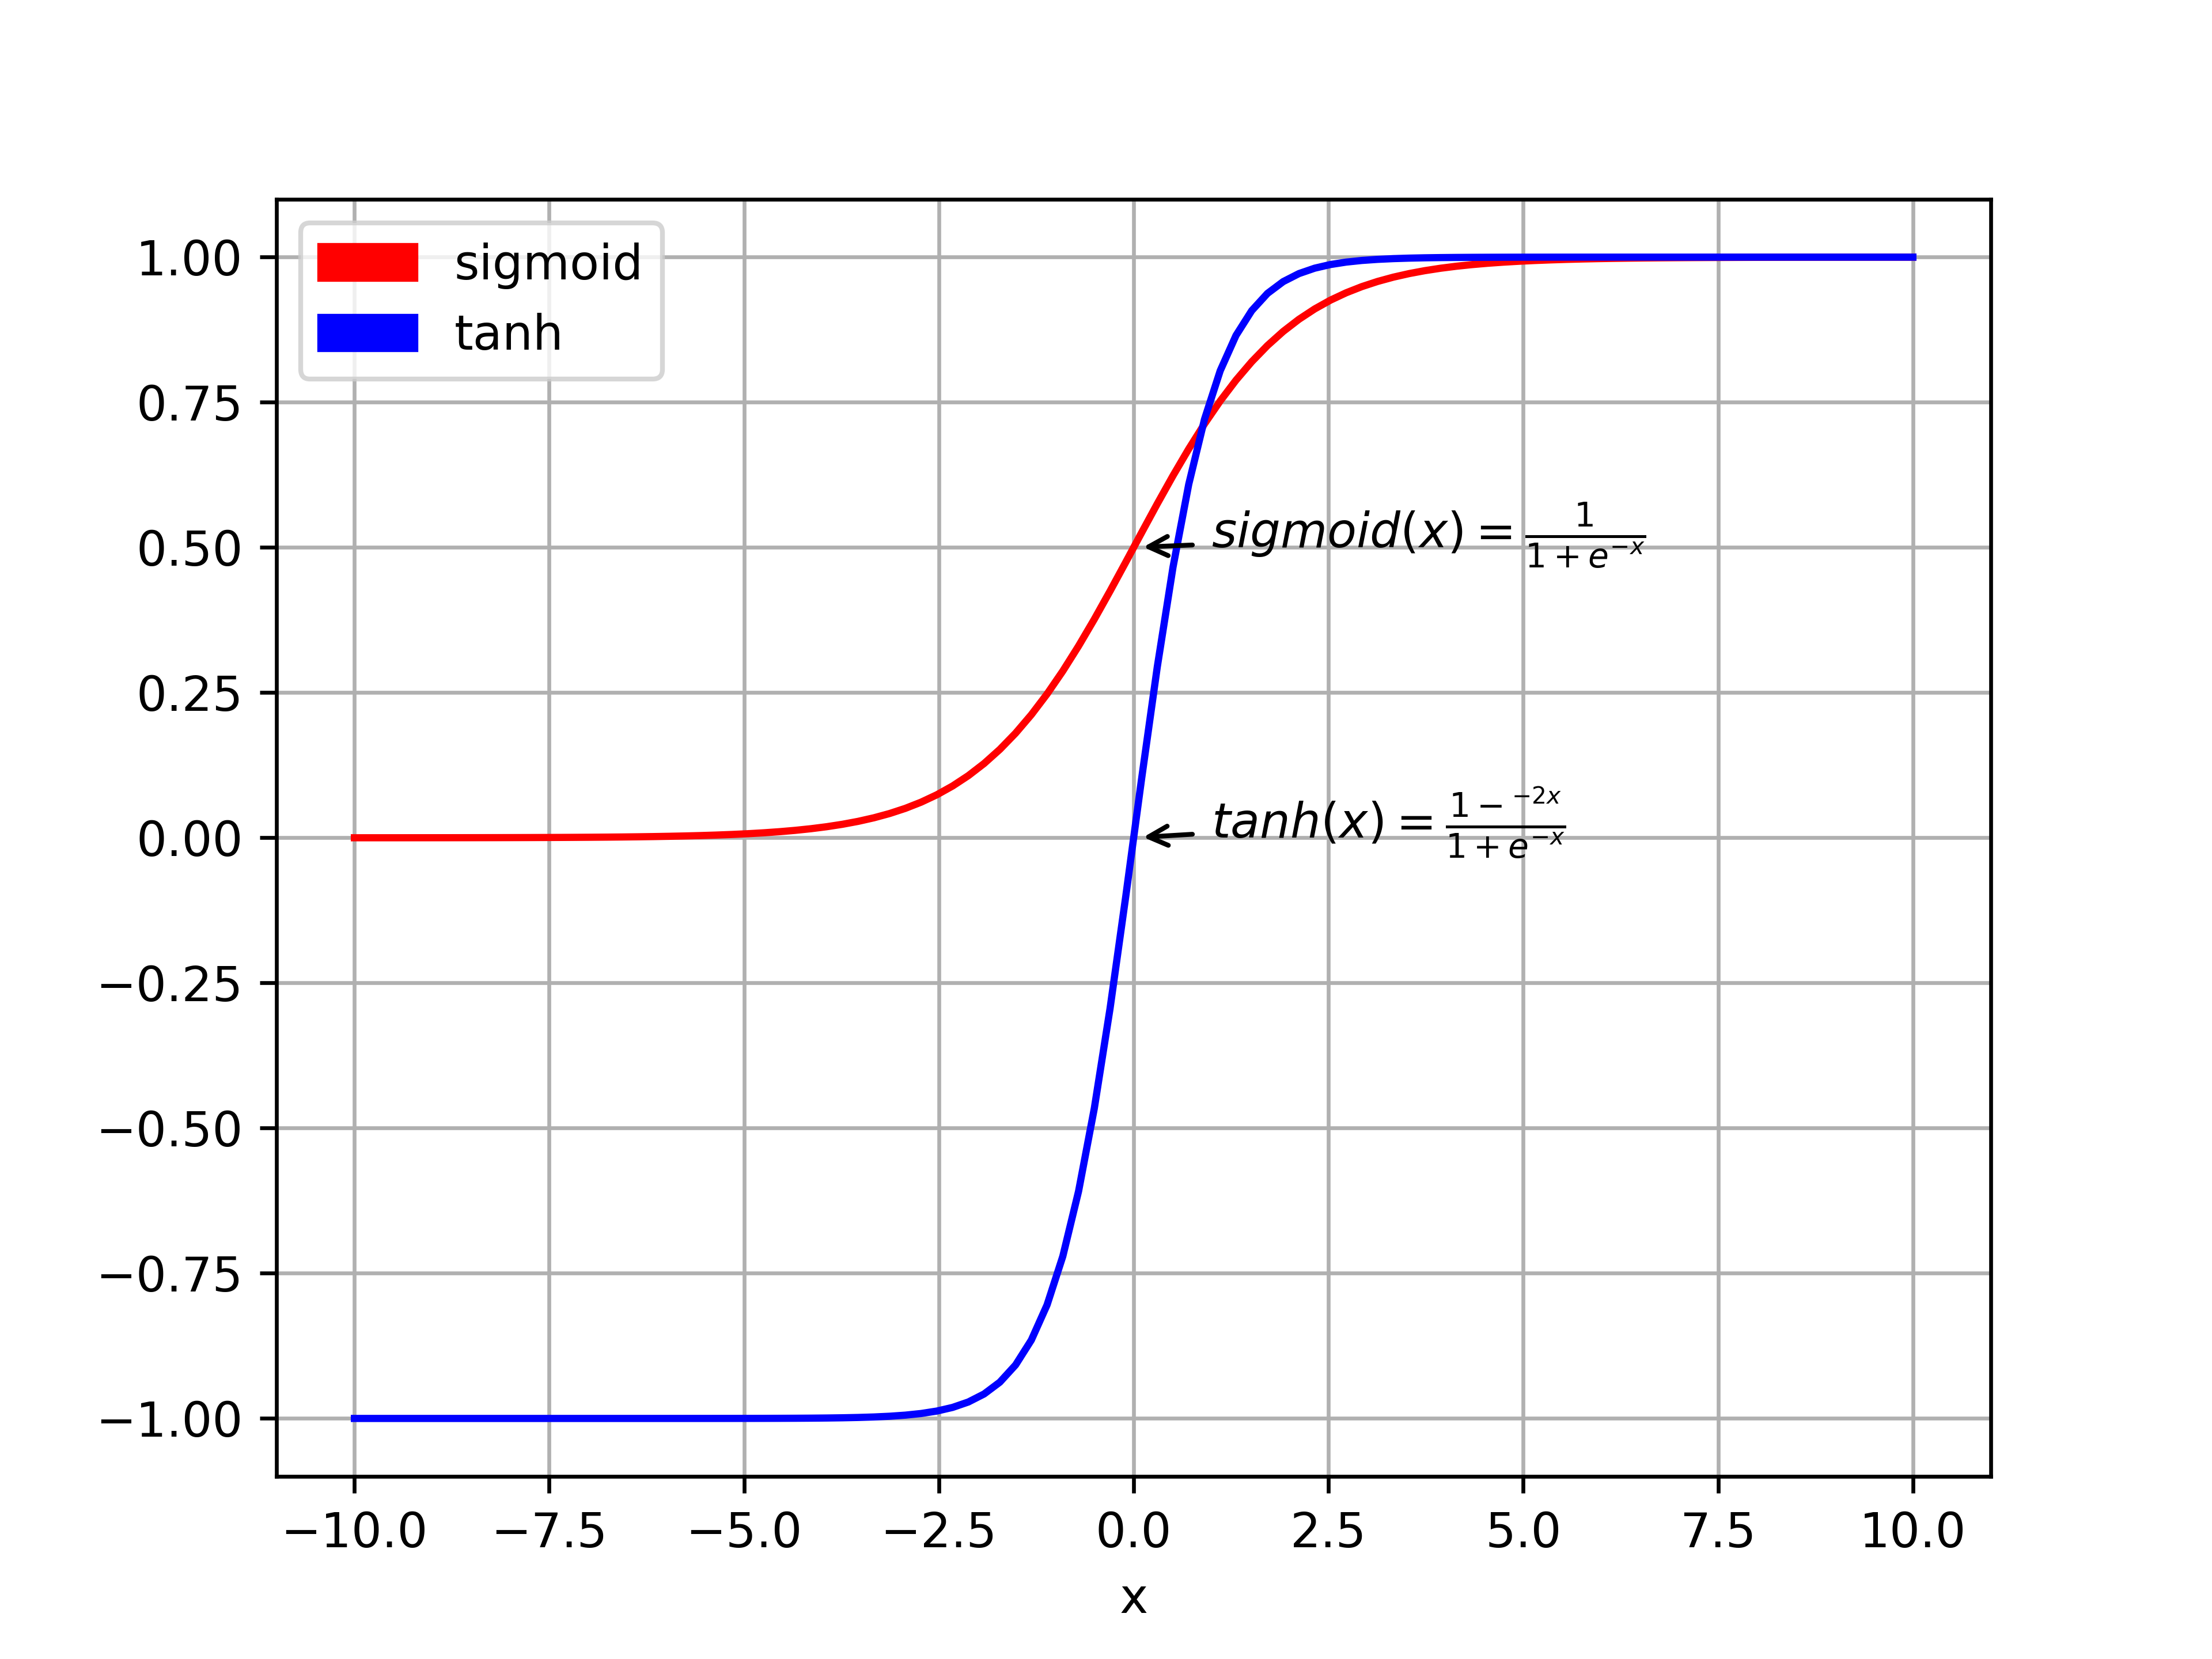
\includegraphics[scale=0.8]{./pic/chapter1/activate_fun.png}
\caption{activate\_fun}
\end{figure}
\subsection{relu和softplus}
\begin{python}
import tensorflow as tf 
import matplotlib.pyplot as plt 
import matplotlib.patches as mpatches
x = tf.linspace(-10.,10.,100)
y2 = tf.nn.softplus(x)
y3 = tf.nn.relu(x)
blue_patch = mpatches.Patch(color = 'blue',label = 'softplus')
yellow_patch = mpatches.Patch(color = 'yellow',label = 'relu')
with tf.Session() as sess:
	[x,y2,y3] = sess.run([x,y2,y3])
plt.plot(x,y2,'b',x,y3,'y')
ax = plt.gca()
plt.xlabel('x')
ax.annotate(r"$softplus(x)=log(1+e^x)$",
	   xy=(0,0),xycoords="data",
	   xytext=(1,0),textcoords="data",
	   arrowprops=dict(arrowstyle="->",
	   connectionstyle="arc3"),
)
ax.annotate(r"$relu(x)=max(x,0)$",
	   xy=(0,0.5),xycoords="data",
	   xytext=(1,0.5),textcoords="data",
	   arrowprops=dict(arrowstyle="->",
	   connectionstyle="arc3"),
)

plt.grid(True)
plt.legend(handles = [blue_patch,yellow_patch])
plt.savefig('relu_softplus.png',dpi=600)
\end{python}
\begin{figure}[H]
\centering
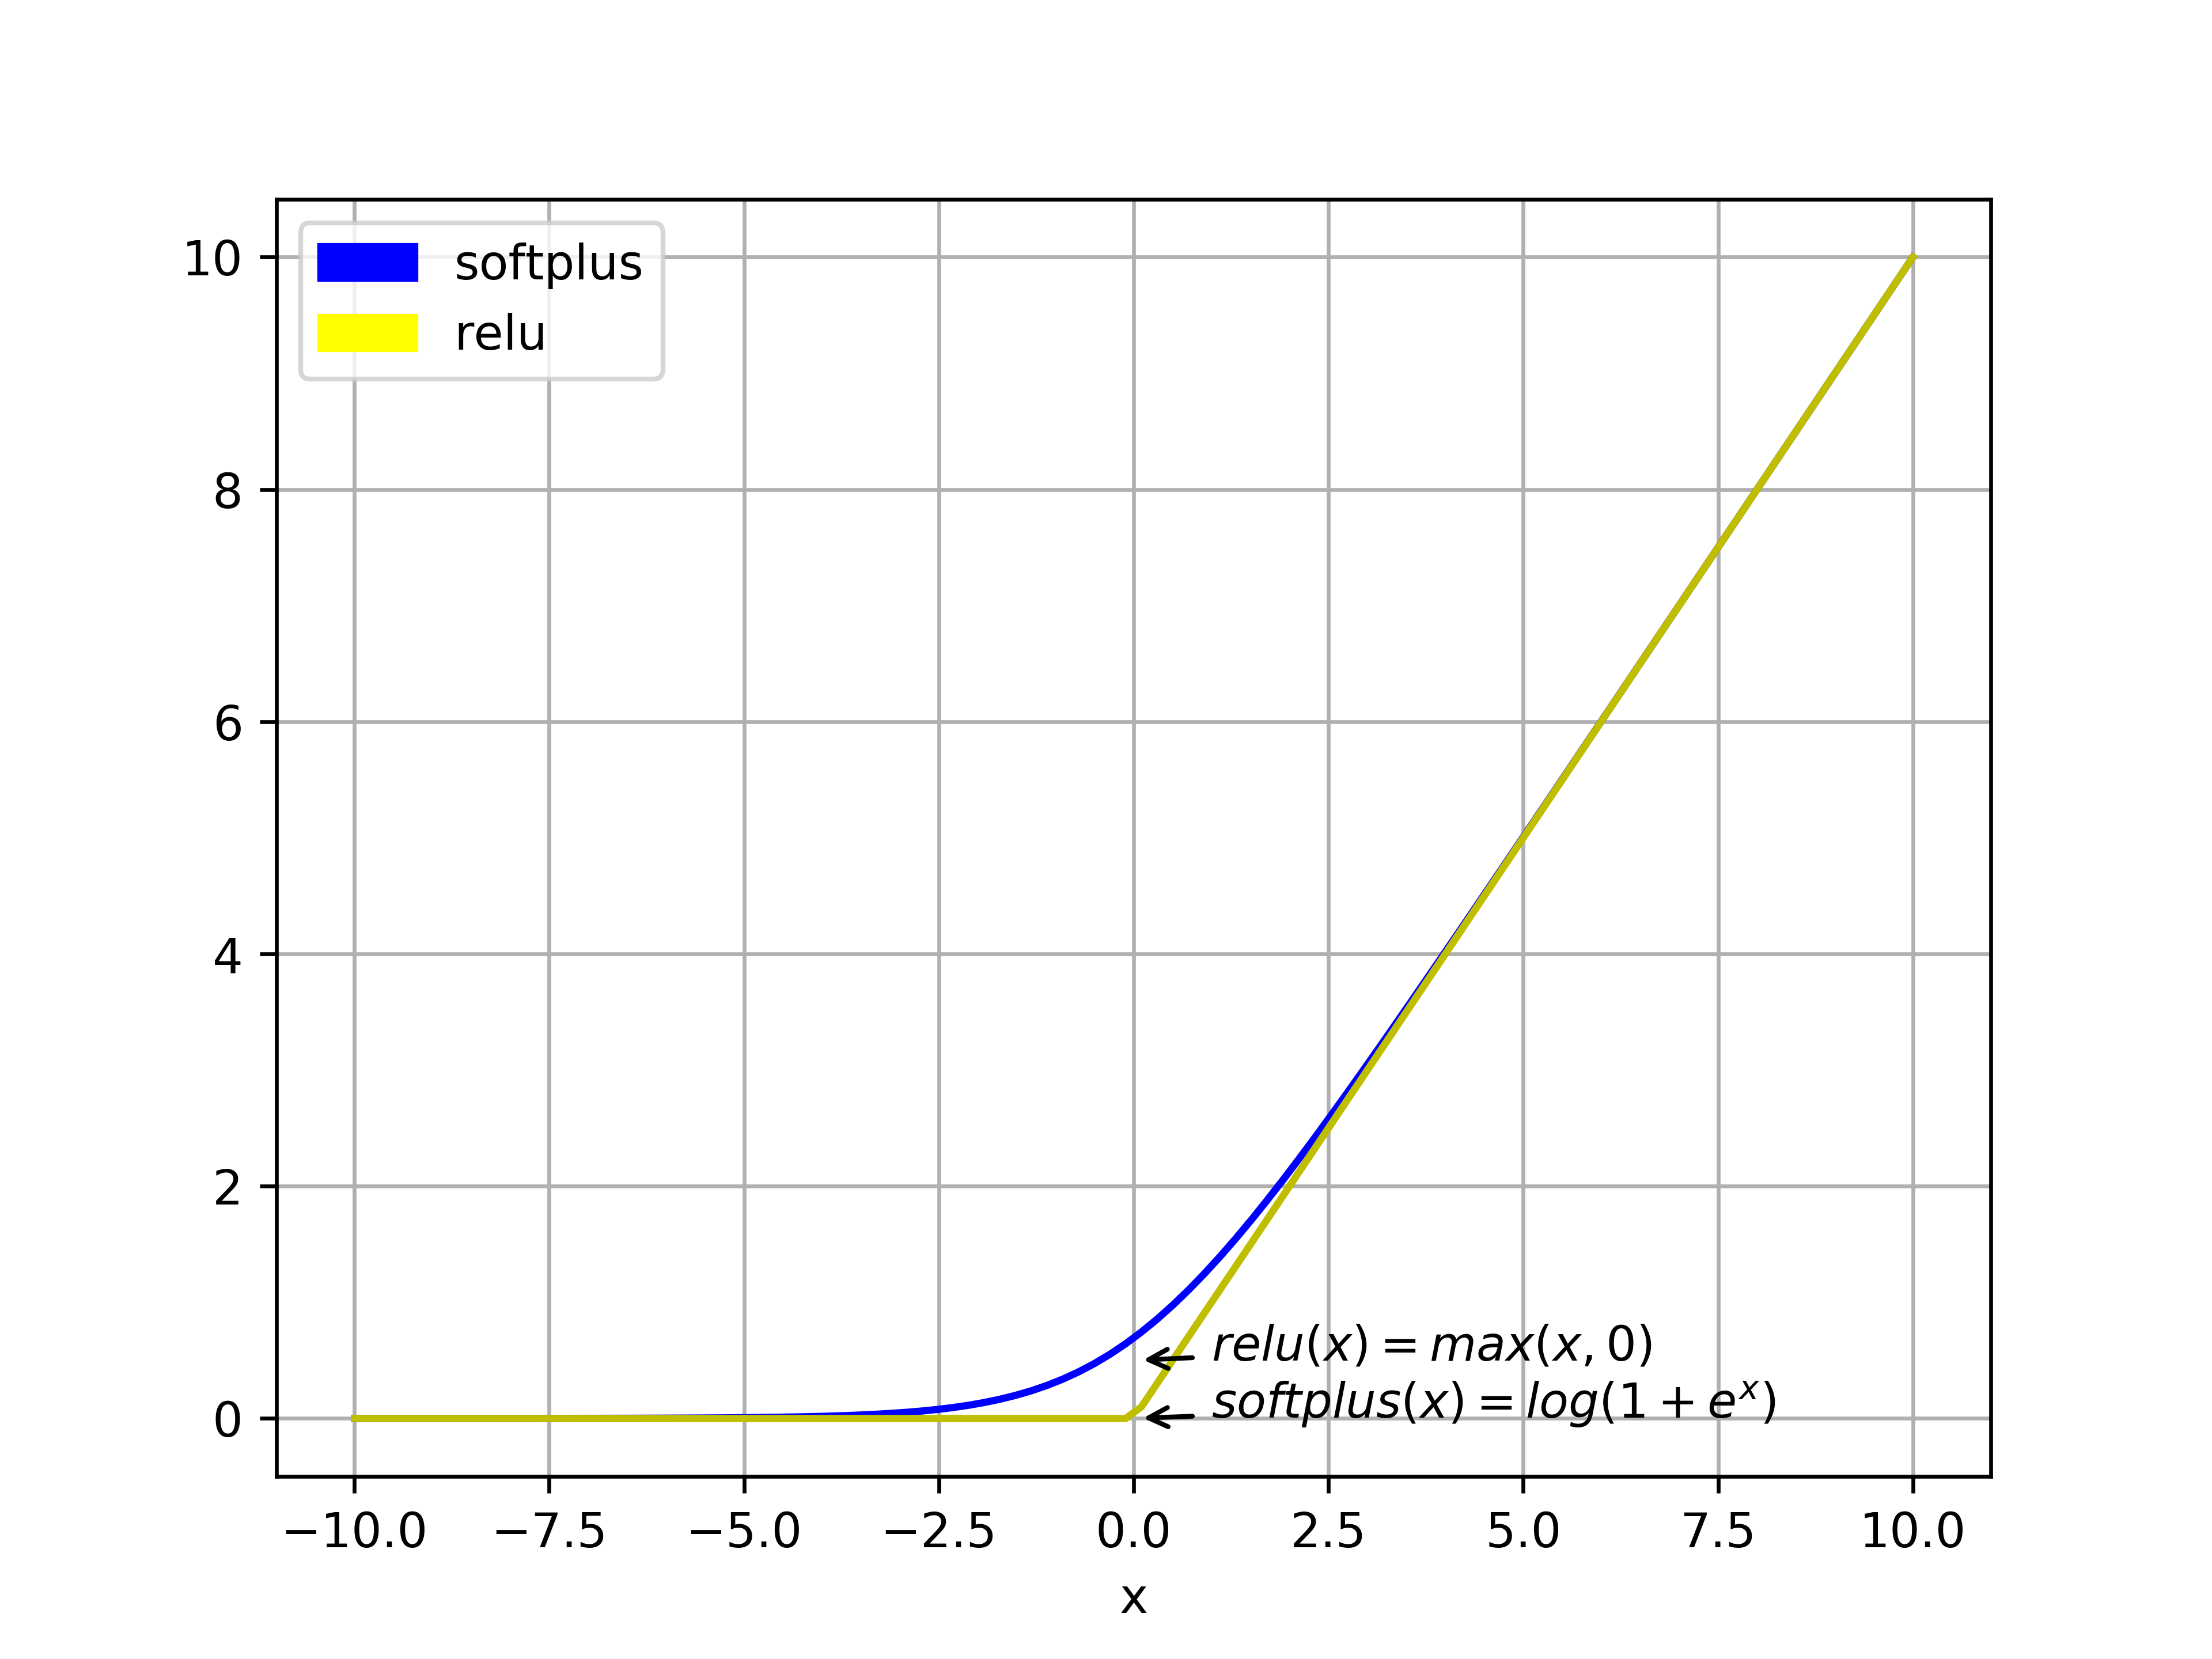
\includegraphics[scale=0.8]{./pic/chapter1/relu_softplus.png}
\end{figure}
\subsection{dropout}
将神经元以概率keep\_prob绝对是否被抑制。如果被抑制该神经元的输出为0如果不被抑制,该神经元的输出将被放大到原来的1/keep\_prop。
默认情况下,每个神经元是否被抑制是相互独立的。但是是否被抑制也可以通过noise\_shape来调节。当noise\_shape[i]=shape(x)[i]时,x中的元素相互独立。如果shape(x)=[k,1,1,n],那么每个批通道都是相互独立的,但是每行每列的数据都是关联的,也就是说要么都为0,要么还是原来的值。
\begin{python}
import tensorflow as tf
a = tf.constant([[-1.,2.,3.,4.]])
with tf.Session() as sess:
    b = tf.nn.dropout(a,0.5,noise_shape=[1,4])
    print(sess.run(b))
    c = tf.nn.dropout(a,0.5,noise_shape=[1,1])
    print(sess.run(c))
\end{python}
[[-2.  0.  0.  8.]]\newline
[[-0.  0.  0.  0.]]\newline
当输入数据特征相差明显时,用tanh效果会很好,但在循环过程中会不断扩大特征效果并显示出来。当特征相差不明显时,sigmoid效果比较好。同时,用sigmoid和tanh作为激活函数时,需要对输入进行规范化,否则激活厚的值全部进入平坦区,隐藏层的输出会趋同,丧失原来的特征表达,而relu会好很多,优势可以不需要输入规范化来避免上述情况。因此,现在大部分卷积神经网络都采用relu作为激活函数。
\section{CNN常用函数}
\subsection{卷积函数}
tf.nn.conv2d(input,filter,padding,stride=None,diation\_rate=Nonei每name = None,data\_format=None)\newline
\begin{itemize}
\item input:一个tensor,数据类型必须是float32,或者是float64
\item filter:一个tensor,数据类型必须和input相同。
\item strides:一个长度为4的一组证书类型数组,每一维对应input中每一维对应移动的步数,strides[1]对应input[1]移动的步数。
\item padding:有两个可选参数'VALID'(输入数据维度和输出数据维度不同)和'SAME'(输入数据维度和输出数据维度相同)
\item use\_cudnn\_on\_gpu:一个可选的布尔值,默认情况下时True。
\item name:可选,操作的一个名字。
\end{itemize}
\begin{python}
import tensorflow as tf
input_data = tf.Variable(tf.random_normal(shape = [10,9,9,3],mean=0,stddev=1),dtype = tf.float32)
kernel = tf.Variable(tf.random_normal(shape = [2,2,3,2],mean = 0,stddev=1,dtype=tf.float32))

y = tf.nn.conv2d(input_data,kernel,strides=[1,1,1,1],padding='SAME')
init = tf.global_variables_initializer()
with tf.Session() as sess:
    sess.run(init)
    print(sess.run(y).shape)
\end{python}
输出形状为[10,9,9,2]。
\subsection{池化}
\begin{tabular}{|p{15cm}|l|}
池化函数 &功能\\
\hline
\textcircled{1} tf.nn.avg\_pool(value,ksize,strides,padding,data\_format='NHWC',name =None)&平均池化\\
\textcircled{2} tf.nn.max\_pool(value,ksize,strides,padding,data\_format='NHWC',name =None)&最大池化\\
\textcircled{3} tf.nn.max\_pool\_with\_argmax(input,ksize,strides,padding,Targmax=None,name =None)&最大池化返回最大值的位置\\
\textcircled{4} tf.nn.avg\_pool3d(input,ksize,strides,padding,name =None)&三维状态下的平均池化\\
\textcircled{5} tf.nn.max\_pool3d(input,ksize,strides,padding,name =None)&三维状态下的最大池化\\
\textcircled{6} tf.nn.fractionan\_avg\_pool(value,pooling\_ratio,pseudo\_random=None,overlapping=None,deterministic=None,seed = None,seed2=None,name = None)&三维下的平均池化\\
\textcircled{7} tf.nn.avg\_max\_pool(value,pooling\_ratio,pseudo\_random=None,overlapping=None,deterministic=None,seed = None,seed2=None,name = None)&三维状态下的最大池化\\
\textcircled{8} tf.nn.pool(input,window\_shape,pool\_typing,padding,dilation\_rate = None,strides=None,name=None,data\_format=None)&执行一个N为池化操作。
\end{tabular}
\begin{itemize}
\item value:一个四维Tensor,维度时[batch,height,width,chennels]。
\item ksize:一个长度不小于4的整型数据,每一位上的值对应于输入数据Tensor中每一维窗口对应值。
\item stride:一个长度不小于4的整型列表。该参数指定窗口在输入数据Tensor每一维上的步长。
\item padding:一个字符串,取值为SAME或者VALID。
\item data\_format:NHWC。
\end{itemize}
\subsection{常见的分类函数}
tf.nn.sigmoid\_cross\_entropy\_with\_logits(logits,targets,name=None)
\begin{itemize}
	\item logits:[batch\_size,num\_classes]
	\item targets:[batch\_size,size]
	\item 输出:loss[batch\_size,num\_classes]
\end{itemize}
最后已成不需要进行sigmoid操作。\par
tf.nn.softmax(logits,dim=-1,name=None):计算Softmax
\[softmax = \frac{x^{logits}}{reduce\_sum(e^{logits},dim)}\]
tf.nn.log\_softmax(logits,dim=-1,name = None)计算log softmax
\[logsoftmax = logits-log(reduce\_softmax(exp(logits),dim))\]
tf.nn.softmax\_cross\_entropy\_with\_logits(\_setinel=None,labels=None,logits=None,dim=-1,name=None)
输出loss:[batch\_size]保存的时batch中每个样本的交叉熵。
tf.nn.sparse\_softmax\_cross\_entropy\_with\_logic(logits,labels,name=None)
\begin{itemize}
	\item logits:神经网络最后一层的结果。
	\item 输入logits:[batch\_size,num\_classes],labels:[batch\_size],必须在[0,num\_classes]
	\item loss[batch],保存的是batch每个样本的交叉熵。
\end{itemize}
\section{优化方法}
\begin{itemize}
	\item tf.train.GradientDescentOptimizer
	\item tf.train.AdadeltaOptimizer
	\item tf.train.AdagradDAOptimizer
	\item tf.train.AdagradOptimizer
	\item tf.train.MomentumOptimizer
	\item tf.train.AdamOptimizer
	\item tf.train.FtrlOptimizer
	\item tf.train.RMSPropOptimizer
\end{itemize}
\subsection{BGD}
BGD(batch gradient descent)批量梯度下降。这种方法是利用现有的参数对训练集中的每一个输入生成一个估计输出$y_i$,然后跟实际的输出$y_i$比较,统计所有的误差,求平均后的到平均误差作为更新参数的依据。啊他的迭代过程是:
\begin{enumerate}
	\item 提取巡检集中所有内容$\{x_1,\ldots,x_n\}$,以及相关的输出$y_i$;
	\item 计算梯度和误差并更新参数。
\end{enumerate}
这种方法的优点是:使用所有数据计算,都保证收敛,并且并不需要减少学习率缺点是每一步需要使用所有的训练数据,随着训练的进行,速度会变慢。那么如果将训练数据拆分成一个个batch,每次抽取一个batch数据更新参数,是不是能加速训练?这就是SGD。
\subsection{SGD}
SGD(stochastic gradient descent):随机梯度下降。这种方法的主要思想是将数据集才分成一个个的batch,随机抽取一个batch计算并更新参数,所以也称为MBGD(minibatch gradient descent)\
SGD在每次迭代计算mini-batch的梯度,然后队参数进行更新。和BGD相比,SGD在训练数据集很大时也能以较快的速度收敛,但是它有两个缺点:
\begin{enumerate}
\item 需要手动调整学习率,但是选择合适的学习率比较困难。尤其在训练时,我们常常想队常出现的特征更新速度快点,队不长出现的特征更新速度慢些,而SGD对更新参数时对所有参数采用一样的学习率,因此无法满足要求。
\item SGD:容易收敛到局部最优。
\end{enumerate}
\subsection{momentum}
Momentum时模拟物理学中的动量概念,更新时在一定程度上保留之前的更新方向,利用当前批次再次微调本次更新参数,因此引入了一个新的变量v,作为前几次梯度的累加。因此,momentum能够更新学习率,在下降初期,前后梯度方向一致时能加速学习:在下降的中后期,在局部最小值附近来回振荡,能够抑制振荡加快收敛。
\subsection{Nesterov Momentum}
标准的Monentum法首先计算一个梯度,然后子啊加速更新梯度的方向进行一个大的跳跃Nesterov首先在原来加速的梯度方向进行一个大的跳跃,然后在改为值设置计算梯度值,然后用这个梯度值修正最终的更新方向。
\subsection{Adagrad}
Adagrade能够自适应的为哥哥参数分配不同的学习率,能够控制每个维度的梯度方向,这种方法的优点是能实现学习率的自动更改,如果本次更新时梯度大,学习率就衰减得快,如果这次更新时梯度小,学习率衰减得就慢些。
\subsection{RMSprop}
和Momentum类似,通过引入衰减系数使得每个回合都衰减一定比例。在实践中,对循环神经网络效果很好。
\subsection{Adam}
名称来自自适应矩阵(adaptive moment estimation).Adam更均损失函数针对每个参数的一阶矩,二阶矩估计动态调整每个参数的学习率。
\begin{python}
import numpy as np
import tensorflow as tf
import matplotlib.pyplot as plt
tf.set_random_seed(0)
np.random.seed(0)
LR = 0.01
BATCH_SIZE = 32
x = np.linspace(-1,1,100).reshape(-1,1)
noise = np.random.normal(0,0.1,size=x.shape)
y = np.power(x,2)+noise
class Net:
    def __init__(self,opt,**kwargs):
        self.x = tf.placeholder(tf.float32,[None,1])
        self.y = tf.placeholder(tf.float32,[None,1])
        l = tf.layers.dense(self.x,20,tf.nn.relu)
        out = tf.layers.dense(l,1)
        self.loss = tf.losses.mean_squared_error(self.y,out)
        self.train = opt(LR,**kwargs).minimize(self.loss)
net_SGD = Net(tf.train.GradientDescentOptimizer)
net_momentum = Net(tf.train.MomentumOptimizer,momentum=0.9)
net_RMSprop = Net(tf.train.RMSPropOptimizer)
net_Adam = Net(tf.train.AdamOptimizer)
nets = [net_SGD,net_momentum,net_RMSprop,net_Adam]
sess = tf.Session()
sess.run(tf.global_variables_initializer())
losses_his = [[],[],[]]
for step in range(300):
    index = np.random.randint(0,x.shape[0],BATCH_SIZE)
    b_x = x[index]
    b_y = y[index]
    for net,l_his in zip(nets,losses_his):
        _,l = sess.run([net.train,net.loss],{net.x:b_x,net.y:b_y})
        l_his.append(l)
labels = ['SGD','Momentum','RMSprop','Adam']
for i,l_his in enumerate(losses_his):
    plt.plot(l_his,label=labels[i])
plt.legend(loc='best')
plt.xlabel('Step')
plt.ylabel('Loss')
plt.ylim(0,0.2)
plt.savefig('Opt.png',dpi=600)
\end{python}
\begin{figure}[H]
	\centering
	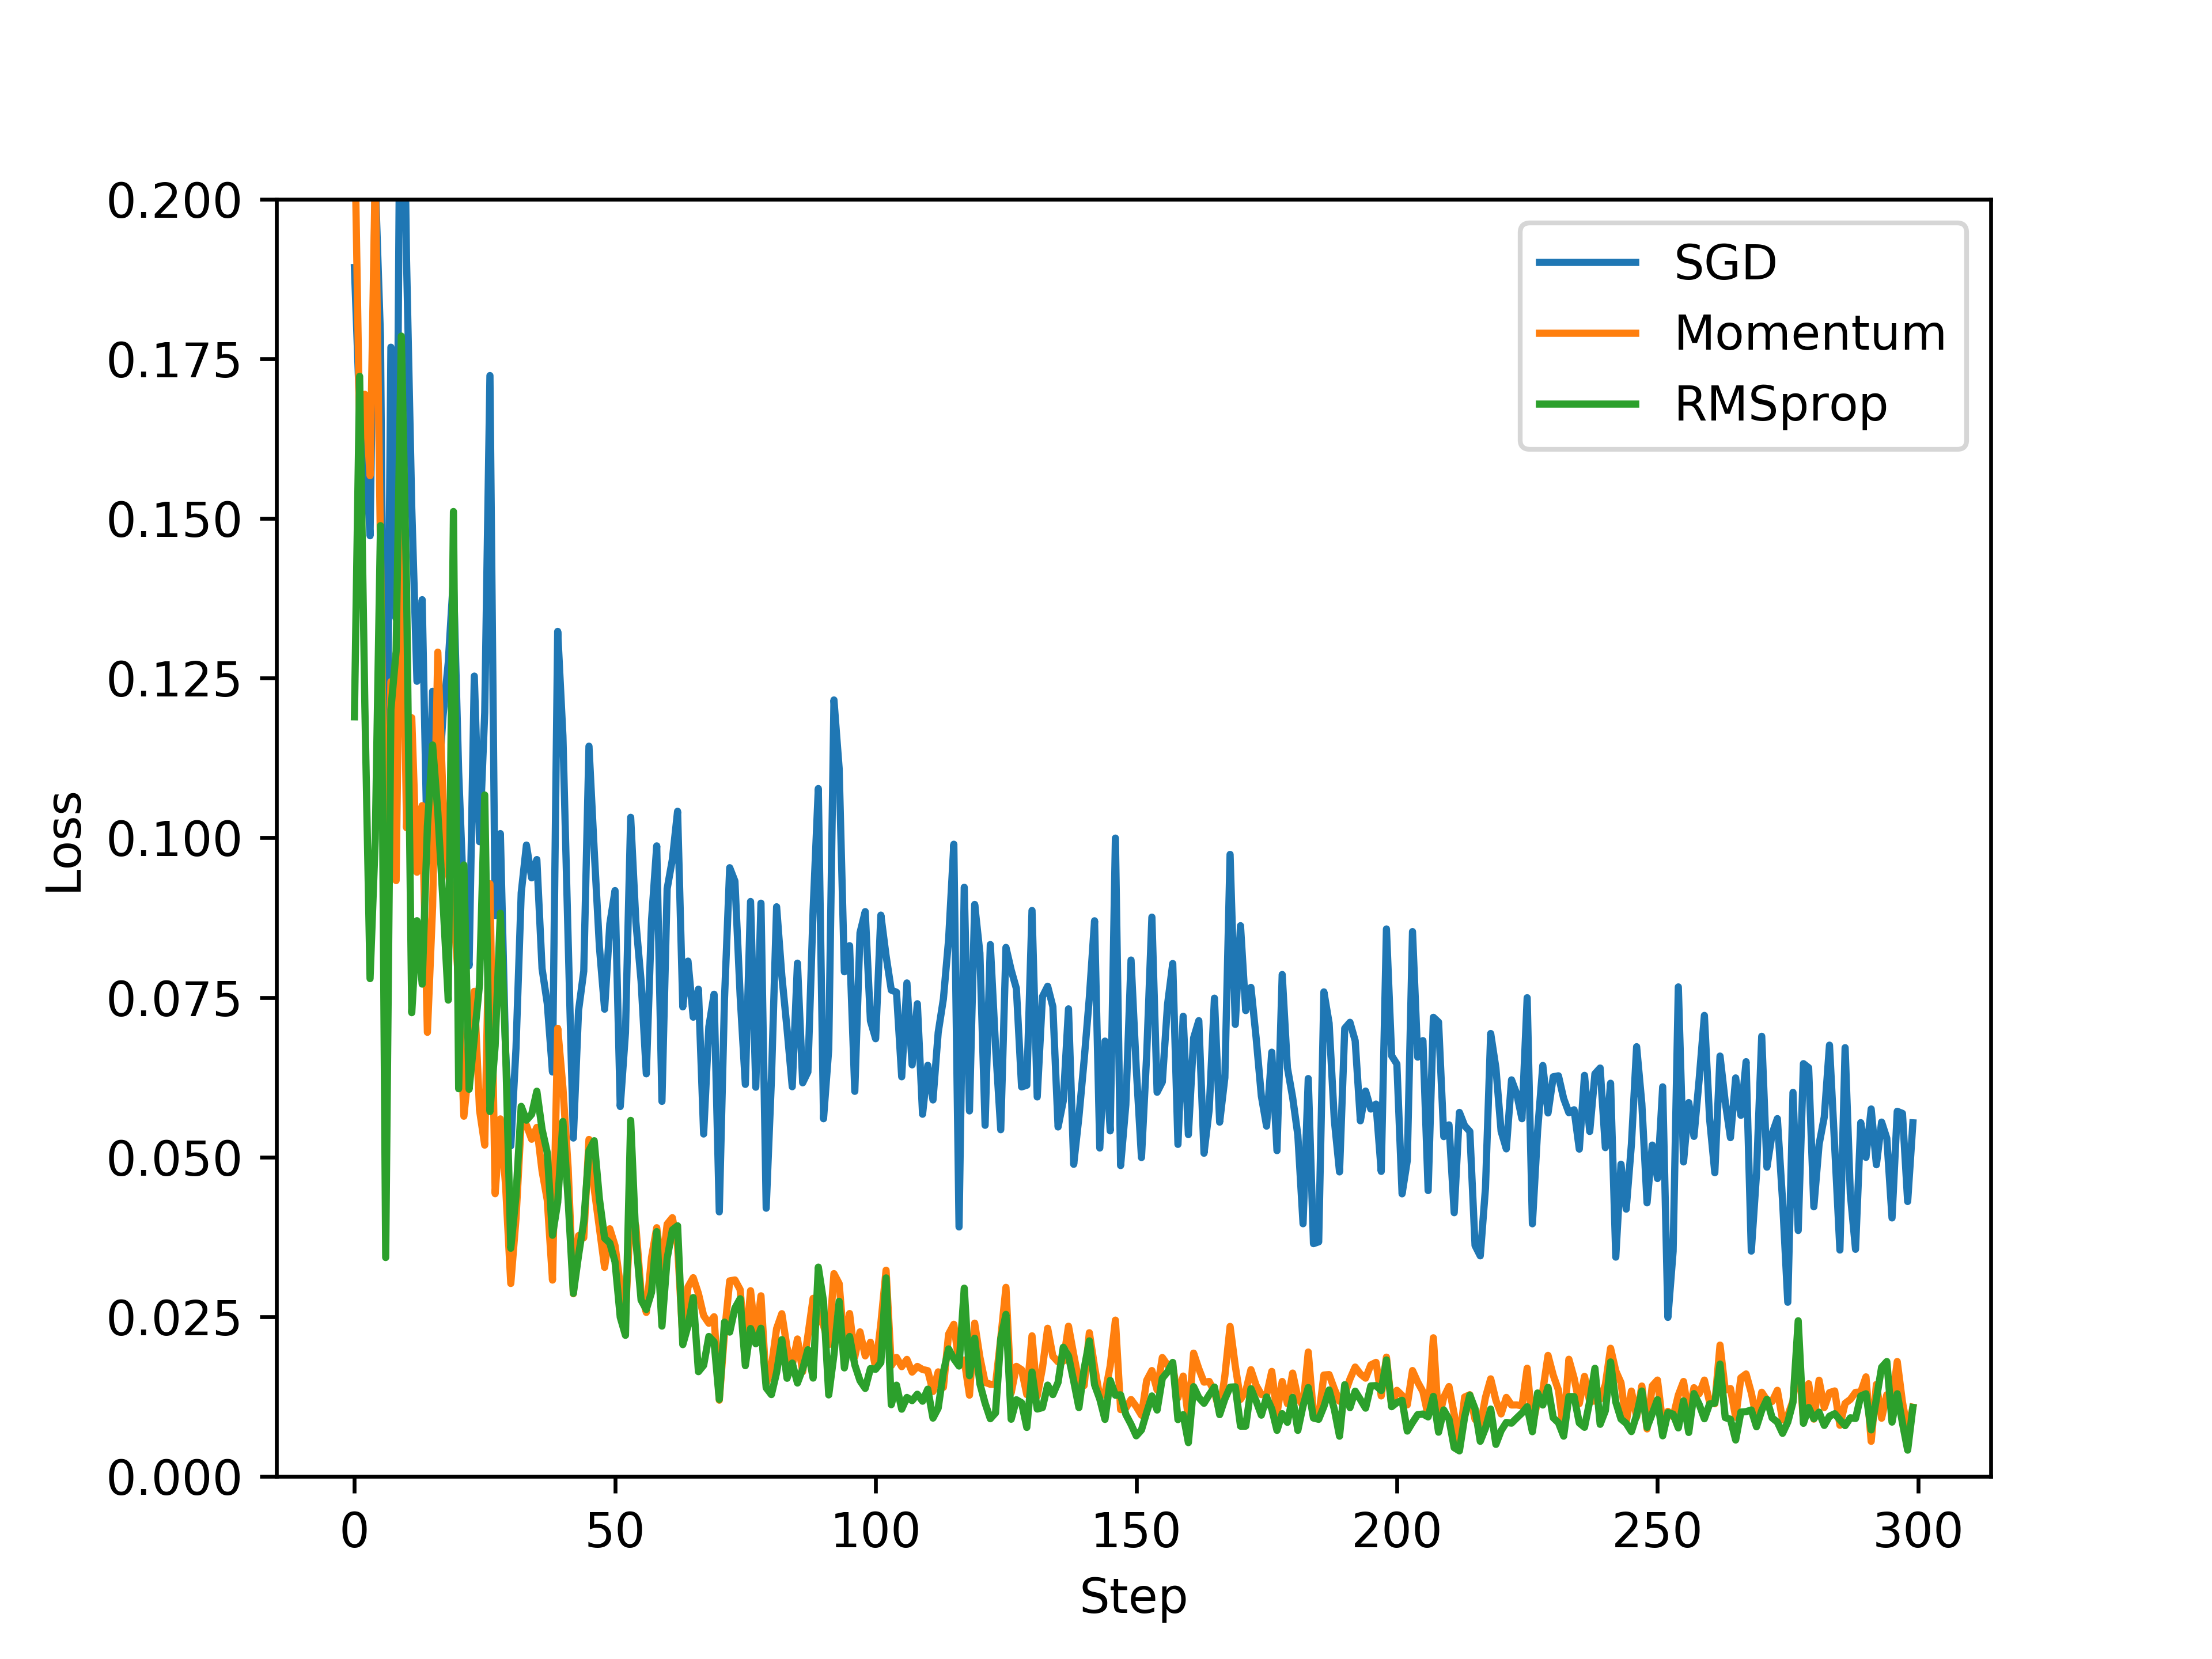
\includegraphics[scale=0.6]{./pic/chapter1/Opt.png}
\end{figure}
\subsection{构造简单的神经网络拟合数据}
原始数据为$y=x^2$的基础上添加随机噪声。原始数据的散点图如下
\begin{center}
\begin{figure}[H]
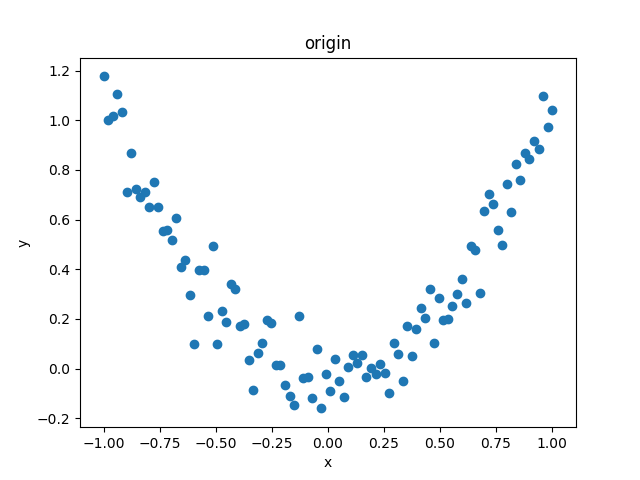
\includegraphics[scale=0.6]{./pic/chapter1/origin.png}
\end{figure}
\end{center}
\begin{python}
#tensorflow 1.2.1
import tensorflow as tf
import matplotlib.pyplot as plt
import numpy as np
tf.set_random_seed(0)
np.random.seed(0)
#生成数据
step = 100
x = np.linspace(-1,1,step).reshape(-1,1)
noise = np.random.normal(0,0.1,size=x.shape)
y = np.power(x,2)+noise

tf_x = tf.placeholder(tf.float32,x.shape)
tf_y = tf.placeholder(tf.float32,x.shape)
l1 =  tf.layers.dense(tf_x,10,tf.nn.relu)
output = tf.layers.dense(l1,1)

loss = tf.losses.mean_squared_error(tf_y,output)
optimizer = tf.train.GradientDescentOptimizer(learning_rate=0.5)
train_op = optimizer.minimize(loss)

sess = tf.Session()
sess.run(tf.global_variables_initializer())
plt.ion()
for step in range(100):
    _,l,pred = sess.run([train_op,loss,output],{tf_x:x,tf_y:y})
    if step%5==0:
        plt.cla()
        plt.scatter(x,y)
        plt.title(r'$y=x^2+noise$')
        plt.plot(x,pred,'r-',lw=2)
        plt.text(0,0.8,'Loss=%.4f'%l,fontdict={'size':10,'color':'blue'})
        plt.xlabel("x")
        plt.ylabel(r"$y=x^2$")
        plt.pause(0.1)
plt.ioff()
plt.show()
\end{python}
最终拟合数据:
\begin{figure}[H]
\includegraphics[scale=0.4]{./pic/chapter1/final.png}
\end{figure}
\section{TensorBoard}
\begin{python}
import tensorflow as tf
import matplotlib.pyplot as plt

tf.set_random_seed(1)
x0 = tf.random_normal((100,2),2,2,tf.float32,0)
y0 = tf.zeros(100)
x1 = tf.random_normal((100,2),-2,2,tf.float32,0)
y1 = tf.ones(100)
x = tf.reshape(tf.stack((x0,x1),axis=1),(200,2))
y = tf.reshape(tf.stack((y0,y1),axis=1),(200,1))
with tf.Session() as sess:
    x = sess.run(x)
    y = sess.run(y)

tf_x = tf.placeholder(tf.float32, x.shape)     # input x
tf_y = tf.placeholder(tf.int32, y.shape)     # input y

# neural network layers
l1 = tf.layers.dense(tf_x, 10, tf.nn.relu)          # hidden layer
output = tf.layers.dense(l1, 2)                     # output layer

loss = tf.losses.sparse_softmax_cross_entropy(labels=tf_y, logits=output)           # compute cost
accuracy = tf.metrics.accuracy(          # return (acc, update_op), and create 2 local variables
            labels=tf.squeeze(tf_y), predictions=tf.argmax(output, axis=1),)[1]
optimizer = tf.train.GradientDescentOptimizer(learning_rate=0.05)
train_op = optimizer.minimize(loss)

sess = tf.Session()                                                                 # control training and others
init_op = tf.group(tf.global_variables_initializer(), tf.local_variables_initializer())
sess.run(init_op)     # initialize var in graph

plt.ion()   # something about plotting
for step in range(100):
    _, acc, pred = sess.run([train_op, accuracy, output], {tf_x: x, tf_y: y})
    if step % 2 == 0:
        plt.cla()
        plt.scatter(x[:, 0], x[:, 1], c=pred.argmax(1), s=100, lw=0, cmap='RdYlGn')
        plt.text(1.5, -4, 'Accuracy=%.2f' % acc, fontdict={'size': 20, 'color': 'red'})
        plt.pause(0.1)
plt.ioff()
plt.show()
\end{python}
\begin{figure}[H]
	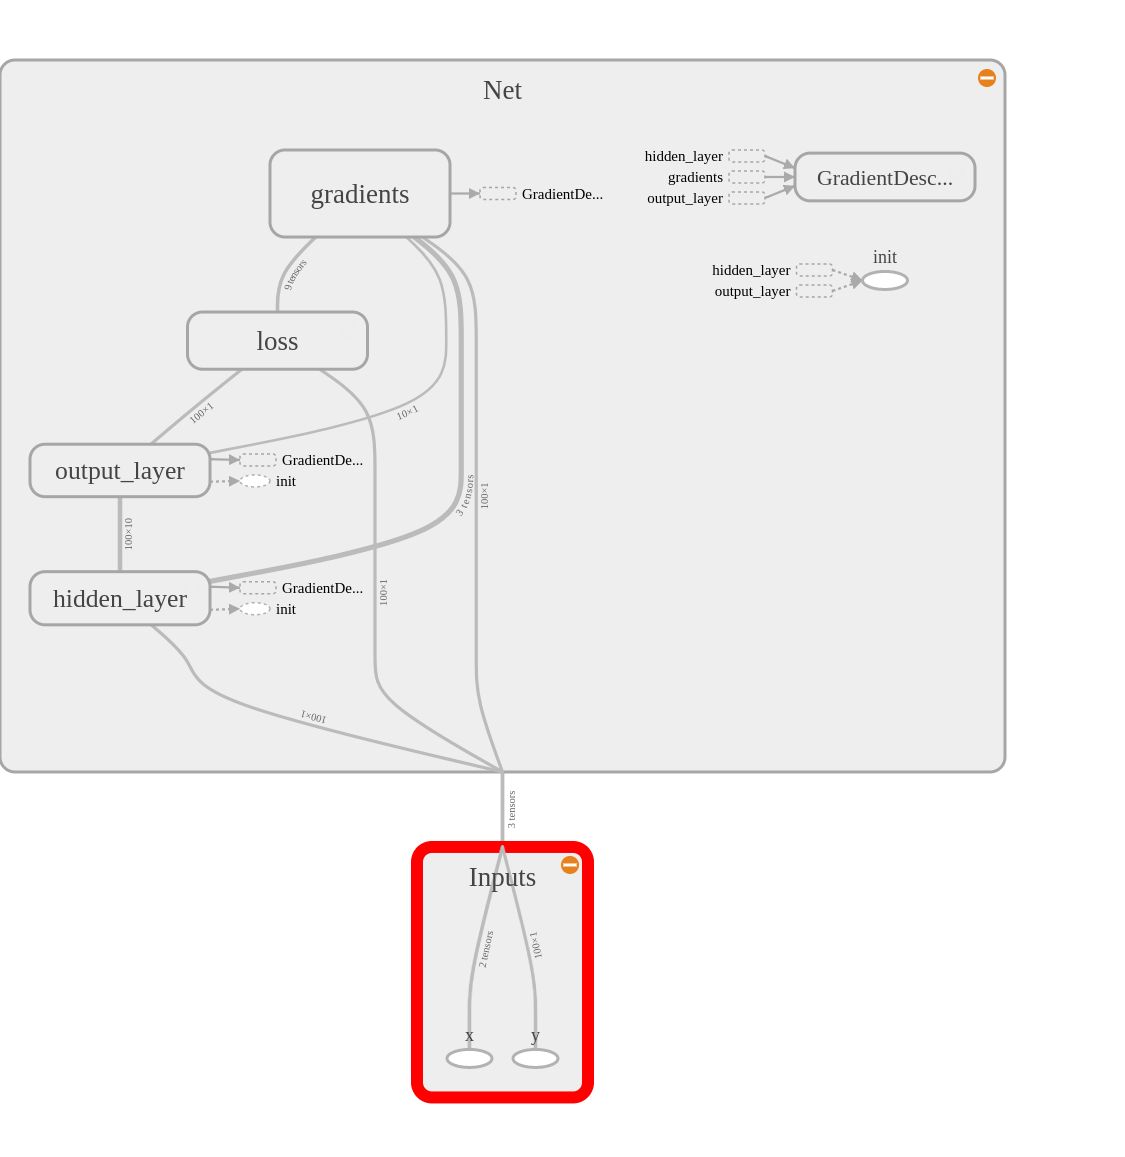
\includegraphics[scale=0.4]{./pic/chapter1/tenbor1.png}
\end{figure}
\subsection{TensorBoard Histogram Dashboard}
TensorBoard Histogram Dashboard 显示TensorFlow图中的Tensor如何随着时间变化。
\subsection{一个简单的例子}
正态分布变量,均值随着和时间移动。TensorFlow有一个操作tf.random\_normal可以完美的达到这个目的。正如通常情况下TensorBoard,我们将用summary op融合数据据。
在这种情况下'tf.summary.histogram'。
这里有一个代码段将生成一些包含正态分布直方图数据的总结,这里均值随着时间增大。
\begin{python}
import tensorflow as tf
k = tf.placeholder(tf.float32)
mean_moving_normal = tf.random_normal(shape=[1000], mean=(5*k), stddev=1)
summaries = tf.summary.histogram('normal/moving_mean',mean_moving_normal)
sess = tf.Session()
writer = tf.summary.FileWriter('./histogram_example')
N = 400
for step in range(N):
    k_val = step/float(N)
    summ = sess.run(summaries,feed_dict={k:k_val})
    writer.add_summary(summ,global_step=step)
\end{python}
在当前代码中运行下边的代码启动TensorFlow载入数据
\begin{python}
tensorboard --logdir=./histogram_example
\end{python}
\begin{center}
\begin{figure}[H]
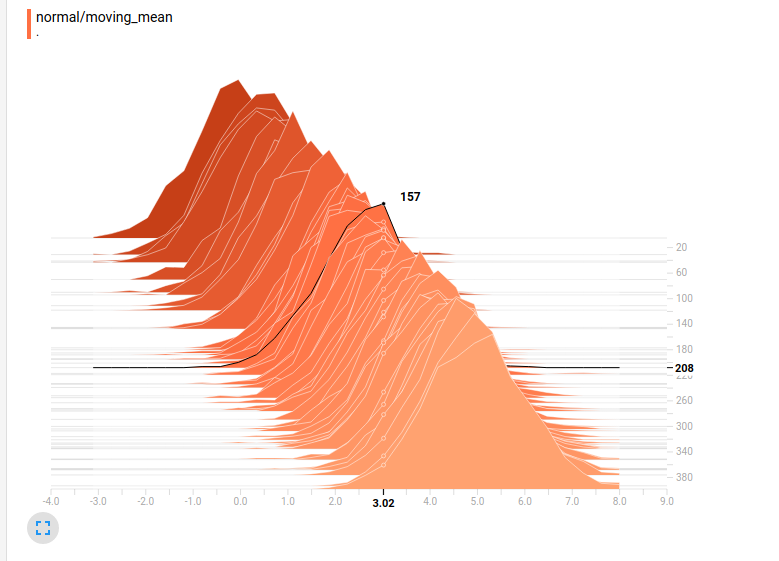
\includegraphics[scale=0.5]{tb_hist1.png}
\end{figure}
\end{center}
tf.summary.histogram接受任一尺寸和大小的Tensor,压缩他们进入直方数据结构组成一些小的数据宽度和数量组层的bin将诶够,例如我们像组成数[0.5,1.1,1.3,2.2,2.9,2.99]成3个bin,我们可以创建三个bin:一个包含0到1之间的一切(0.5),一个包含1-2(1.1,1.3)之间,一个包含2-3(2.2,2.9,2.99)

  TensorFlow用类是的方法创建bins,但是不想我们上面的例子,它不创建整数读额bins,瑞与大型数据,稀疏数据,这样的也许导致上千个bin,bins时指数分布时,一些bins相比于一些非常大数的bin接近于0。然而,可视化指数分布bin时一个技巧,如果高被编码为数量,bin宽度更大的空间,甚至他们有相同的元素,相比较之下统计数量使得豪赌比较变得可能,直方图采集数据仅均匀的bins,这可能导致不幸的人工操作。

在直方图可视化器的每一个切片显示为一个单个的直方图。切片安装步数组织。例老的切片(e.g. step 0)比较靠后变为更深,然而新的slices接近于前景色,颜色更轻,右边的y轴显示了步数。

你可以在直方图上滑动鼠标看到更多的详细星系。你如下面的图你可以看到直方图的时间不为177有一个bin中心在3.78有bin中有34.5个元素。
\begin{center}
\begin{figure}[H]
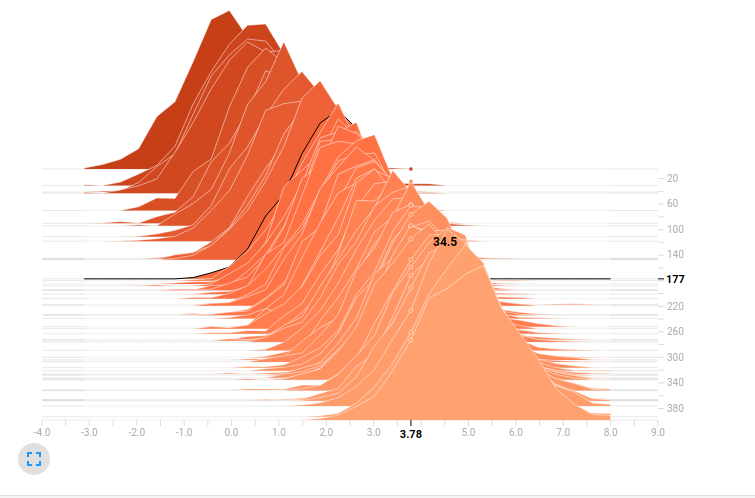
\includegraphics[scale=0.5]{tb_hist2.png}
\end{figure}
\end{center}
你也许注意到注意到直方切片在统计步数和时间上不总是偶数,这是因为TensorBoard用\href{https://en.wikipedia.org/wiki/Reservoir\_sampling}{reservoir sampling}保持直方图的子集,为了节约内存,Reservior sampling保证每个采样有一个相等的可能性被包含进去,但是因为它时一个随机算法,采样并不在每个偶数步发生。
\subsection{Overlay Mode}
控制面板上允许你打开直方图模式为offset为overlay。
在offset模式下,可视化转动45度,因此单个的直方图切片不再展开,而是所有的图华仔一个相同的y轴上。
\begin{center}
\begin{figure}[H]
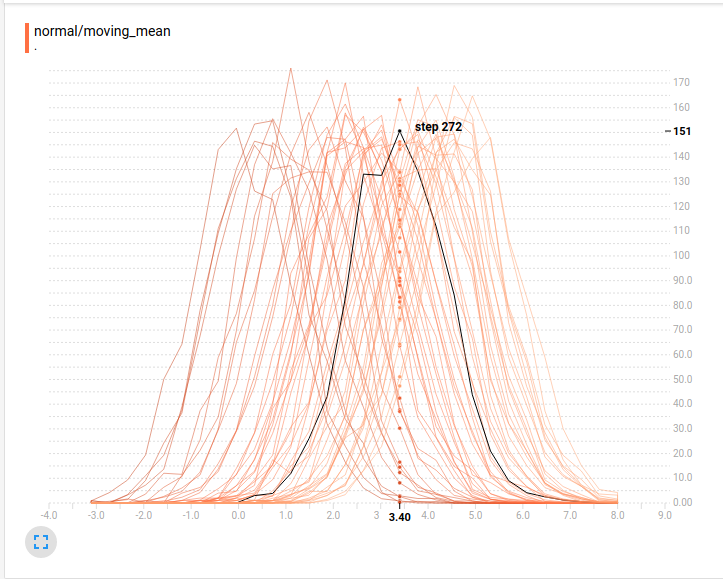
\includegraphics[scale=0.5]{tb_hist3.png}
\end{figure}
\end{center}
现在表上的每个切片被线分开,y轴显示每个bucket项目数量,深色线时老的,早期的时间不,浅色线时最近的新的时间不,你可以用鼠标在表上查看更多的信息。
\begin{center}
\begin{figure}[H]
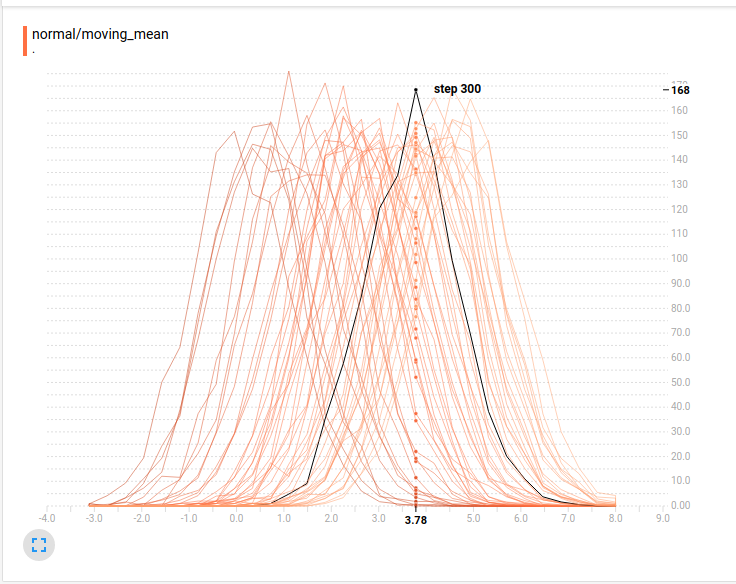
\includegraphics[scale=0.5]{tb_hist4.png}
\end{figure}
\end{center}

overlay可视化在你想直接比较不同直方图的数量。
\subsection{多个分布}
直方图控制面板对多分布下的可视化很有用,当我们通过链接两个不同的正态分布构造一个简单的二两分布,代码如下:
\begin{python}
import tensorflow as tf
k = tf.placeholder(tf.float32)
mean_moving_normal = tf.random_normal(shape=[1000],mean=(3*5),stddev=1)
tf.summary.histogram('normal/moving_mean',mean_moving_normal)
variance_shrinking_normal = tf.random_normal(shape=[100],mean=0,stddev=1-(k))
tf.summary.histogram('normal/shrinking_varance',variance_shrinking_normal)
normal_combined = tf.concat([mean_moving_normal,variance_shrinking_normal],0)
tf.summary.histogram('normal/bimodal',normal_combined)
summaris = tf.summary.merge_all()
sess = tf.Session()
writer = tf.summary.FileWriter('./histgram_example1')
N = 400
for step in range(N):
    k_val = step/float(N)
    summ = sess.run(summaris,feed_dict={k:k_val})
    writer.add_summary(summ,global_step=step)
\end{python}
上面的例子是滑动平均,现在我们已有一个收缩的变量分布。
\begin{center}
\begin{figure}[H]
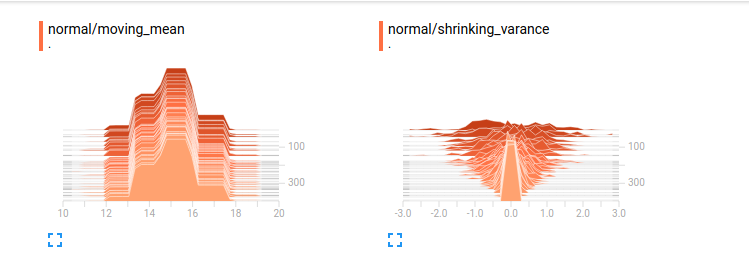
\includegraphics[scale=0.6]{tb_hist5.png}
\end{figure}
\end{center}
当我们链接她们在一起,我们得到一个清晰解释分歧,二进制结构的表格:
\begin{center}
\begin{figure}[H]
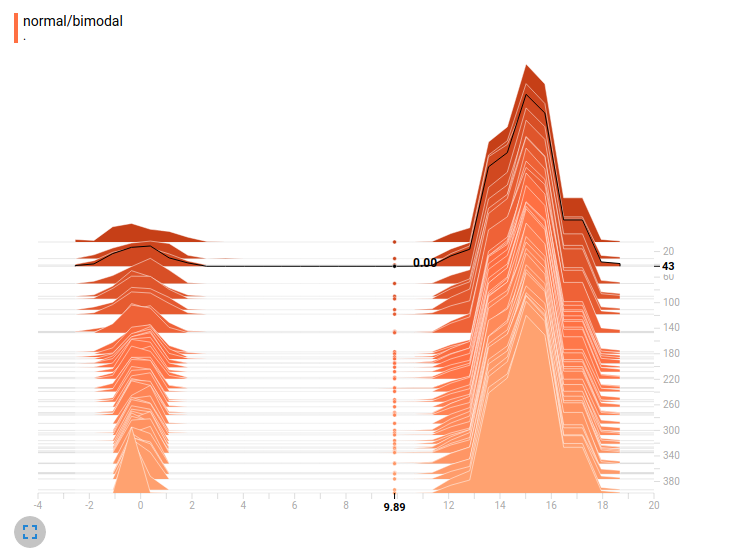
\includegraphics[scale=0.5]{tb_hist6.png}
\end{figure}
\end{center}
\subsection{更多分布}
生成可视化更多分布,结合他们到表中:
\begin{python}
import tensorflow as tf
k = tf.placeholder(tf.float32)
# Make a normal distribution,with a shift mean
mean_moving_normal = tf.random_normal(shape=[1000],mean=(5*k),stddev=1)
tf.summary.histogram('normal/moving_mean',mean_moving_normal)
variance_shrinking_normal = tf.random_normal(shape=[1000],mean=0,stddev=1-(k))
tf.summary.histogram('normal/shinking_variance',variance_shrinking_normal)
normal_combined = tf.concat([mean_moving_normal,variance_shrinking_normal],0)
tf.summary.histogram("normal/bimodal",normal_combined)
#add gamma distribution
gamma = tf.random_gamma(shape=[1000],alpha=k)
tf.summary.histogram('gamma',gamma)
poisson = tf.random_poisson(shape=[1000],lam=k)
tf.summary.histogram('poisson',poisson)
#add a uniform distribution
uniform = tf.random_uniform(shape=[1000],maxval=k*10)
tf.summary.histogram('uniform',uniform)
#finnally combine everything together

all_distributions = [mean_moving_normal,variance_shrinking_normal,gamma,poisson,uniform]
all_combined = tf.concat(all_distributions,0)
tf.summary.histogram('all_combined',all_combined)
summaries = tf.summary.merge_all()
sess = tf.Session()
writer = tf.summary.FileWriter('./histogram_example2')
N = 400
for step in range(N):
    k_val = step/float(N)
    summ = sess.run(summaries,feed_dict={k:k_val})
    writer.add_summary(summ,global_step=step)
\end{python}
\begin{center}
\begin{figure}[H]
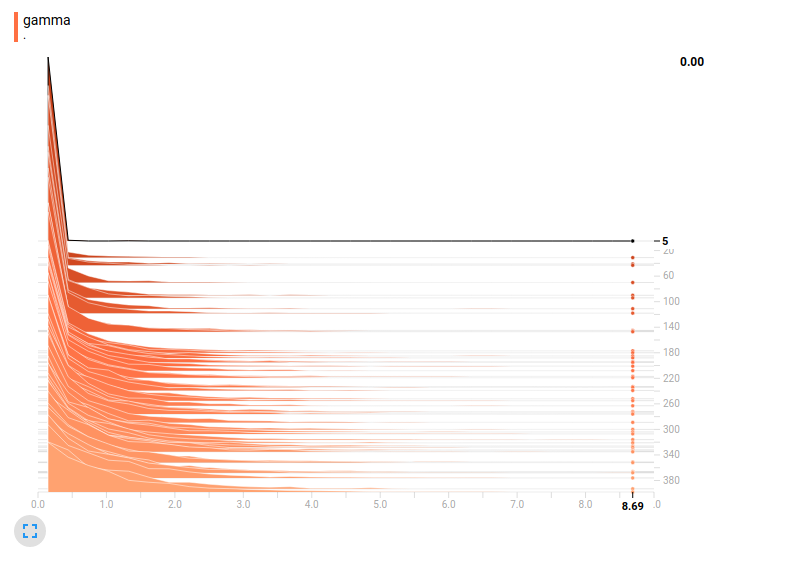
\includegraphics[scale=0.5]{tb_hist7.png}
\end{figure}
\end{center}
\begin{center}
\begin{figure}
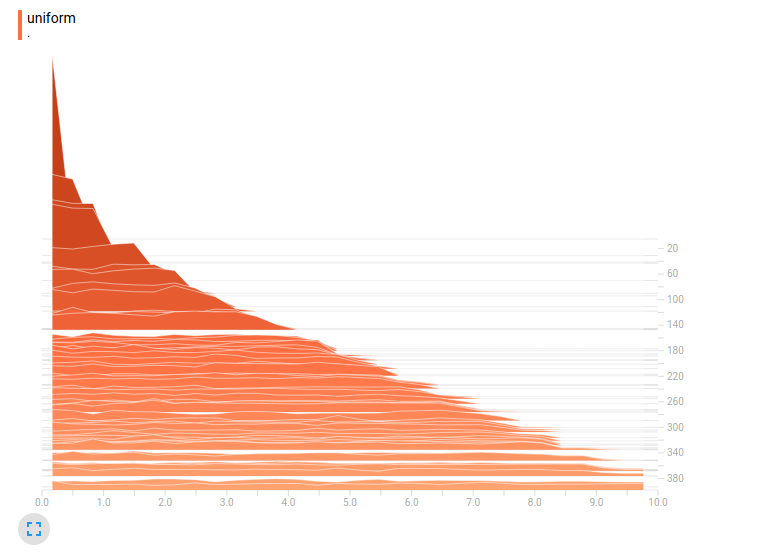
\includegraphics[scale=0.5]{tb_hist9.png}
\end{figure}
\end{center}
\subsection{poisson分布}
\begin{center}
\begin{figure}[H]
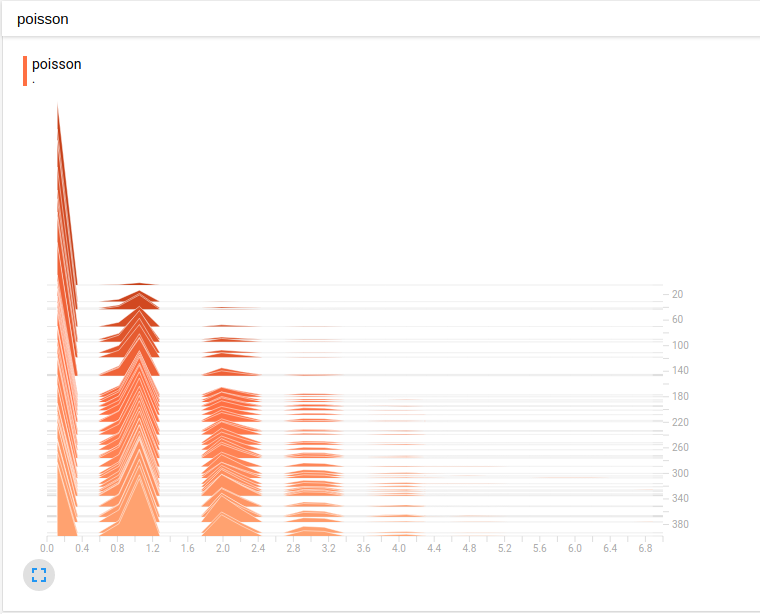
\includegraphics[scale=0.5]{tb_hist10.png}
\end{figure}
\end{center}
poisson分布定义在整数上,因此所有被生成的值都是整数,直方图压缩移动数据到浮点bins,导致可视化在整数值上显示一点点突起。
\subsection{结合所有的数据到一张图向上}
\begin{center}
\begin{figure}[H]
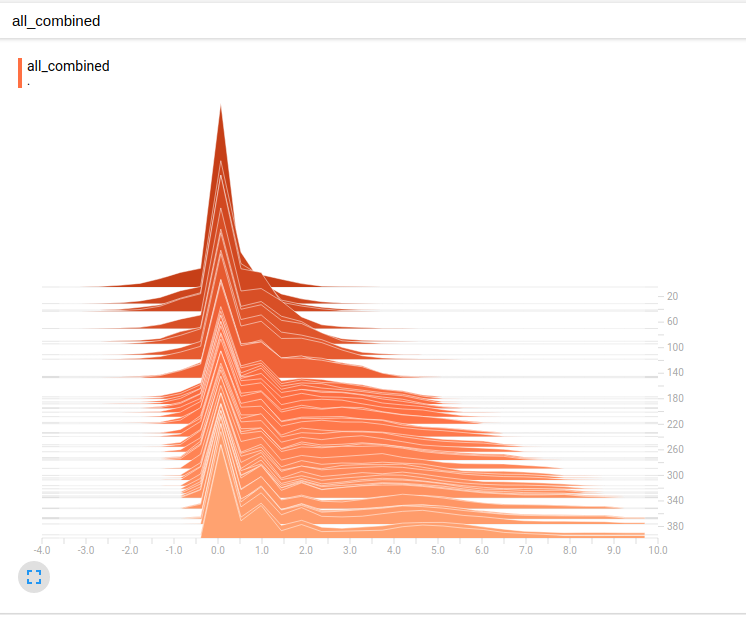
\includegraphics[scale=0.5]{tb_hist11.png}
\end{figure}
\end{center}


\begin{python}
import tensorflow as tf
import matplotlib.pyplot as plt
import numpy as np
tf.set_random_seed(0)
np.random.seed(0)
x = np.linspace(-1,1,100).reshape(-1,1)
noise = np.random.normal(0,0.1,size=x.shape)
y = np.power(x,2)+noise
def gendata():
    t = np.linspace(-1,1,100).reshape(-1,1)
def save():
    print('This is save')
    tf_x = tf.placeholder(tf.float32,x.shape)
    tf_y = tf.placeholder(tf.float32,y.shape)
    l = tf.layers.dense(tf_x,10,tf.nn.relu)
    o = tf.layers.dense(l,1)
    loss = tf.losses.mean_squared_error(tf_y,o)
    train_op = tf.train.GradientDescentOptimizer(learning_rate=0.5).minimize(loss)
    sess = tf.Session()
    sess.run(tf.global_variables_initializer())
    saver = tf.train.Saver()
    for step in range(100):
        sess.run(train_op,{tf_x:x,tf_y:y})
    saver.save(sess,'params',write_meta_graph=False)
    pred,l = sess.run([o,loss],{tf_x:x,tf_y:y})
    plt.figure(1,figsize=(10,5))
    plt.subplot(121)
    plt.scatter(x,y)
    plt.plot(x,pred,'r-',lw=5)
    plt.text(-1,1.2,'save loss=%.4f'%l,fontdict={'size':15,'color':'red'})
def reload():
    print('This is reload')
    tf_x = tf.placeholder(tf.float32,x.shape)
    tf_y = tf.placeholder(tf.float32,y.shape)
    l_ = tf.layers.dense(tf_x,10,tf.nn.relu)
    o_ = tf.layers.dense(l_,1)
    loss_ = tf.losses.mean_squared_error(tf_y,o_)
    sess = tf.Session()
    saver = tf.train.Saver()
    saver.restore(sess,'params')
    pred,l = sess.run([o_,loss_],{tf_x:x,tf_y:y})
    plt.subplot(122)
    plt.scatter(x,y)
    plt.plot(x,pred,'r-',lw=5)
    plt.text(-1,1.2,'Reload Loss=%.4f'%l,fontdict={'size':15,'color':'red'})
    plt.show()
save()
tf.reset_default_graph()
reload()
\end{python}
\section{CNN手写体数据识别}
\subsection{mnist数据集}
手写体数据训练集有55000张手写体数据图片。测试集有10000张图片。每张图片是大小为32*32的灰度图片。
卷积神经网络结构:
\begin{itemize}
	\item 第一层卷积层:卷积核16个,卷积核大小为$5\times5$,strides=1,padding为SAME,激活函数为relu(输出大小为$28\times28\times16$)。
	\item 第一层池化层:池化层大小为2,strides为2($14\times14\times16$)。
第二层卷积层:卷积核32,大小为$5\times5$,strides=1,padding为SAME,激活函数为relu。($14\times14\times32$)
	\item 第二层池化层:池化层大小为2,strides为2($7\times7\times32$)。
	\item flatten:1568。
\end{itemize}
\begin{figure}[H]
	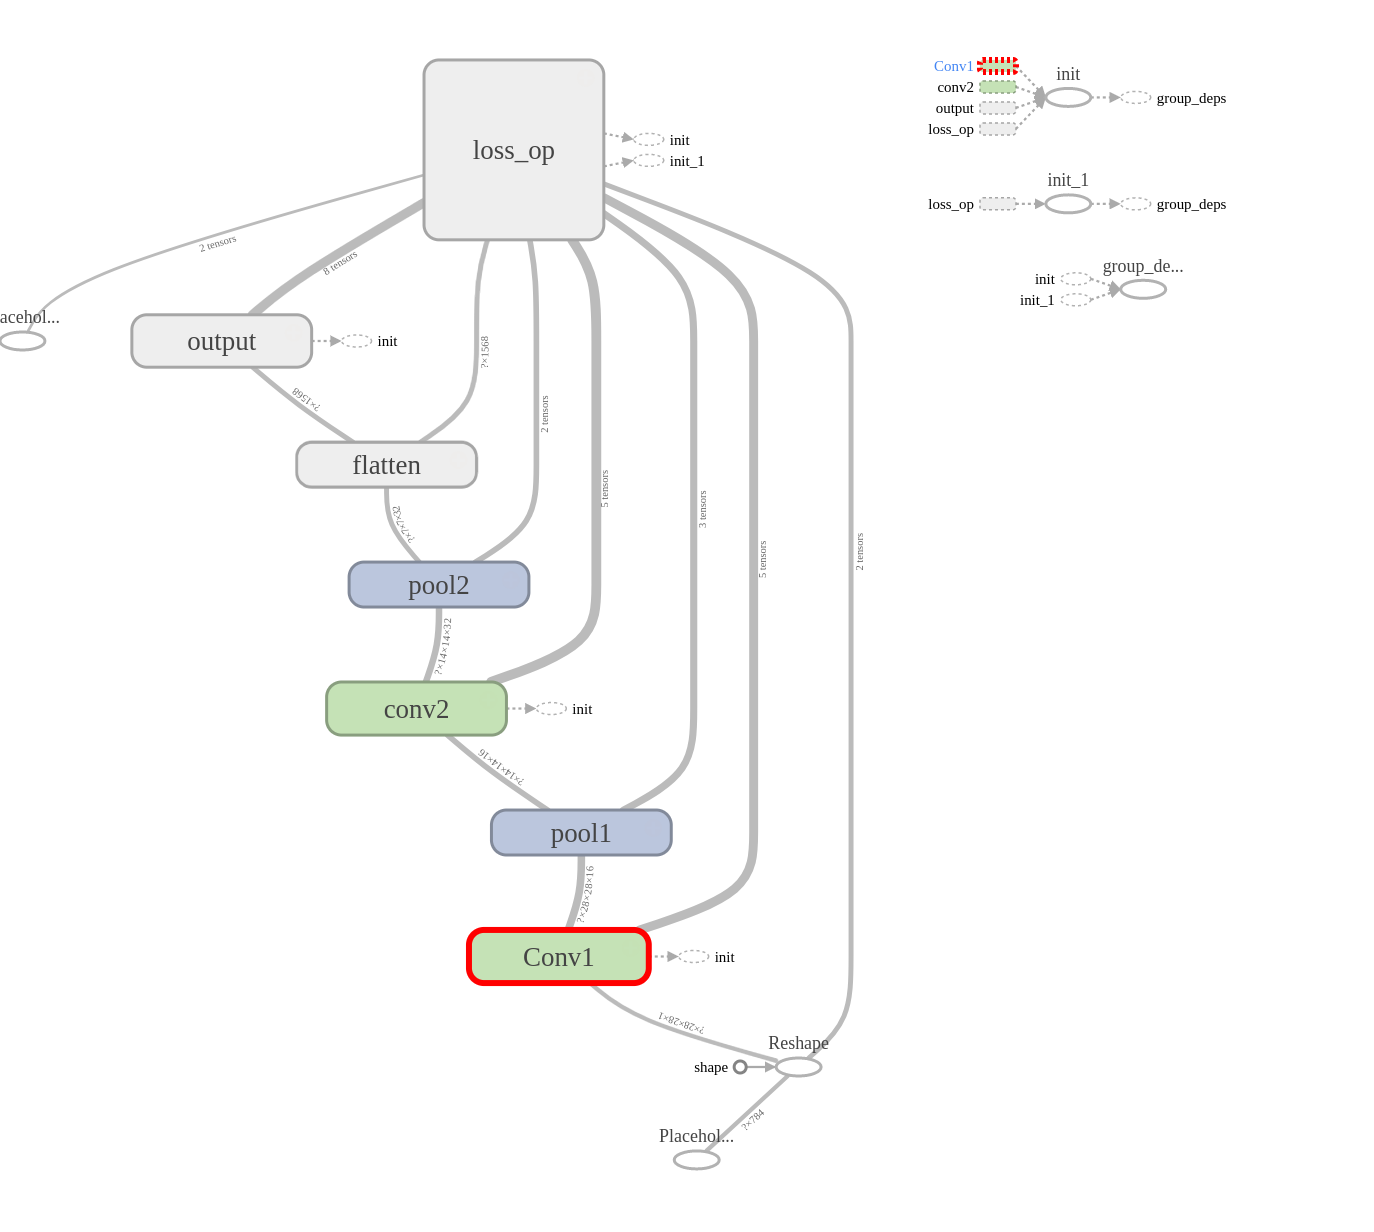
\includegraphics[scale=0.4]{./pic/chapter1/mnist_cnn.png}
\end{figure}
\begin{python}
import tensorflow as tf
import matplotlib.pyplot as plt
import numpy as np
from tensorflow.examples.tutorials.mnist import input_data

tf.set_random_seed(0)
np.random.seed(0)

BATCH_SIZE = 50
LR = 0.001
mnist = input_data.read_data_sets('/home/hpc/文档/mnist_tutorial/mnist',one_hot = True)
test_x = mnist.test.images[:2000]
test_y = mnist.test.labels[:2000]

tf_x = tf.placeholder(tf.float32,[None,28*28])
images = tf.reshape(tf_x,[-1,28,28,1])
tf_y = tf.placeholder(tf.int32,[None,10])
with tf.variable_scope('Conv1'):
    conv1 = tf.layers.conv2d(
            inputs = images,
            filters = 16,
            kernel_size = 5,
            strides = 1,
            padding = 'same',
            activation = tf.nn.relu
        )
    tf.summary.histogram('conv1',conv1)
with tf.variable_scope('pool1'):
    pool1 = tf.layers.max_pooling2d(
            conv1,
            pool_size=2,
            strides =2
        )
    tf.summary.histogram('max_pool1',pool1)
with tf.variable_scope('conv2'):
    conv2 = tf.layers.conv2d(pool1,32,5,1,'SAME',activation=tf.nn.relu)
    tf.summary.histogram('conv2',conv2)
with tf.variable_scope('pool2'):
    pool2 = tf.layers.max_pooling2d(conv2,2,2)
    tf.summary.histogram('max_pool',pool2)
with tf.variable_scope('flatten'):
    flat = tf.reshape(pool2,[-1,7*7*32])
with tf.variable_scope('output'):
    output = tf.layers.dense(flat,10)
with tf.variable_scope('loss_op'):
    loss = tf.losses.softmax_cross_entropy(onehot_labels=tf_y,logits=output)
    train_op = tf.train.AdamOptimizer(LR).minimize(loss)
    accuracy = tf.metrics.accuracy(labels = tf.argmax(tf_y,axis=1),predictions=tf.argmax(output,axis=1),)[1]
    tf.summary.scalar('loss',loss)
    tf.summary.scalar('accuracy',accuracy)
sess = tf.Session()
merge_op = tf.summary.merge_all()
init_op = tf.group(tf.global_variables_initializer(),tf.local_variables_initializer())
sess.run(init_op)
writer = tf.summary.FileWriter('./log',sess.graph)
for step in range(600):
    b_x,b_y = mnist.train.next_batch(BATCH_SIZE)
    _,loss_,result = sess.run([train_op,loss,merge_op],{tf_x:b_x,tf_y:b_y})
    writer.add_summary(result,step)
    if step%50 == 0:
        accuracy_,flat_representation = sess.run([accuracy,flat],{tf_x:test_x,tf_y:test_y})
        print('Step:',step,'| train loss:%.4f'%loss_,'|test accuracy:%.2f'%accuracy_)
test_output = sess.run(output,{tf_x:test_x[:10]})
pred_y = np.argmax(test_output,1)
\end{python}
\section{RNN}
\subsection{向量字表示}
\subsubsection{Vector Representation of Words}
通常图像或音频系统处理的是由图片中所有单个原始像素点强度值或者音频中功率谱密度的强度值,把它们编码成丰富、高维度的向量数据集。对于物体或语音识别这一类的任务,我们所需的全部信息已经都存储在原始数据中(显然人类本身就是依赖原始数据进行日常的物体或语音识别的)。然后,自然语言处理系统通常将词汇作为离散的单一符号,例如 "cat" 一词或可表示为 Id537 ,而 "dog" 一词或可表示为 Id143。这些符号编码毫无规律,无法提供不同词汇之间可能存在的关联信息。换句话说,在处理关于 "dogs" 一词的信息时,模型将无法利用已知的关于 "cats" 的信息(例如,它们都是动物,有四条腿,可作为宠物等等)。可见,将词汇表达为上述的独立离散符号将进一步导致数据稀疏,使我们在训练统计模型时不得不寻求更多的数据。而词汇的向量表示将克服上述的难题。向量空间模型 (VSMs)将词汇表达(嵌套)于一个连续的向量空间中,语义近似的词汇被映射为相邻的数据点。向量空间模型在自然语言处理领域中有着漫长且丰富的历史,不过几乎所有利用这一模型的方法都依赖于 分布式假设,其核心思想为出现于上下文情景中的词汇都有相类似的语义。采用这一假设的研究方法大致分为以下两类:基于计数的方法 (e.g. 潜在语义分析), 和 预测方法 (e.g. 神经概率化语言模型).

其中它们的区别在如下论文中又详细阐述 \href{http://clic.cimec.unitn.it/marco/publications/acl2014/baroni-etal-countpredict-acl2014.pdf}{Baroni :et al},不过简而言之:基于计数的方法计算某词汇与其邻近词汇在一个大型语料库中共同出现的频率及其它统计量,然后将这些统计量映射到一个小型且稠密的向量中。预测方法则试图直接从某词汇的邻近词汇对其进行预测,在此过程中利用已经学习到的小型且稠密的嵌套向量。

Word2vec是一种可以进行高效率词嵌套学习的预测模型。其两种变体分别为:连续词袋模型(CBOW)及Skip-Gram模型。从算法角度看,这两种方法非常相似,其区别为CBOW根据源词上下文词汇('the cat sits on the')来预测目标词汇(例如,‘mat’),而Skip-Gram模型做法相反,它通过目标词汇来预测源词汇。Skip-Gram模型采取CBOW的逆过程的动机在于:CBOW算法对于很多分布式信息进行了平滑处理(例如将一整段上下文信息视为一个单一观察量)。很多情况下,对于小型的数据集,这一处理是有帮助的。相形之下,Skip-Gram模型将每个“上下文-目标词汇”的组合视为一个新观察量,这种做法在大型数据集中会更为有效。本教程余下部分将着重讲解Skip-Gram模型。
\subsubsection{处理噪声的对比训练}
神经概率化语言模型通常使用极大似然法 (ML) 进行训练,其中通过 softmax function 来最大化当提供前一个单词 h (代表 "history"),后一个单词的概率$w_t$(目标词概率)
\begin{equation*}
P(w_t|h)=softmax(score(w_t,h))=\frac{exp\left\{score(w_t,h)\right\}}{\Sigma_{Word w' in Vocab}exp\left\{score(w',h)\right\}}
\end{equation*}
当 $score(w_t,h)$ 计算了文字 $w_t$ 和 上下文 h 的相容性(通常使用向量积)。我们使用对数似然函数来训练训练集的最大值,比如通过:
\begin{equation*}
J_{ML} = logP(w_t|h)=score(w_t,h)-log(\Sigma_{Word w' in Vocab}exp\left\{score(w',h)\right\})
\end{equation*}
这里提出了一个解决语言概率模型的合适的通用方法。然而这个方法实际执行起来开销非常大,因为我们需要去计算并正则化当前上下文环境 h 中所有其它 V 单词 w' 的概率得分,在每一步训练迭代中。
\begin{figure}[H]
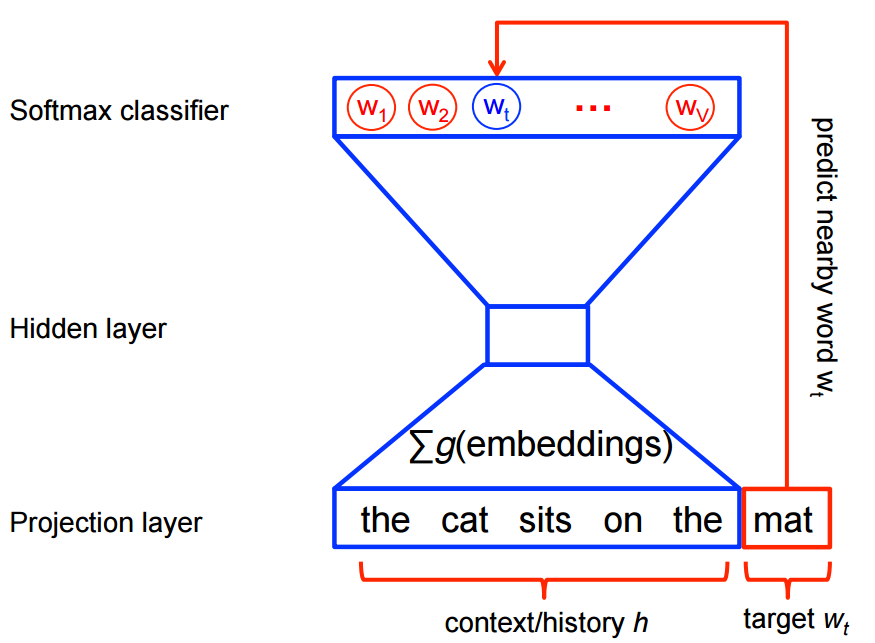
\includegraphics[scale=0.5]{softmax-nplm.png}
\caption{CBOW方法}
\end{figure}
从另一个角度来说,当使用word2vec模型时,我们并不需要对概率模型中的所有特征进行学习。而CBOW模型和Skip-Gram模型为了避免这种情况发生,使用一个二分类器(逻辑回归)在同一个上下文环境里从 k 虚构的 (噪声) 单词$\hat{w}$区分真正的目标单词$w_t$,下面详细参数CBOW模型,对于Skip-Gram模型只要简单的反向操作即可。
\begin{center}
\begin{figure}[H]
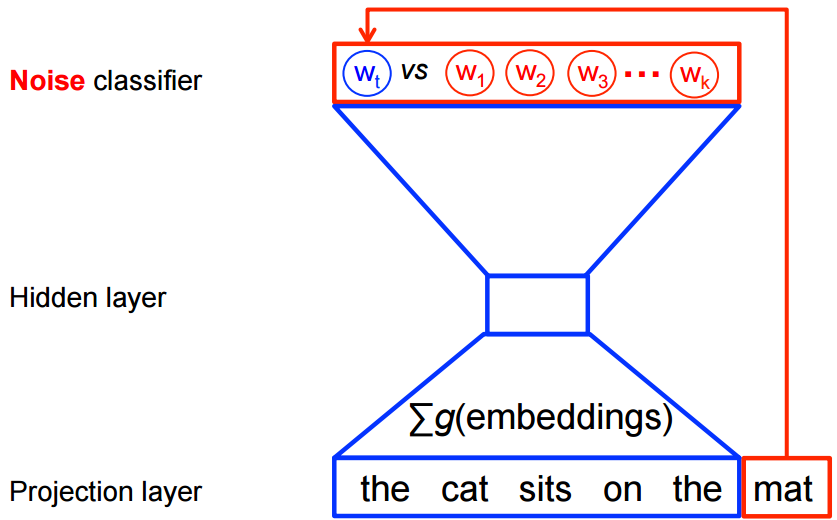
\includegraphics[scale=0.5]{nce-nplm.png}
\caption{Skip-Gram}
\end{figure}
\end{center}
从数学的角度来说,我们的目标是对每个样本最大化:
\begin{equation*}
J_{NEG}=logQ_{\theta}(D=1|w_t,h)+k\underset{\hat{w}\sim P_{noise}}{E}[logQ_{\theta}(D=0|\hat{\omega},h)]
\end{equation*}
其中$Q_{\theta}(D=1|w,h)$代表的是当前上下文h,根据所学得嵌套向量$\theta$目标单词 w 使用二分类逻辑回归计算得出的概率。在实践中,我们通过在噪声分布中绘制比对文字来获得近似的期望值(通过计算\href{https://en.wikipedia.org/wiki/Monte_Carlo_integration}{蒙特卡洛平均值})。

当真实地目标单词被分配到较高的概率,同时噪声单词的概率很低时,目标函数也就达到最大值了。从技术层面来说,这种方法叫做\href{http://papers.nips.cc/paper/5021-distributed-representations-of-words-and-phrases-and-their-compositionality.pdf}{负抽样},而且使用这个损失函数在数学层面上也有很好的解释:这个更新过程也近似于softmax函数的更新。这在计算上将会有很大的优势,因为当计算这个损失函数时,只是有我们挑选出来的 k 个 噪声单词,而没有使用整个语料库 V。这使得训练变得非常快。我们实际上使用了与\href{http://papers.nips.cc/paper/5165-learning-word-embeddings-efficiently-with-noise-contrastive-estimation.pdf}{noise-contrastive estimation (NCE)}介绍的非常相似的方法,这在TensorFlow中已经封装了一个很便捷的函数tf.nn.nce\_loss()。

\subsubsection{Skip-gram模型}
下面来看一下这个数据集

the quick brown fox jumped over the lazy dog

我们首先对一些单词以及它们的上下文环境建立一个数据集。我们可以以任何合理的方式定义‘上下文’,而通常上这个方式是根据文字的句法语境的(使用语法原理的方式处理当前目标单词可以看一下这篇文献 \href{https://levyomer.files.wordpress.com/2014/04/dependency-based-word-embeddings-acl-2014.pdf}{Levy et al.},比如说把目标单词左边的内容当做一个‘上下文’,或者以目标单词右边的内容,等等。现在我们把目标单词的左右单词视作一个上下文, 使用大小为1的窗口,这样就得到这样一个由(上下文, 目标单词) 组成的数据集:

([the, brown], quick), ([quick, fox], brown), ([brown, jumped], fox), ...

前文提到Skip-Gram模型是把目标单词和上下文颠倒过来,所以在这个问题中,举个例子,就是用'quick'来预测 'the' 和 'brown' ,用 'brown' 预测 'quick' 和 'brown' 。因此这个数据集就变成由(输入, 输出)组成的:

(quick, the), (quick, brown), (brown, quick), (brown, fox), ...

目标函数通常是对整个数据集建立的,但是本问题中要对每一个样本(或者是一个batch\_size 很小的样本集,通常设置为16 <= batch\_size <= 512)在同一时间执行特别的操作,称之为\href{https://en.wikipedia.org/wiki/Stochastic_gradient_descent}{随机梯度下降 (SGD)}。我们来看一下训练过程中每一步的执行。

假设用 t 表示上面这个例子中quick 来预测 the 的训练的单个循环。用 num\_noise 定义从噪声分布中挑选出来的噪声(相反的)单词的个数,通常使用一元分布,P(w)。为了简单起见,我们就定num\_noise=1,用 sheep 选作噪声词。接下来就可以计算每一对观察值和噪声值的损失函数了,每一个执行步骤就可表示为:
\begin{equation*}
J_{NEG}^{(t)}=logQ_{\theta}(D=1|the,quick)+log(Q_{\theta}(D=0|sleep,quick))
\end{equation*}
整个计算过程的目标是通过更新嵌套参数$\theta$来逼近目标函数(这个例子中就是使目标函数最大化)。为此我们要计算损失函数中嵌套参数$\theta$的梯度,比如\[\frac{\partial}{\partial}J_{NEG}\]
(幸好TensorFlow封装了工具函数可以简单调用!)。对于整个数据集,当梯度下降的过程中不断地更新参数,对应产生的效果就是不断地移动每个单词的嵌套向量,直到可以把真实单词和噪声单词很好得区分开。

我们可以把学习向量映射到2维中以便我们观察,其中用到的技术可以参考 \href{http://lvdmaaten.github.io/tsne/}{t-SNE 降维技术}。当我们用可视化的方式来观察这些向量,就可以很明显的获取单词之间语义信息的关系,这实际上是非常有用的。当我们第一次发现这样的诱导向量空间中,展示了一些特定的语义关系,这是非常有趣的,比如文字中 male-female,gender 甚至还有 country-capital 的关系, 如下方的图所示 (也可以参考 \href{http://www.aclweb.org/anthology/N13-1090}{Mikolov et al.}, 2013论文中的例子)。
\begin{center}
\begin{figure}[H]
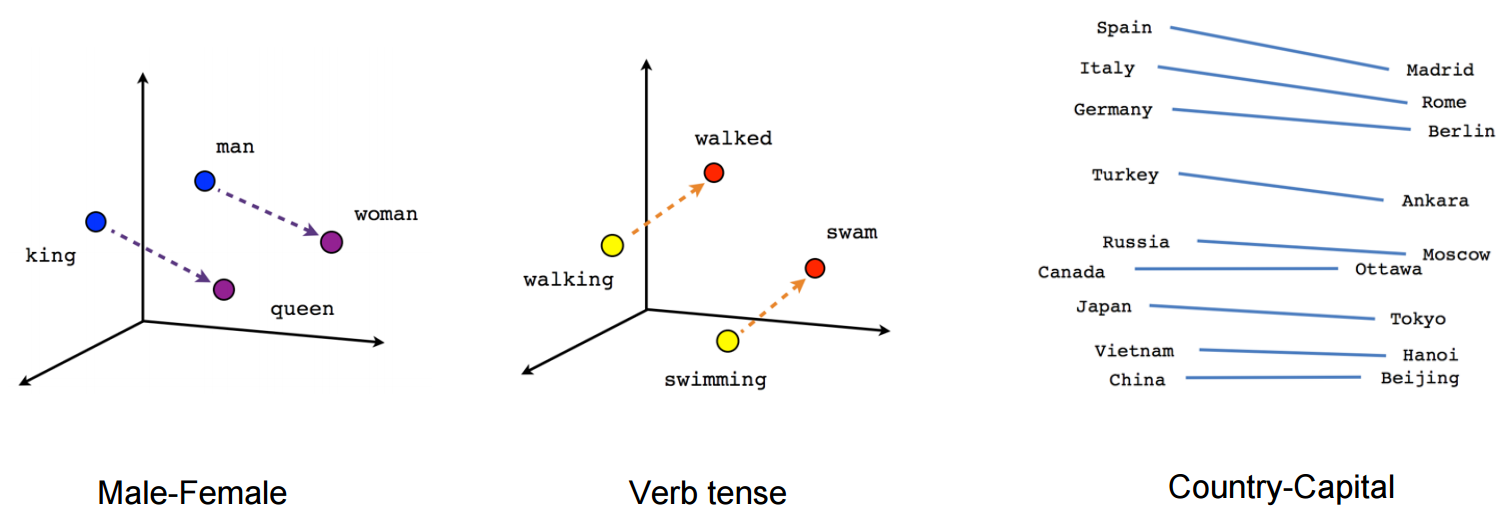
\includegraphics[scale=0.5]{linear-relationships.png}
\end{figure}
\end{center}
这也解释了为什么这些向量在传统的NLP问题中可作为特性使用,比如用在对一个演讲章节打个标签,或者对一个专有名词的识别 (看看如下这个例子 \href{https://arxiv.org/pdf/1103.0398v1.pdf}{Collobert et al.}或者 \href{http://www.aclweb.org/anthology/P10-1040}{Turian et al.})。

不过现在让我们用它们来画漂亮的图表吧!

这里谈得都是嵌套,那么先来定义一个嵌套参数矩阵。我们用唯一的随机值来初始化这个大矩阵。
\begin{python}
embeddings = tf.Variable(
    tf.random_uniform([vocabulary_size, embedding_size], -1.0, 1.0))
\end{python}
对噪声-比对的损失计算就使用一个逻辑回归模型。对此,我们需要对语料库中的每个单词定义一个权重值和偏差值。(也可称之为输出权重 与之对应的 输入嵌套值)。定义如下:
\begin{python}
nce_weights = tf.Variable(
  tf.truncated_normal([vocabulary_size, embedding_size],
                      stddev=1.0 / math.sqrt(embedding_size)))
nce_biases = tf.Variable(tf.zeros([vocabulary_size]))
\end{python}我们有了这些参数之后,就可以定义Skip-Gram模型了。简单起见,假设我们已经把语料库中的文字整型化了,这样每个整型代表一个单词(细节请查看\_basic.py)。Skip-Gram模型有两个输入。一个是一组用整型表示的上下文单词,另一个是目标单词。给这些输入建立占位符节点,之后就可以填入数据了。
\begin{python}
train_inputs = tf.placeholder(tf.int32, shape=[batch_size])
train_labels = tf.placeholder(tf.int32, shape=[batch_size, 1])
\end{python}
然后我们需要对批数据中的单词建立嵌套向量,TensorFlow提供了方便的工具函数。
\begin{python}
embed = tf.nn.embedding_lookup(embeddings, train_inputs)
\end{python}
好了,现在我们有了每个单词的嵌套向量,接下来就是使用噪声-比对的训练方式来预测目标单词。
\begin{python}
loss = tf.reduce_mean(
  tf.nn.nce_loss(nce_weights, nce_biases, embed, train_labels,
                 num_sampled, vocabulary_size))
\end{python}
我们对损失函数建立了图形节点,然后我们需要计算相应梯度和更新参数的节点,比如说在这里我们会使用随机梯度下降法,TensorFlow也已经封装好了该过程。
\begin{python}
optimizer = tf.train.GradientDescentOptimizer(learning_rate=1.0).minimize(loss)
\end{python}
\subsubsection{训练过程}
训练的过程很简单,只要在循环中使用feed\_dict不断给占位符填充数据,同时调用 session.run即可。
\begin{python}
for inputs, labels in generate_batch(...):
  feed_dict = {training_inputs: inputs, training_labels: labels}
  _, cur_loss = session.run([optimizer, loss], feed_dict=feed_dict)
\end{python}
\subsubsection{嵌套学习结果可视化}
\begin{center}
\begin{figure}[H]
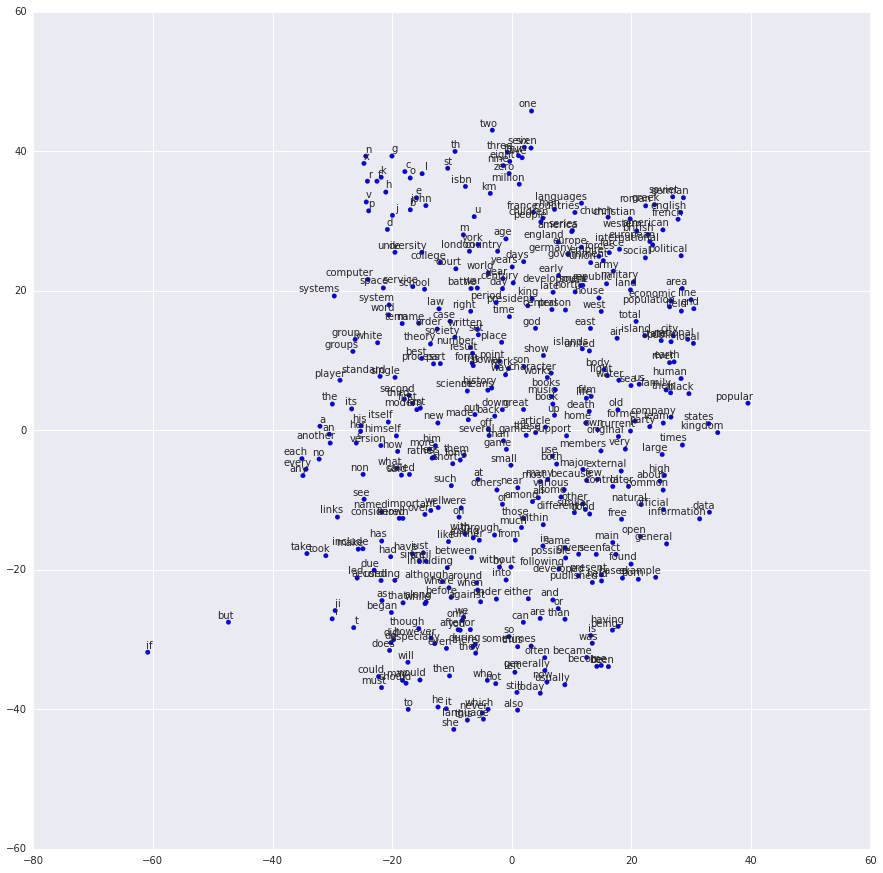
\includegraphics[scale=0.5]{tsne.png}
\end{figure}
\end{center}
Et voila! 与预期的一样,相似的单词被聚类在一起。对word2vec模型更复杂的实现需要用到TensorFlow一些更高级的特性,具体是实现可以参考\href{https://github.com/bleedingfight/models/tree/master/tutorials/embedding}{word2vec.py}\subsubsection{嵌套学习的评估:类比推理}
词嵌套在NLP的预测问题中是非常有用且使用广泛地。如果要检测一个模型是否是可以成熟地区分词性或者区分专有名词的模型,最简单的办法就是直接检验它的预测词性、语义关系的能力,比如让它解决形如king is to queen as father is to ?这样的问题。这种方法叫做类比推理 ,可参考Mikolov and colleagues,数据集下载地址为:\href{https://word2vec.googlecode.com/svn/trunk/questions-words.txt}{questions-words.txt} 。
To see how we do this evaluation如何执行这样的评估,可以看build\_eval\_graph()和 eval()这两个函数在下面源码中的使用 \href{https://github.com/bleedingfight/models/tree/master/tutorials/embedding}{word2vec.py}

超参数的选择对该问题解决的准确性有巨大的影响。想要模型具有很好的表现,需要有一个巨大的训练数据集,同时仔细调整参数的选择并且使用例如二次抽样的一些技巧。不过这些问题已经超出了本教程的范围。
\subsubsection{优化实现}
以上简单的例子展示了TensorFlow的灵活性。比如说,我们可以很轻松得用现成的tf.nn.sampled\_softmax\_loss()来代替tf.nn.nce\_loss()构成目标函数。如果你对损失函数想做新的尝试,你可以用TensorFlow手动编写新的目标函数的表达式,然后用控制器执行计算。这种灵活性的价值体现在,当我们探索一个机器学习模型时,我们可以很快地遍历这些尝试,从中选出最优。

一旦你有了一个满意的模型结构,或许它就可以使实现运行地更高效(在短时间内覆盖更多的数据)。比如说,在本教程中使用的简单代码,实际运行速度都不错,因为我们使用Python来读取和填装数据,而这些在TensorFlow后台只需执行非常少的工作。如果你发现你的模型在输入数据时存在严重的瓶颈,你可以根据自己的实际问题自行实现一个数据阅读器,参考 新的数据格式。对于Skip-Gram 模型,我们已经完成了如下这个例子 \href{https://github.com/bleedingfight/models/tree/master/tutorials/embedding}{word2vec.py}。

如果I/O问题对你的模型已经不再是个问题,并且想进一步地优化性能,或许你可以自行编写TensorFlow操作单元,详见 添加一个新的操作。相应的,我们也提供了Skip-Gram模型的例子 \href{https://github.com/bleedingfight/models/tree/master/tutorials/embedding}{optimized.py}。请自行调节以上几个过程的标准,使模型在每个运行阶段有更好地性能。
\subsection{RNN}
此教程将展示如何在高难度的语言模型中训练循环神经网络。该问题的目标是获得一个能确定语句概率的概率模型。为了做到这一点,通过之前已经给出的词语来预测后面的词语。我们将使用 PTB(Penn Tree Bank) 数据集,这是一种常用来衡量模型的基准,同时它比较小而且训练起来相对快速。

语言模型是很多有趣难题的关键所在,比如语音识别,机器翻译,图像字幕等。它很有意思--可以参看 here。

本教程的目的是重现 \href{http://arxiv.org/abs/1409.2329}{Zaremba et al., 2014} 的成果,他们在 PTB 数据集上得到了很棒的结果。
\subsubsection{下载及准备数据}
本教程需要的数据在 data/ 路径下,来源于 Tomas Mikolov 网站上的\href{http://www.fit.vutbr.cz/~imikolov/rnnlm/simple-examples.tg}{PTB 数据集}

该数据集已经预先处理过并且包含了全部的 10000 个不同的词语,其中包括语句结束标记符,以及标记稀有词语的特殊符号 (<unk>) 。我们在 reader.py 中转换所有的词语,让他们各自有唯一的整型标识符,便于神经网络处理。
\subsubsection{LSTM}
模型的核心由一个 LSTM 单元组成,其可以在某时刻处理一个词语,以及计算语句可能的延续性的概率。网络的存储状态由一个零矢量初始化并在读取每一个词语后更新。而且,由于计算上的原因,我们将以 batch\_size 为最小批量来处理数据。

基础的伪代码就像下面这样:
\begin{python}
lstm = rnn_cell.BasicLSTMCell(lstm_size)
state = tf.zeros([batch_size, lstm.state_size])

loss = 0.0
for current_batch_of_words in words_in_dataset:
    output, state = lstm(current_batch_of_words, state)

    logits = tf.matmul(output, softmax_w) + softmax_b
    probabilities = tf.nn.softmax(logits)
    loss += loss_function(probabilities, target_words)
\end{python}
\subsubsection{截断反向传播}
为使学习过程易于处理,通常的做法是将反向传播的梯度在(按时间)展开的步骤上照一个固定长度(num\_steps)截断。 通过在一次迭代中的每个时刻上提供长度为 num\_steps 的输入和每次迭代完成之后反向传导,这会很容易实现。

一个简化版的用于计算图创建的截断反向传播代码:
\begin{python}
words = tf.placeholder(tf.int32, [batch_size, num_steps])

lstm = rnn_cell.BasicLSTMCell(lstm_size)
initial_state = state = tf.zeros([batch_size, lstm.state_size])

for i in range(len(num_steps)):
    output, state = lstm(words[:, i], state)

    # ...

final_state = state
\end{python}
下面展现如何实现迭代整个数据集:
\begin{python}
numpy_state = initial_state.eval()
total_loss = 0.0
for current_batch_of_words in words_in_dataset:
    numpy_state, current_loss = session.run([final_state, loss],
        feed_dict={initial_state: numpy_state, words: current_batch_of_words})
    total_loss += current_loss
\end{python}
\subsubsection{输入}
在输入 LSTM 前,词语 ID 被嵌入到了一个密集的表示中(查看 矢量表示教程)。这种方式允许模型高效地表示词语,也便于写代码:
\begin{python}
# embedding_matrix 张量的形状是: [vocabulary_size, embedding_size]
word_embeddings = tf.nn.embedding_lookup(embedding_matrix, word_ids)
\end{python}
嵌入的矩阵会被随机地初始化,模型会学会通过数据分辨不同词语的意思。
\subsubsection{损失函数}
我们想使目标词语的平均负对数概率最小$loss = -\frac{1}{N}\Sigma_{i=1}^NlnP_{target_i}$
实现起来并非很难,而且函数 sequence\_loss\_by\_example 已经有了,可以直接使用。

论文中的典型衡量标准是每个词语的平均困惑度(perplexity),计算式为
$$e^{-\frac{1}{N}\Sigma_{i=1}^N}lnp_{target_i}=e^{loss}$$
同时我们会观察训练过程中的困惑度值(perplexity)
\subsubsection{多个LSTM层堆叠}
要想给模型更强的表达能力,可以添加多层 LSTM 来处理数据。第一层的输出作为第二层的输入,以此类推。

类 MultiRNNCell 可以无缝的将其实现:
\begin{python}
lstm = rnn_cell.BasicLSTMCell(lstm_size)
stacked_lstm = rnn_cell.MultiRNNCell([lstm] * number_of_layers)

initial_state = state = stacked_lstm.zero_state(batch_size, tf.float32)
for i in range(len(num_steps)):
    # 每次处理一批词语后更新状态值.
    output, state = stacked_lstm(words[:, i], state)

    # 其余的代码.
    # ...

final_state = state
\end{python}
\subsubsection{编译并运行代码}
首先需要构建库,在CPU上编译:
\begin{python}
bazel build -c opt tensorflow/models/rnn/ptb:ptb_word_lm
\end{python}
如果你有一个强大的 GPU,可以运行
\begin{python}
bazel build -c opt --config=cuda tensorflow/models/rnn/ptb:ptb_word_lm
\end{python}
运行模型:
\begin{python}
bazel-bin/tensorflow/models/rnn/ptb/ptb_word_lm \
  --data_path=/tmp/simple-examples/data/ --alsologtostderr --model small
\end{python}
教程代码中有 3 个支持的模型配置参数:"small", "medium" 和 "large"。它们指的是 LSTM 的大小,以及用于训练的超参数集。

模型越大,得到的结果应该更好。在测试集中 small 模型应该可以达到低于 120 的困惑度(perplexity),large 模型则是低于 80,但它可能花费数小时来训练。

\section{模型存储和加载}
\begin{itemize}
\item 生成checkpoint文件,扩展名一般为.ckpt,通过在tf.train.Saver对象上调用Saver.saver()生成。它包含权重和其他程序中定义的变量,不包含
图的结构。如果需要在另一个程序中十一哦嗯,需要吃哦嗯见图形结构,并告诉Tensorflow如何处理这些权重。
\item 生成(graph proto file),这是一个二进制文件,扩展名一般是.pb,用tf.train.write\_graph()保存每,只包含图形结构,不包含全职哦嗯,然后使用tf.import\_graph\_def()加载
图形。
\end{itemize}


\section{用GPU}
在Tensorflow中CPU,GPU用字符串表示
\begin{itemize}
\item "cpu:0":机器上的CPU
\item "gpu:0":机器上的GPU
\item "gpu:1":机器上的第二块GPU
\end{itemize}
 如果TensorFLow操作有GPU和CPU实现,GPU将被优先指定,例如matmul有CPU和GPU内核,在系统上 有cpu:0和gpu:0,gpu:0将优先运行matmul。
布置采集设备

找到你的操作和tensor上的设备,创建一个会话log\_device\_placement配置设置为True
\begin{python}
import tensorflow as tf
a = tf.reshape(tf.linspace(-1.,1.,12),(3,4))
b = tf.reshape(tf.sin(a),(4,3))
c = tf.matmul(a,b)
with tf.Session() as sess:
    print(sess.run(c))
\end{python}
输出参数:\newline
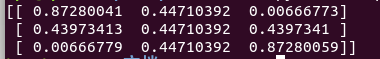
\includegraphics{./pic/chapter2/use_gpu1.png}\newline
\subsection{手工配置设备}
如果你想将你的操作运行在指定的设备中而不由tensorflow是自动为你选择,你可以用tf.device 创建一个设备,左右的操作将在同一个设备上指定。
\begin{python}
import tensorflow as tf
with tf.device('/cpu:0'):
    a = tf.constant([1.,2.,3.,4.,5.,6.],shape = (2,3),name = 'a')
    b = tf.reshape(a,shape=(3,2))
    c = tf.matmul(a,b)
    with tf.Session(config = tf.ConfigProto(log_device_placement=True)) as sess:
        print(sess.run(c))
\end{python}
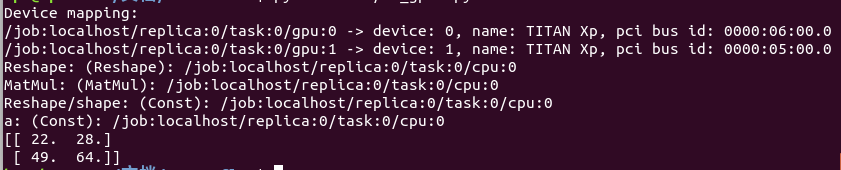
\includegraphics[scale=0.4]{use_gpu2.png}\newline
正如你看到的a,b被复制到cpu:0,因为设备没有明确指定,Tensorflow将选择操作和可用的设备(gpu:0)

\subsection{允许GPU的内存增长}

默认情况下Tensorflow将映射所有的CPUs的显存到进程上,用相对精确的GPU内存资源减少内存的碎片化会更高效。 通常有些程序希望分贝可用内存的一部分,或者增加内存的需要两。在会话中tensorflow提供了两个参数 控制它。 第一个参数是allow\_growth选项,根据运行情况分配GPU内存:它开始分配很少的内存,当Session开始运行 需要更多GPU内存是,我们同感Tensorflow程序扩展GPU的内存区域。注意我们不释放内存,因此这可能导致更多的内存碎片。为了开启这个选项,可以通过下面的设置
\begin{python}
config = tf.ConfigProto()
config.gpu_option.allow_growth = True
sess = tf.Session(config=config,...)
\end{python}
第二种方法是per\_process\_gpu\_memory\_fraction选项,决定GPU总体内存中多少应给被分配,例如你可以告诉 Tensorflow分配40\%的GPU总体内存。
\begin{python}
config = tf.ConfigProto()
config.gpu_option.per_process_gpu_memory_fraction = 0.4
sess = tf.Session(config = config)
\end{python}
如果你想限制Tensorflow程序的GPU使用量,这个参数是很有用的。

在多GPU系统是使用GPU

如果你的系统上有超过一个GPU,你的GPU的抵消的ID将被默认选中,如果你想运行在不同的GPU上,你需要指定 你想要执行运算的GPU
\begin{python}
import tensorflow as tf
with tf.device('/gpu2:0'):
    a = tf.constant([1.,2.,3.,4.,5.,6.],shape = (2,3),name = 'a')
    b = tf.reshape(a,shape=(3,2))
    c = tf.matmul(a,b)
    with tf.Session(config = tf.ConfigProto(log_device_placement=True)) as sess:
        print(sess.run(c))
\end{python}
如果你指定的设备不存在,你将个到一个InvalidArgumentError:\newline
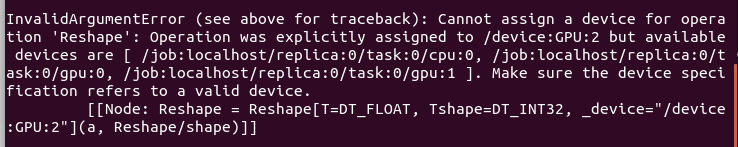
\includegraphics[scale=0.4]{use_gpu3.png}\newline
如果你想Tensorflow在万一指定的设备不存在时自动选择一个存在的设备,你可以在创建会话时配置中设置allow\_soft\_placement 为True
\begin{python}
with tf.device('/gpu:2'):
  a = tf.constant([1.,2.,3.,4.,5.,6.],shape= [3,2],name = 'a')
  b = tf.constant([1.,2.,3.,4.,5.,6.],shape= [2,3],name = 'b')
  c = tf.matmul(a,b)
with tf.Session(config = tf.ConfigProto(allow_soft_placement=True,log_device_placement=True)) as sess:
    print(sess.run(c))
\end{python}
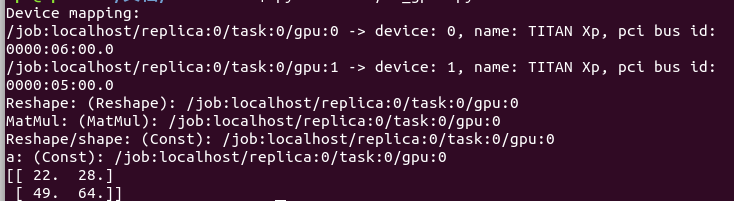
\includegraphics[scale=0.4]{use_gpu4.png}\newline
用多GPU

如果你想在多张GPU上运行Tensorflow,你可以在multi-tower fashion上构造你的模型,每个tower 被指定到不同的GPU上。例如:
\begin{python}
c = []
for d in ['/gpu:0', '/gpu:1']:
    with tf.device(d):
        a = tf.constant([1.0, 2.0, 3.0, 4.0, 5.0, 6.0], shape=[2, 3])
        b = tf.constant([1.0, 2.0, 3.0, 4.0, 5.0, 6.0], shape=[3, 2])
        c.append(tf.matmul(a, b))
    with tf.device('/cpu:0'):
        sum = tf.add_n(c)
   # Creates a session with log_device_placement set to True.
sess = tf.Session(config=tf.ConfigProto(allow_soft_placement=True,log_device_placement=True))
  # Runs the op.
print(sess.run(sum))
sess.close()
\end{python}
\section{如何利用Inception的最后一层重新训练新的分类}
现代的认知模型可能有上百万个参数可能需要花几周训练,Transfer学习是通过完整的像ImageNet一样的模型通过已经存在的权重简化数周工作分类的技术。在这个例子中我们将创新训练最终层不修改其它层。详细信息你可以查看\href{http://arxiv.org/pdf/1310.1531v1.pdf}{这篇论文}.

尽管不完整的训练,但是对于一些应用却惊人的高效,可以在笔记本上训练30分钟,不要求GPU。这个导航将显示给你如何在自己的图像运行示例脚本解释一些控制训练需要的脚本。
\subsection{训练花}
\begin{center}
\begin{figure}
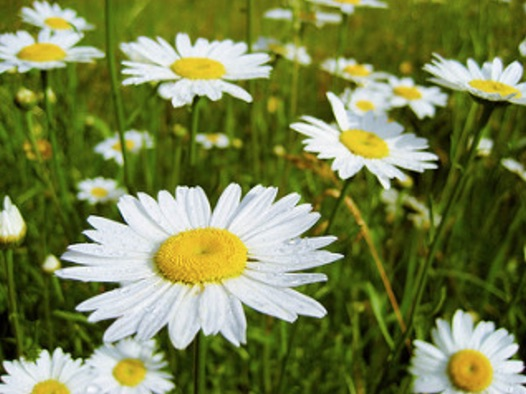
\includegraphics[scale=0.5]{daisies.jpg}
\end{figure}
\end{center}
在开始训练前你需要设置图像教网络你想认识的新的类别。接下来的张杰解释如何准备你的图像,但是我们创建一个授权的归档的花的文件使得训练更轻松。为了得到花的图像,运行下面的代码:
\begin{lstlisting}[language={[ANSI]C}]
cd ~
curl -O http://download.tensorflow.org/example_images/flower_photos.tgz
tar xzf flower_photos.tgz
\end{lstlisting}
当你有图像后,你从你的TensorFlow源文件目录构建重新训练器
\begin{lstlisting}[language={[ANSI]C}]
bazel build --config opt tensorflow/examples/image_retraining:retrain
\end{lstlisting}
可以通过下面运行:
\begin{lstlisting}{language=[ANSI]C}
bazel build tensorflow/examples/image_retraining:retrain
\end{lstlisting}
如果你有一个机器支持AVX设备集(最近几年的常用的x86 CPUs)你可以通过架构提高building运行速度
\begin{lstlisting}{language=[ANSI]C}
bazel build --config opt tensorflow/examples/image_retraining:retrain
\end{lstlisting}
训练器可以是这样:
\begin{lstlisting}{language=[ANSI]C}
bazel-bin/tensorflow/examples/image_retraining/retrain --image_dir ~/flower_photos
\end{lstlisting}
这个脚本载入先前incption v3模型,删除顶层,在新的flower photos训练新的模型。在原始ImageNet类中没有一种花完整网络被完整的训练过了,transfer学习是低层已经被训练好
区别不修改任何不同对象。
\subsection{瓶颈}
训练花费30分钟甚至更长时间取决于你的机器的速度。第一个时期分析所有磁盘上的图像和计算他们的瓶颈,瓶颈是一个信息对术语
我们经常在最后一层前一层,倒数第二层已经训练区别输出要求分类的值,这意味着这必须是有意义的,因此对于分类器它必须包含足够的信息在一些小的值得集合中做选择,这意味着我们的最终层训练可以在新的类中工作证明在ImageNet中1000类对于区别新的对象是有用的。
因为每个图像在训练和计算花费时间瓶颈时被多次使用,他的速度达到缓存起的瓶颈因此不能被重复计算。默认他们存储在/tmp/bottleneck陌路,如果你仍然会脚本他们将被重用,因此你不是必须再次等待这部分。
\subsection{训练}
当瓶颈计算完成时,实际顶层训练开始。你讲看到输出,显示精度,可用精度,交叉熵。训练精度显示在当前训练批中多少被分类正确,验证训练精度从图像数据集随机选中精度的值,不同之处在于训练精度基于网络已经学习到的参数,在训练中可能过拟合到为噪声。验证精确度用不在训练集中的数据性能测量精确度,如果训练精确度很高,测试精确度很低说明网络过拟合训练图像存储的部分参数没有用。交叉熵损失函数查看学习进程处理的增么样,训练对象使得损失尽可能小,因此你可以分辨出如果学习起作用,忽略损失噪声损失保持下降的趋势。默认脚本运行4000步,每一步从训练集中随机选择10张图像找到缓冲器的瓶颈,输入数据仅最终层预测。预测然后比较实际label和真实值差距反向传递误差。当你继续的时候你应该看到精确度的提高。你应该能看到精确度在90\%到95\%之间,通过提取值将随机的一次次训练,这个数完全训练好模型后基于在给定测试集中正确标签的百分比。
\subsection{用TensorBoard可视化}
包含TensorBaord总结的脚本吗很容易理解,调试,优化。例如,你可以可视化图和统计,例如在训练中权重和精度变化:
\begin{lstlisting}{language=[ANSI]C}
tensorbaord --logdir /tmp/retrain_logs
\end{lstlisting}
TensorBoard运行后导航到localhost:6006查看TensorBoard,脚本将默认采集TensorBoard总结到/tmp/retain\_logs,你可以通过summaries\_dir标志指定采集目录。
\subsection{用重新训练的模型}
脚本将用训练好的最后一层写出你的一个Inception v3版本到/tmp/output\_graph,text文件在/tmp/output\_labels.txt包含标签,两个格式见
\href{https://www.tensorflow.org/tutorials/image_recognition}{C++ and Python image classification examples},因此你可以立即开始新的模型。你去带最顶层,你将需要在脚本中指定新的名字,例如你用label\_image,用--outout\_layer=final\_result.
你可以用下面的代码重新训练图:
\begin{lstlisting}{language=[ANSI]C}
bazel build tensorflow/examples/image\_retraining:label\_image && \
bazel-bin/tensorflow/examples/image_retraining/label_image \
--graph=/tmp/output_graph.pb --labels=/tmp/output\_labels.txt \
--image=$Home/flower_photos/daisy/21625746_cc379eea_m.jpg
\end{lstlisting}
你应该看到花的标签的列表在大说书情况下daisy在顶层(尽管重新训练的模型被可能会一点不同),你可以用在你的图片上--image参数
用c++代码作为模板整合你自己的应用。
如果你想在自己的Python程序中用你训练好的模型,上面的\href{https://www.github.com/tensorflow/tensorflow/blob/r1.3/tensorflow/examples/image_retraining/label_image.py}{label\_image script}
如果你发现默认的Inception v3模型对你的应用太大或者太慢,看看\href{https://www.tensorflow.org/tutorials/image_retraining#other_model_architectures}{Other Model Architechtures section}
\subsection{在你自己的分类上训练}
如果你已经成功的让脚本在花的例子上工作,你可以教他认识其他你想它认识的东西。理论上你需要设置一个子文件夹,命名分类,每个文件夹包含分类的图像。如果你传递子文件夹的根文件夹作为参数给--image\_dir,脚本像上面训练花一样训练。
\begin{center}
\begin{figure}
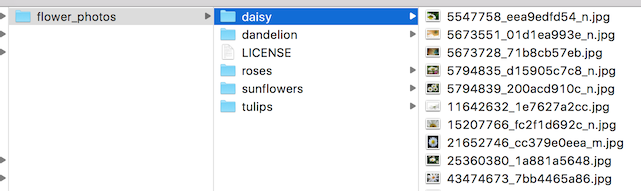
\includegraphics[scale=0.5]{folder_structure.png}
\end{figure}
\end{center}
实际上它会花一点时间得到你想要的精度,下面是一些常见的问题。
\subsection{创建一个训练图像集合}
首先我们需要查看收集到的图像,常见的问题是训练过程中数据的输入。

为了训练能起作用,每个你想要识别的图像你必须至少手机100张图片,你收集到的图片越多,训练的精确度可能越好。例如你拍摄一些蓝色的房间,另一些是绿色的房间模型的预测最终基于背景颜色,没有对象特征被考虑。为了避免这种情况,拍摄不同颜色的,没有一些实际能看到的的特征。如果你想了解更多这类问题你需要读\href{http://www.jefftk.com/p/detecting-tanks}{tank recognition}
如果你想考虑你用的分类。分隔大的数据集发现一些不同的物理形式为小的可以通过视觉区分的数据集,例如你可以用'vehicle'可以用来替代
'car','motobike'和'truck',考虑你有一个开放的世界还是封闭的世界将是很有价值的,在封闭的世界你唯一需要考虑的是识别已有的对象,例如一个植物识别的app你应该知道用户可能拍摄的花的图片,英雌你必须决定花的种类,相比之下一个巡逻机器人可能通过摄像头看到不同的事物。在这种情况下你想要分类器报告是否确认他看到的,这可能很难,但是你经常收集一些典型的和主体对象不相关的背景图像,,你可能会让它增加一些图片文件夹中未知的分类。
检查确保你的图像被正确的标记也是很重要的。经常用生成的标签对于你的目的来说是不可靠的,例如你用\#daisy命名一个叫Daisy的人。如果你想你的图像如果你了解你的图像,扫除任何错误将可能导致最后精确度提高。
\subsection{训练步骤}
如果你为你的图片感到高兴,你可以通过修改学习进程中的细节提升你的结果。最简单的方法是用--how\_many\_training\_steps。默认是4000.但是如果你增加到8000,他的训练时间将增加到两倍。精确度提高的比率显示你训练的越长一些点将停止,但是你可以试验什么时候达到你的模型的限制。
\subsection{扭曲}
随机通过变形,剪裁,变化输入图像的亮度是一个提高结果的常用方法,这样扩展了训练数据的大小,帮助网络学习
真是生活分类器所有的扭曲,在脚本中使用扭曲最大的缺点是缓冲瓶颈不再有用,因此输入图像将不能重用。这意味着训练京城可能花费更多时间,因此我推荐当着作为一个调节方法调节你的模型到合理。
你可以传递--random\_corp,--random\_scale和--random\_brightness给脚本扭曲图片。百分比值用来控制图片上扭曲用多少部分。,合理的值时5或者10.--flip\_left\_right将在水平方向随机的镜像图像的一半,有助有你的应用能理解翻转的图像。例如如果你想识别字母这将不是一个好的办法,因为翻转它们会毁掉原来的含义。
\subsection{超参数}
你可以调整一些参数查看是否对你的结果有帮助,--learning\_rate控制最终层训练更新的幅度。直观理解,如果这个值变小训练时间将边长,但是他可能对精度有帮助,你需要小心试验得到查看什么对于你的case生效了。--train\_batch\_size控制每一训练步多少图像被检查,因为学习率应用到每批上,如果你有更大的批得到相同的效果你将需要减小它。
\subsection{训练,验证,测试集}
当你为你的脚本指定图像文件夹时,文件夹被分成不同的数据集。最大的数据及是训练集,训练集包含用于训练网络的数据,用于更新权重。你也许很想知道为什么我们不用所有的图像训练?一个道德潜在的问题是当我们做机器学习算法时我们的模型会记住接近正确答案的不相关信息,你可以想想你的图像可能记住了一些照片的背景,通过标签匹配对象,它在训练时所有的图像可能产生一个好的结果,但是不能再新的图像产生好的结果因为他不能泛化对象的特征,仅仅在训练图像的时候记住了一些不重要的特征。
这个问题被称为过拟合,为了避免过拟合我们保持我们的一些数据不再训练进程中,因此模型不能记住他们,我们用这些图像作为检察确保过拟合没有发生,当我们在看模型在这些数据上有一个好的精度说明过拟合没有发生,通常80\%的数据被用来作为训练集10\%的数据集用来验证最后10\%的数据用做测试集预测分类器在真实世界的性能,通过--testing\_percentage和--validation\_percentage标志用来控制比例。通常你应该能留下一些值作为默认,不应该找到任何好处训练调整他们。
注意这个脚本用图象的文件名区分训练集,验证集,测试集中的图像(不是一个随机的函数),这样保证运行时图片不会再训练集和测试集之间移动,因为当用于训练模型的图像被验证集中的图像取代时可能会出现一些问题。
你也需注意到了在迭代过程中验证正确度的波动。多数波动是验证集的子集的随机性引起的,选择的验证集用来验证精确度。波动能能被最大层度减少,花费的训练时间增长,通过选择--validation\_batch\_size=-1用整个验证集计算精度。
当训练结束后你将能检查测试集中错误分类图像,这可以通过增加--print\_misclassified\_test\_images标记,这对于找到那些什么类型的图片让模型困惑(很难区别的)是很有帮助的例如你也许发现了一些种类一些常见的图像角度是特别难是别的,这样是鼓励你增加更多类型的分类训练子类,检查催哦五分类图片也指出输入数据中的错误,向错误标签,其质量魔术的照片。然而,你应该避免测试集固定点单个误差,因为他们仅仅反映在训练集中更多的问题。
\subsection{更对模型架构}
这个脚本默认用Inception v3模型架构作为预先训练脚本。这是一个好的开始的地方,因为它提供了高精度的训练结果,但是如果你想部署你的模型到手机设备或者其他的资源限制的环境你也许想要这种精确度换区更小的文件尺寸和更快的速度。
为了帮助这个\href{https://github.com/tensorflow/tensorflow/blob/master/tensorflow/examples/image_retraining/retrain.py}{retrain}
在\href{https://research.googleblog.com/2017/06/mobilenets-open-source-models-for.html}{移动架构}上支持30个不同的变量。
这里有一些比Inception v3更小精度的,但是可以得到更小的文件大小(下载小于兆字节)运行快乐几倍。为了训练这个模型,传递--architecture标志,例如:
\begin{lstlisting}{language={ANSI}C}
python tensorflow/examples/image_retraining/retrain.py \
    --image_dir ~/flower_photos -- architecture mobilenet_0.25_128_quantized
\end{lstlisting}
这将在/temp/创建一个941KB模型文件output\_graphi.pb.Mobilenet的25\%的参数,占据$128\times128$大小的输入图像,权重在磁盘中量化为8位,你可以选择'1.0','0.75','0.50','0.25'控制权重参数的数量,因此文件尺寸(和一些扩展速度),'224','192','160'或者'128'对于输入图像的尺寸,更小的尺寸更快的速度,选项'\_quantized'预示着是否文件应该包含8位或者32位浮点权重。速度和大小好处带来的是精确度的损失,但是对于一些用途来说是不重要的,他可以通过训练数据提高、例如用扭曲在花数据集允许你得到得到80\%的精度,甚至0.25/128、quantized图。
如果你在你的程序或者label\_image中用Mobilenet模型,你讲需要一个输入一个指定大小的图像转换一个浮点让位到'input' tensor,典型的24位乳香范围[0,255]你必须用(image-128.)/128转化它到[-1,1]范围。
\section{TF layer想到:建立一个卷积神经网络}
TensorFlow\href{https://www.tensorflow.org/api_docs/python/tf/layers}{layers module}是一个用于轻松建立神经网络的高级API,它提供了一个方法促进创建dense(全连接)层和卷积层,增加激活函数,应用dropout规则。在这个导航中,你讲学习如何用layers建立一个卷积神经网络模型识别手写体数据集。
\textbf{手写体数据集包含0-9,60000个训练样本10000个测试样本,图像格式为}$28\times28$
\subsection{开始}
创建文件cnn\_mnist.py,在手写体程序中添加如下代码:
\begin{python}
from __future__ import absolute_import
from __future__ import division
from __future__ import print_function

# Imports
import numpy as np
import tensorflow as tf

tf.logging.set_verbosity(tf.logging.INFO)

# Our application logic will be added here

if __name__ == "__main__":
  tf.app.run()
\end{python}
正如你看到的,你讲增加到吗构造,训练,评估卷积神经网络,最终代码可以点击\href{https://www.github.com/tensorflow/tensorflow/blob/r1.3/tensorflow/examples/tutorials/layers/cnn_mnist.py}{这里}
\subsection{介绍卷积神经网络}
卷积神经网络是当前最先进的用于图像分类任务的模型架构。CNNsCNNs应用一些滤波器从原始的图像像素中提取高级特征,这个模型可能被用在分类。CNN包含三个组件:
\begin{itemize}
  \item \textbf{卷积层} 应用指定数量的卷积滤波器在图像上。对于每一个子区域,layer执行一系列数学操作生成一个单个值在输出feature map,卷积层然后应用relu激活函数输出非线性。
  \item \textbf{池化层} 下采样卷积层的图像数据,减小feature map的维度从而减小处理时间。常用池化算法是最大池化(提取feature map子区域)保留最大值,丢掉其它值。
  \item \textbf{Dense layers(全连接层)}在通过卷积层和下采样层特征提取执行分类。在全连接层,每一个节点连接到前面的节点。
\end{itemize}
通常CNN有一个卷积模块组成,每个层有卷积模块和池化模块组成。最新的卷积模块有一个或者更多的全连接层链接执行分类。最终CNN的全连接层包含每个目标类的一个单个节点(所有模型可能预测的类),用sofymax函数生成一个0-1的值(所有值的和维1)。我们可以解释给定图像和目标的相似情况。
\subsection{建立CNN MNIST分类器}
用CNN架构建立模型分类MNIST数据集。
\begin{enumerate}
  \item 卷积层:应用
\end{enumerate}

{常用的python模块}
\section{Argparse}
argparse模块是一个用户用户友好的命令行接口,当用户每有给定可用的参数时,argaprser能自动生成帮助和使用信息。
\begin{python}
import argparse
parser = argparse.ArgumentParser(description='Process some integers.')
parser.add_argument('integers',metavar='N',type=int,nargs='+',help='an integer for the accumulator')
parser.add_argument('--sum',dest='accumulate',action='store_const',const=sum,default=max,help='sum the integers(default:find the max)')
args = parser.parse_args()
print(args.accumulate(args.integers))
\end{python}
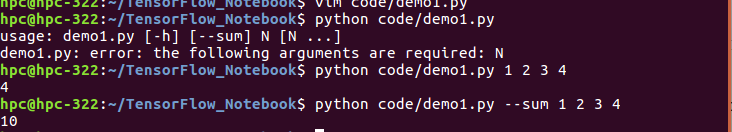
\includegraphics[scale=0.5]{demo1.png}\newline

代码能根据传入的参数选择相应的函数计算。
\begin{itemize}
\item 创建一个parser
\item 增加arguments
\item 解析参数
\end{itemize}

\subsection{ArgumentParser 对象}
class argparse.ArgumentParser(prog=None, usage=None, description=None, epilog=None, parents=[], formatter\_class=argparse.HelpFormatter, prefix\_chars='-', fromfile\_prefix\_chars=None, argument\_default=None, conflict\_handler='error', add\_help=True, allow\_abbrev=True)
\begin{itemize}
\item prog:程序的名字(默认为sys.argv[0])
\item usage:描述程序用法的字符串。(默认同感arguments增加到parser)
\item description:argument帮助前的文本展示。(默认为:None)
\item epilog:argument帮助之后的文本展示。(默认为:None)
\item parents:应该被包含的列表对象。
\item formatter\_class:自定义输出帮助的类。
\item prefix\_chars:参数前面的字符。(默认为'-')
\item fromfile\_prefix\_chars:应该被读的文件的字符串。
\item argument\_default:参数的全局值。(default:None)
\item conflict\_handler:解决冲突选项的策略。(通常不是必需的)
\item add\_help:增加-h/--help选项到parser。(默认为True)
\item allow\_abbrev:如果缩略不冲突,可以允许长的选项被缩略。(默认为True)
\end{itemize}
\subsection{prog}
默认情况下ArgumentParser对象用sys.argv[0]决定如何显示程序的名字。
\begin{python}
#filename:arg1.py
import argparse
parser = argparse.ArgumentParser()
parser.add_argument("echo")
args = parser.parse_args()
print(args.echo)
\end{python}
默认情况下ArgumentParser从包含用法信息的参数计算useage message。
\begin{python}
import argparse
parser = argparse.ArgumentParser()
parser.add_argument('--foo',help='foo help')
args = parser.parse_args()
\end{python}

\begin{figure}[htbp]
\centering
\subfigure[name of the subfigure]{
\begin{minipage}{5cm}
\centering
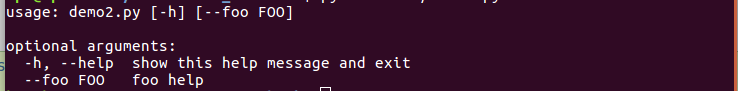
\includegraphics[scale=0.5]{demo2.png}
\end{minipage}}
\subfigure[name of the subfigure]{ 
\begin{minipage}{5cm}
\centering
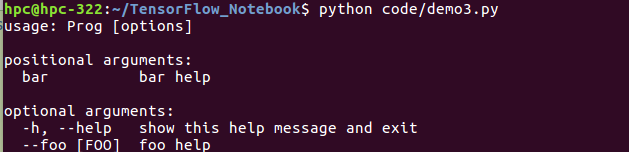
\includegraphics[scale=0.3]{demo3.png}
\end{minipage}}
\label{fig:1}
\end{figure}
大多数的ArgumentParser构造体用description=关键字,这个参数给出一个简单的程序说明其如何工作的。在帮助信息中表述在命令行和帮助信息之间。
\begin{python}
import argparse
parser = argparse.ArgumentParser(description='A foo that bars')
parser.print_help()
\end{python}
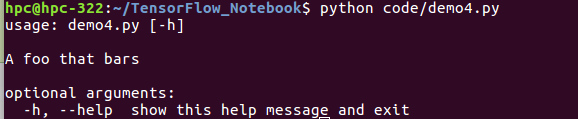
\includegraphics[scale=0.5]{demo4.png}\newline
一些程序喜欢在参数表述后添加一些额外的信息说明,这些说明可以同感ArgumentParser中的epilog=参数指定。
\begin{python}
import argparse
parser = argparse.ArgumentParser(description='A foo that bars',
epilog="And that's how you'd foo a bar")
parser.print_help()
\end{python}
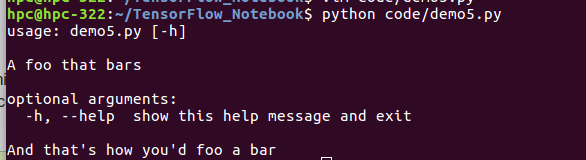
\includegraphics[scale=0.5]{demo5.png}
有时候一些parser共享一些参数,相比于重复定义这些参数,一个单个的parser同感传递parents给ArgumentParser。parents=参数得到一个ArgumentParser对象的列表对象,从中收集所有的位置和选项行为\newline
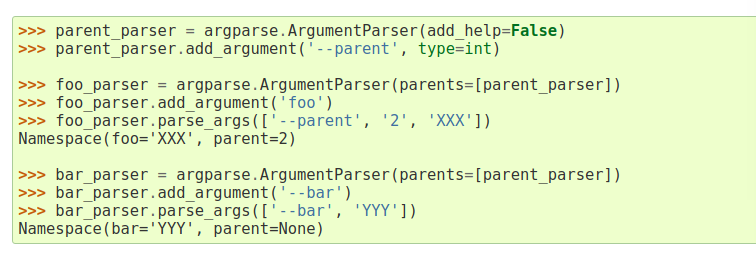
\includegraphics[scale=0.4]{demo6.png}\newline
大多数的parent parser指定add\_help=False,因此ArgumentParser将看到两个帮助选项(一个在parent一个在child)同时报错。你必须在通过parsers=传递前必须完全初始化parser,如果你在child parser改变parent parsers,改变将不被反映到child。
formatter\_class
ArgumentParserdurian允许指定可用的格式化类自定义格式,当前有4个类:
\begin{itemize}
\item argparse.RawDescriptionHelpFormatter
\item argparse.RawTextHelpFormatter
\item argparse.ArgumentDefaultHelpFormatter
\item argparse.MetavarTypeHelpFormatter
\end{itemize}

RawDescriptionHelpFormatter和RawTextHelpFormatter在如何显示说明上给与更多控制,默认ArgumentParser对description和epilog在命令终端一行显示。
\begin{python}
import argparse
parser = argparse.ArgumentParser(prog='PROG',description='''this
 description was indented wierd
but that is okey''',
epilog='''
likewise for this epilog whose whitespace will be
cleaned up and whose words will be wrapped
across a couple lines''')
parser.print_help()
\end{python}
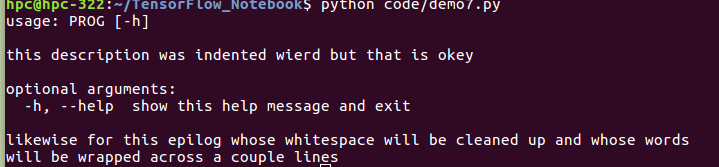
\includegraphics[scale=0.5]{demo7.png}\newline
传递RawDescriptionHelpFormatter作为formatter\_class=让description和epilog正确显示。
RawTextHelpFormatter主要维持素有的帮助文本,值描述的信息。\newline
ArgumentDefaultHelpFormatter:自动增加关于值的默认信息。\newline
\begin{python}
import argparse
parser = argparse.ArgumentParser(prog='Prog',
formatter_class = argparse.ArgumentDefaultsHelpFormatter)
parser.add_argument('--foo',type=int,default=42,help='FOO')
parser.add_argument('bar',nargs='*',default=[1,2,3],help='BAR!')
parser.print_help()
\end{python}
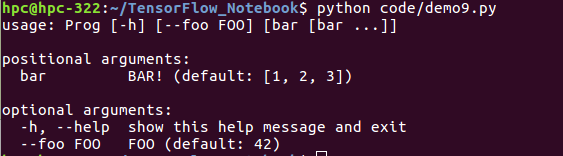
\includegraphics[scale=0.5]{demo8.png}
MatavarTypeHelpFormatter用type显示参数显示值的名字。
\begin{python}
import argparse
parser = argparse.ArgumentParser(prog='Prog',
formatter_class = argparse.ArgumentDefaultsHelpFormatter)
parser.add_argument('--foo',type=int,default=42,help='FOO')
parser.add_argument('bar',nargs='*',default=[1,2,3],help='BAR!')
parser.print_help()
\end{python}
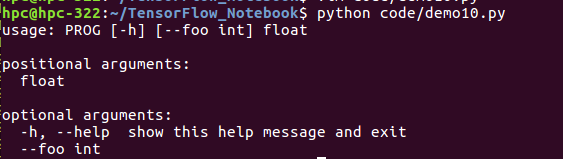
\includegraphics[scale=0.5]{demo9.png}\newline
prefix\_chars,大多数命令行参数选项用-,比如-f/--foo。parsers需要支持不同的或者说另外的前缀,像+f或者/foo
就可以设置prefix\_chars=参数指定。prefix\_chars默认默认为-,用非-字符能禁用-f/--foo这种类型性的选项。\newline
\begin{python}
import argparse
parser = argparse.ArgumentParser(prog='PROG',prefix_chars='-+')
parser.add_argument('+f')
parser.add_argument('++bar')
parser.parse_args('+f X ++bar Y'.split())

\end{python}
fromfile\_prefix\_chars,有时我们处理一个长的参数列表,将参数保存在文件中比直接在命令行中更容易理解,如果fromfile\_prefix\_chars=参数给ArgumentParse结构体,指定的参数将被作为文件,被下面的参数取代。例如
\begin{python}
import argparse
with open('args.txt','w') as fp:
    fp.write('-f\nbar')
parser = argparse.ArgumentParser(fromfile_prefix_chars='@')
parser.add_argument('-f')
parser.parse_args(['-f','foo','@args.txt'])
\end{python}
默认从一个文件读取参数,上面的表达式['-f','foo','@args.txt']等于表达式['-f','foo','-f','bar'],fromfile\_prefix\_chars参数默认为None,意味着参数不被当作文件。
argument\_default\par
通常通过传递add\_argument或者通过调用set\_defaults()方法指定名字和值对,然而有时候通过给参数指定一个简单的parser-wide是有用的,这可以通过传递argument\_default=关键字到ArgumentParser,例如调用其全局抑制属性在parse\_args()调用,我们用argument\_default=SUPPRESS:
\begin{python}
import argparse
parser = argparse.ArgumentParser(argument_default=argparse.SUPPRESS)
parser.add_argument('--foo')
parser.add_argument('bar',nargs='?')
parser.parse_args(['--foo','1','BAR'])
print(parser.parse_args([]))
\end{python}
allow\_abbrev\par
通常我们传递一个参数liebhiao给ArgumentParser的方法parse\_args(),如果选项参数太长的话。特征展示可能通过设置allow\_abbrev设置为False被禁用。
\begin{python}
import argparse
parser = argparse.ArgumentParser(prog='Prog',allow_abbrev=False)
parser.add_argument('--foobar',action='store_true')
parser.add_argument('--fooley',action='store_true')
parser.parse_args(['--foon'])
\end{python}
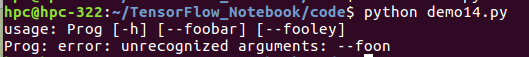
\includegraphics[scale=0.5]{demo10.png}\newline
conflict\_handler\newline
ArgumentParser对象不允许相同的选项字符串有两个行为,默认情况下当已经一偶选项字符串使用时尝试穿件一个新的参数ArgumentParser对象将报出异常。
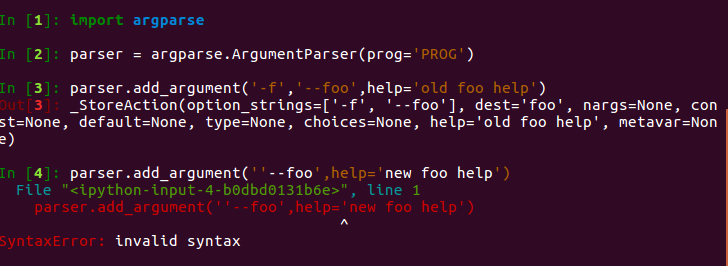
\includegraphics[scale=0.5]{demo11.png}
有时候覆盖掉就得参数时有用的,为了得到参数的行为值'resolcve'可能被应用在conflict\_handler=参数。
\begin{python}
import argparse
parser = argparse.ArgumentParser(prog='PROG',conflict_handler='resolve')
parser.add_argument('-f','--foo',help='old foo help')
parser.add_argument('--foo',help='new foo help')
parser.print_help()
\end{python}
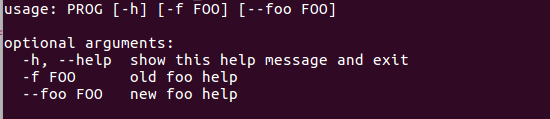
\includegraphics[scale=0.5]{demo12.png}\newline
如果所有的选项字符串被覆盖,ArgumentParser对象仅仅移除一个行为,因此上面的例子中,就得行为-f/--foo行为保留-f行为,因为仅仅--foo选项字符串被覆盖。
add\_help\par
默认情况下ArgumentParserdurian增加帮助信息到显示的消息中,例如:
\begin{python}
import argparse
parser = argparse.ArgumentParser(description='Process some integers.')
parser.add_argument('integers',metavar='N',type=int,nargs='+',help='an integer for the accumulator')
parser.add_argument('--sum',dest='accumulate',action='store_const',const=sum,default=max,help='sum the integers(default:find the max)')
args = parser.parse_args()
print(args.accumulate(args.integers))
\end{python}
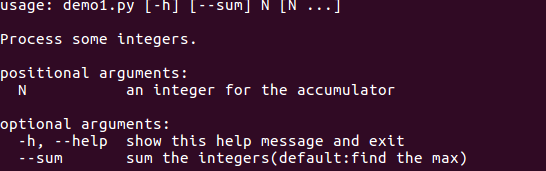
\includegraphics[scale=0.5]{demo13.png}
\begin{python}
import argparse
parser = argparse.ArgumentParser(description='Process some integers.',add_help=False)
parser.add_argument('integers',metavar='N',type=int,nargs='+',help='an integer for the accumulator')
parser.add_argument('--sum',dest='accumulate',action='store_const',const=sum,default=max,help='sum the integers(default:find the max)')
args = parser.parse_args()
print(args.accumulate(args.integers))
\end{python}
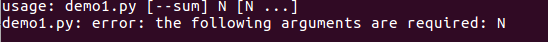
\includegraphics[scale=0.5]{demo14.png}
\subsection{add\_argument()方法}
ArgumentParser.add\_argument(name or flags...[, action][, nargs][, const][, default][, type][, choices][, required][, help][, metavar][, dest])
定一个一个命令行参数应该被如何解析,每一个参数自己有自己的详细描述,如下:
\begin{itemize}
\item name or flags:名字或者选项字符串,foo或者(-f,--foo)。
\item action:参数出现在命令行后采取的基本的行为。
\item nargs:命令行参数应该被使用的参数的数量。
\item const:action和nargs选项要求的常数值。
\item default:缺乏参数的默认值。
\item type:传递参数读额数据类型。
\item choices:参数的允许值的容器。
\item required:是否命令行选项被乎略。
\item help:简易的参数说明。
\item metavar:在usage消息的名字。
\item dest:增加到parse\_args()返回对象的属性的名字。
\end{itemize}
name或者flags\par
当parse\_args()被调用的时候。选项参数通过-前缀识别。
\begin{python}
import argparse
parser = argparse.ArgumentParser(prog='PROG')
parser.add_argument('-f','--foo')
parser.add_argument('bar')
print(parser.parse_args(['BAR']))
print(parser.parse_args(['BAR','--foo','FOO']))
\end{python}
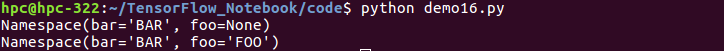
\includegraphics[scale=0.5]{demo15.png}
action\par
\begin{itemize}
\item 'store':仅仅保存参数的值,例如
\begin{python}
parser = argparse.ArgumentParser()
parser.add_argument('--foo')
parser.parse_args('--foo 1'.split)
\end{python}
输出Namespace(foo='1')\par
\item 'store\_true':存储const参数指定的值,'store\_const'行为通常用于指定一些flag。
\begin{python}
parser = argparse.ArgumentParser()
parser.add_argument('--foo',action='store_contt',const=42)
parser.add_argument('--foo')
\end{python}
输出:Namescpae(foo=42)
\item 'store\_true'和'store\_false'指定'store\_const'。
\begin{python}
parser = argparse.ArgumentParser()
parser.add_argument('--foo',action='store_true')
parser.add_argument('--bar',action='store_false')
parser.add_argument('--baz',action='store_false')
parser.parse_args('--foo --bar'.split())
\end{python}
输出:Namespace(foo=True,abr=False,baz=True)
\item 'append':一个存储列表,添加每个参数值到列表中,允许选项被多次指定时很有用。
\begin{python}
parser = argparse.ArgumentParser()
parser.add_argument('--str',dest='types',action='append_const',const=str)
parser.add_argument('--int',dest='types',action='append_const',const=int)
parser.parse_args('--str --int'.split())
\end{python}
输出:Namespace(type=[<class 'str'>,<class 'int'>])
\item 'count':关键参数出现的次数。
\begin{python}
parser = argparse.ArgumentParser()
parser.add_argument('--verbose','-v',action='count')
parser.parse_args(['-vvv'])
\end{python}
输出:Namespace(varbose=3)
\item help:打印当前parser所有选项的帮助信息,默认帮助行为被添加到parser。
\item version:add\_argument调用指定version=关键字
\begin{python}
import argparse
parser = argparse.ArgumentParser(prog='PROG')
parser.add_argument('--version',action='versddion',version='(%prog)s 2.0')
parser.parse_args(['--version'])
\end{python}
输出PROG 2.0。
\item 你可以同感传递行为子类或者其它对象的接口传递给action,推荐的方法是扩展Action,覆盖掉\_\_call\_\_方法和\_\_init\_\_。
\begin{python}
class FooAction(argparse.Action):
    def __init__(self,option_strings,dest,nargs=None,**kwargs):
        if nargs is not None:
            raise ValueError("nargs not allowed")
    def __call__(self,parser,namespace,values,option_string=None):
        print('%r%r%r'%(namespace,values,option_string))
        setattr(namespace,self.dest,values)
parser = argparse.ArgumentParser()
parser.add_argument('--foo',action=FooAction)
parser.add_argumentParser('bar',action=FooAction)
args = parser.parse_args('1 -- foo 2'.split)
\end{python}
\end{itemize}
输出:\newline
Namespace(bar=None,foo=None) '1' None\newline
Namespace(bar=1,foo=None) '2' '--foo' \newline
nargs\newline
\begin{itemize}
\item N:一个整数,命令行下的参数被放到一起成为一个列表:
\begin{python}
parser = argparse.ArgumentParser()
parser.add_argument('--foo',nargs=2)
parser.add_argument('bar',nargs=1)
parser.parse_args('c --foo a b'.split())
\end{python}
输出:Namespace(bar=['c'],foo=['a','b'])
\item ?:根部不同情况生成不同的值,如果没有参数指定它的值来自默认生成如果有一个带有-前缀的参数值将被const参数生成,如果指定了值将生成指定值。
\begin{python}
parser = argparse.ArgumentParser()
parser.add_argument('--foo',nargs='?',const='c',default='d')
parser.add_argument('bar',nargs='?',default='d')
parser.parse_args(['XX','--foo','YY'])
parser.parse_args(['XX','--foo'])
parser.parse_args([])
\end{python}
分别输出:\newline
Namespace(bar='XX',foo='YY')\newline
Namespace(bar='XX',foo='x')\newline
Namespace(bar='d',foo='d')\newline
用nargs='?'更常用的用法时允许选项输入输出文件:
\begin{python}
parser = argparse.ArgumentParser()
parser.add_argument('infile',nargs='?',type=argparse.FileType('r'),default=sys.stdin)
parser.add_argument('outfile',nargs='?',type=argparse.FileType('w'),default=sys.stdout)
parser.parse_args(['input.txt','output.txt'])
\end{python}
输出:Namespace(infile=<\_io.TextIOWrapper name='input.txt',encoding='UTF-8'>,
outfile<\_io.TextIOWrapper name='output.txt' encoding='UTF-8'>)
parser.parse\_args([])
输出:
Namespace(infile=<io.TextIOWrapper name='<stdin>' encoding='UTF-8'>,
outfile=<\_io.TextIOWrapper name='<stdout>' encoding='UTF-8'>)
\item *:所有的命令行参数将被放到一个列表中。
\begin{python}
parser = argparse.ArgumentParser()
parser.add_argument('--foo',nargs='*')
parser.add_argument('--bar',nargs='*')
parser.add_argument('--barz',nargs='*')
parser.parse_args('a b --foo x y --bar 1 2'.split())

\end{python}
输出:Namespace(bar=['1','2'],baz=['a','b'],foo=['x','y'])
\item +:所有的命令行参数将被添加到一个列表中,至少需要一个参数肉则将报错。
\begin{python}
parser = argparse.ArgumentParser(prog='PROG')
parser.add_argument('foo',nargs='+')
parser.parse_args(['a','b'])
parser.parse_args([])
\end{python}
输出:Namespace(foo=['a',nargs='+'])\newline
usage: PROG [-h] foo [foo ...]\newline
PROG: error: too few arguments\newline
\item argparse.REMAINDER:所有已经存在的参数被添加到一个列表。
\begin{python}
parser = argparse.ArgumentParser(prog='PROG')
parser.add_argument('--foo')
parser.add_argument('command')
parser.add_argument('args',nargs=argparse.REMAINDER)
print(parser.parse_args('--foo B cmd --arg1 xx zz'.split()))
\end{python}
输出:Namespace(args=['--arg1','XX','ZZ'],command='cmd',foo='B')
如果nargs参数没有提供,argument 由action决定,通常这意味着一个的命令行参数被使用一个项目被产生。
\end{itemize}
const\par
const参数被用在保存没有被命令行读入的常数来常数值,两个常见的用法如下:
\begin{itemize}
\item 当add\_argument()调用的时候设置了action='store\_const'或者是action='append\_cost'同感增加const值到一个parse\_args()返回的对象的属性。
\item 当add\_argument()通过选项字符串(像-f或者--foo)和nargs='?',这将穿件一个由0行或者一行参数跟着的选项,当解析命令行时,如果选项字符串遇到没有命令行参数的时候,值const将被用来替代。'store\_const'和'append\_const'行为,const关键字参数必须给定,对于其它行为,默认为None。
\end{itemize}
default\par
所有的参数和一些位置的参数在命令行下可能被忽略,add\_argument()参数default的值默认为None,指定当没有参数时什么值被使用。没有指定选项字符串,default的值将取代参数。
\begin{python}
parser = argparse.ArgumentParser()
parser.add_argument('--foo',default=42)
parser.parser_args(['--foo','2'])
parser.parse_args([])
\end{python}
输出:
Namespace(foo='2')\newline
Namespace(foo=42)\newline
如果默认值是一个字符串,parser解析值就好象命令行参数一样,类似的,parser应用任何type转换参数,如果在设置属性值前Namespace返回值,否则parser用下面的值。
\begin{python}
parser = argparse.ArgumentParser()
parser.add_argument('--length',default=42,type=int)
parser.add_argument('--width',default=10.5,type=int)
parser.parse_args()
\end{python}
输出:Namesapce(length=10,width=10.5)\newline
对于参数为'?'或者'*',命令行没有值的时候default值将被使用
\begin{python}
parser = argparse.ArgumentParser()
parser.add_argument('foo',nargs='?',default=42)
parser.parse_args(['a'])
parser.parse_args([])
\end{python}
分别输出:\newline
Namespace(foo='a')\newline
Namespace(foo=42)\newline
如果default=argparse.SUPPRESS如果没有命令行参数将导致没有属性被添加。
\begin{python}
parser = argparse.ArgumentParser()
parser.add_argument('--foo',default=argparse.SUPPRESS)
parser.parse_args([])
parser.parse_args(['--foo','1'])
\end{python}
分别输出:\newline
Namespace()\newline
Namespace(foo='1')\newline
type\par
默认ArgumentParser对象读命令行参数为字符串,然而,经常命令行应该以另一种数据类型解析,像float,int,add\_argument()的type关键字允许需要的类型检查和转换被执行,常用的内部数据类型和参数可以被作为type的值直接使用。
\begin{python}
parser = argparse.ArgumentParser()
parser.add_argument('foo',type=int)
parser.add_argument('bar',type=open)
parser.parse_args('2 temp.txt'.split())
\end{python}
输出:Namespace(bar=<\_io.TextIOWrapper name='temp.txt' encoding='UTF-8',foo=2)
为了能轻松的使用多种文件类型,argparse模块提供了工厂FileType,利用mode=,bufsize=,encoding=和error=参数,例如FileType('w')可以被用来创建一个可写的文件。
\begin{python}
parser = argparse.ArgumentParser()
parser.add_argument('bar',type=argparse.FileType('w'))
parser.parse_args(['output'])
\end{python}
输出:Namespace(bar=<\_io.TextIOWrapepr name='out.txt' encoding=;UTF-8;>)
type能够调用一个字符串参数返回转换过值的参数
\begin{python}
import math
import argparse
def perfect_square(string):
    value = int(string)
    sqrt = math.sqrt(value)
    if sqrt!=int(sqrt):
        msg='%r is not a perfect square'%string
        raise argparse.ArgumentTypeError(msg)
    return value
parser = argparse.ArgumentParser(prog='PROG')
parser.add_argument('foo',type=perfect_square)
print(parser.parse_args(['9']))
print(parser.parse_args(['7']))

\end{python}
输出:
Namespace(foo=9)\newline
usage: PROG [-h] foo\newline
PROG: error: argument foo: '7' is not a perfect square\newline
choise\par
choise参数在检查值的范围时很方便。
\begin{python}
parser = argaprse.ArgumentParser(prog='PROG')
parser.add_argument('foo',type=int,choice=range(5,10))
parser.parse_args(['7'])
parser.parse_args(['11'])
\end{python}
分别输出:Namespace(foo=7)\newline
usage: PROG [-h] {5,6,7,8,9}\newline
PROG: error: argument foo: invalid choice: 11 (choose from 5, 6, 7, 8, 9)\newline
choise\par
一些命令行参数从一些限定值的中选定,可以通过传递choice关键字参数给add\_argument(),当命令行解析的时候,值将被检查如果不在可接受值范围内将显示错误消息。
\begin{python}
parser = argparse.ArgumentParser(prof='game.py')
parser.add_argument('move',choices=['rock','paper','scissors'])
parser.parse_args(['rock'])
parser.parse_args(['file'])
\end{python}
分别输出:\newline
Namespace(move='rock')\newline
usage: game.py [-h] {rock,paper,scissors}\newline
game.py: error: argument move: invalid choice: 'fire' (choose from 'rock',
'paper', 'scissors'\newline
choice选项检查在转化数据类型后进行。
\begin{python}
parser = argparse.ArgumentParser(prog='doors.py')
parser.add_argument('door',type=int,choices=range(1,4))
print(parse.parse_args(['3']))
print(parser.parse_args(['4']))
\end{python}
分别输出:\newline
Namespace(door=3)\newline
usage: doors.py [-h] {1,2,3}\newline
doors.py: error: argument door: invalid choice: 4 (choose from 1, 2, 3)\newline
任何支持in操作的对象都能被传递给choise作为值,因此dict,set对象都是常用的支持的对象。
required\par
通常argparse模块假设flag像可以被省略的-f和--bar,,为了一个选项必需要需要设置required=True。
\begin{python}
parser = argparse.ArgumentParser()
parser.add_argument('--foo',required=True)
parser.parse_args(['--foo','BAR'])
parer.parse_args([])
\end{python}
分别输出:\newline
Namespace(foo='BAR')\newline
usage: argparse.py [-h] [--foo FOO]\newline
argparse.py: error: option --foo is required\newline
正如上例,如果parse\_args()的required被标记,如果不给值将报错。
help\par
help值包含一些简单的参数说明,当用户要求帮助的时候(通常用-h或者--help),help描述信息将被展示
\begin{python}
parser = argparse.ArgumentParser(prog='frobble')
parser.add_argument('--foo',action='store_true',help='foo the bars before frobbing')
parser.add_argument('bar',nargs='+',help='foo the bars before frobbed')
parser.parse_args(['-h'])
\end{python}
输出:\newline
usage: frobble [-h] [--foo] bar [bar ...]\newline
positional arguments:\newline
 bar     one of the bars to be frobbled\newline

optional arguments:\newline
 -h, --help  show this help message and exit\newline
 --foo   foo the bars before frobbling\newline
help字符串能包含多种格式像程序名字或者默认参数,可用的指定包含程序的名字,\%(prog)s和多数add\_argument()关键字,像\%(default)s,\%(type)s等等。
\begin{python}
parser = argparse.ArgumentParser(prog='frobble')
parser.add_argument('bar',nargs='?',type=int,default=42,help='the bar to %(prog)s(default:%(default)s)')
parser.print_help()
\end{python}
输出:\newline
usage: frobble [-h] [bar]\newline

positional arguments:\newline
 bar     the bar to frobble (default: 42)\newline

optional arguments:\newline
 -h, --help  show this help message and exit\newline
帮助字符串支持\%格式,如果你想一个\%出现在帮助字符串中,你需要使用\%\%
argparse对于指定的选项通过设置argparse.SUPRESS设置支持静默帮助。
\begin{python}
parser = argaprse.ArgumentParser(prog='frobble')
parser.add_argument('--foo',help=argparse.SUPPRESS)
parse.print_help()
\end{python}
输出:\newline
usage: frobble [-h]\newline

optional arguments:\newline
  -h, --help  show this help message and exit\newline
metavar\par
当ArgumenrParser生成帮助消息的时候需要一些方法设计查询每个参数,默认,ArgumentParser对象用dest值作为每个对象的名字,默认对于action位置的参数,dest值被直接使用,对于一些选项行为,dest值时大写的。因此单个位置参数dest='bar'将被认做bar,--foo应该被跟着一个命令作为FOO
\begin{python}
parser = argparse.ArgumentParser()
parser.add_argument('--foo')
parser.add_argument('bar')
parser.parser_args('X --foo Y'.split())
print.print_help()
\end{python}
分别输出:\newline
Namespace(bar='X',foo='Y')\newline
usage:  [-h] [--foo FOO] bar\newline

positional arguments:\newline
 bar\newline

optional arguments:\newline
 -h, --help  show this help message and exit\newline
 --foo FOO\newline

一个可用的名字被matavar指定:
\begin{python}
parser = argparse.ArgumentParser()
parser.add_argument('--foo',metavar='YYY')
parser.add_argument('bar',metavar='XXX')
parser.parse_args('X -- foo Y'.split())
parser.print_help()
\end{python}
Namespace(abr='X',foo='Y')\newline
usage:  [-h] [--foo YYY] XXX\newline

positional arguments:\newline
 XXX\newline

optional arguments:\newline
 -h, --help  show this help message and exit\newline
 --foo YYY\newline
注意matavar仅仅改变显示的名字,parse\_args()属性的名字仍然由dest值决定。不同的nargs也许导致metavar被多次使用,提供一个元组给metavar指定一个不同的显示。
\begin{python}
parser = argparse.ArgumentParser(prog='prog')
parser.add_argument('-x',nargs=2)
parser.add_argument('--foo',nargs=2,metavar=('bar','baz'))
parser.print_help()
\end{python}
输出:\newline
usage: PROG [-h] [-x X X] [--foo bar baz]\newline

optional arguments:\newline
 -h, --help     show this help message and exit\newline
 -x X X\newline
 --foo bar baz\newline
dest\par
大多数ArgumentPArser行为增加一些值作为parser\_args()返回值的属性。属性的名字由dest决定
\begin{python}
parser = argparse.ArgumentParser()
parser.add_argument('bar')
parser.parse_args(['xxx'])
\end{python}
输出:Namespace(bar='xxx')\newline
对于选项参数,dest的值从选项字符串推断出,ArgumentParser通过得到长的选项字符串删除初始化--字符串生成dest的值,如果meiyoiu长的选项字符串提供,dest将同感初始化字符-从第一个短的字符串选项得到。任何内部-字符将被转换为\_字符确保字符串是一个可用的属性名字。
\begin{python}
parser = argparse.ArgumentParser()
parser.add_argument('-f','--foo-bar','--foo')
parser.add_argument('-x','-y')
parser.parse_args('-f 1 -x 2'.split())
parser.parse_args('--foo 1 -y 2'.split())
\end{python}
分别输出:\newline
Namespace(foo\_bar=1,x='2')\newline
Namespace(foo\_bar='1',x='2')\newline
dest允许自定义属性的名字:
\begin{python}
parser = argparse.ArgumentParser()
parser.add_argument('--foo',dest='bar')
parser.parse_args('--foo XXX'.split())
\end{python}
输出:Namespace(bar='XXX')\newline
Action class\par
Action classes 实现的Action API,一个命令行返回的可调的API。任何这个API对象都可以被zuoiweiaction参数传递给add\_argument()。
class argparse.Action(option\_strings, dest, nargs=None, const=None, default=None, type=None, choices=None, required=False, help=None, metavar=None)
Action实力应该是可调用的,因此子类必须被\_\_call\_\_方法覆盖,应该接受四个参数:
\begin{itemize}
\item parser:包含这个action的ArgumentParser。
\item namespace:parser\_args()返回的Namespace对象,大多数行为同感setattr()增加一个属性到对象。
\item varlue:结合命令行参数和任何转化应用,类型转换被type关键字指定。
\item option\_string:宣告像字符串被用于激活这个action,option\_string时一个选项,将缺席如果这个action和positional参数结合。
\_\_call\_\_方法也许执行任意行为,但是典型的设置基于dest和value的namespace属性。
\end{itemize}
parse\_args()方法:\par
ArgumentParser.parse\_args(args=None, namespace=None)
转换参数字符串为对象指定他们作为namespace的属性。之前调用add\_argument()决定
决定创建什么对象如何复制,默认argument字符串来自sys.argv,一个新的空的Namespace对象被创建。
Option value syntax\par
parse\_args方法支持多种方法指定选项的值,在最简单的情况下,这个选项和它的值被传递作为两个分开的参数:
\begin{python}
parser = argparse.ArgumentParser(prog='PROG')
parser.add_argument('-x')
parser.add_argument('--foo')
parser.parse_argument('-x','X')
parser.parse_args('--foo','FOO')
\end{python}
分别输出:\newline
Namespace(foo=None,x='X')\newline
Namespace(foo='FOO',x=None)\newline
对于短的选项,这个选项值可以被链接,多个短选项可以被-前缀连接在一起,只要最新的选项(非空)要求值:
\begin{python}
parser = argparse.ArgumentParser(prog='PROG')
parser.add_argument('-x',action='store_true')
parser.add_argument('-y',action='store_true')
parser.add_argument('-z')
parser.parse_args(['-xyzZ'])
\end{python}
输出:Namespace(x=True,y=True,z='Z')
不可用的参数\par
当解析命令行时parse\_args()检查多种错误,包括不明确的选项,不可用的类型,错误的参数为值等等,当出现一个错误,它推出同时打印错误和用法信息。
\begin{python}
parser = argparse.ArgumentParser(prog='PROG')
parser.add_argument('--foo', type=int)
parser.add_argument('bar', nargs='?')

# invalid type
parser.parse_args(['--foo', 'spam'])
usage: PROG [-h] [--foo FOO] [bar]
PROG: error: argument --foo: invalid int value: 'spam'

# invalid option
parser.parse_args(['--bar'])
usage: PROG [-h] [--foo FOO] [bar]
PROG: error: no such option: --bar

# wrong number of arguments
parser.parse_args(['spam', 'badger'])
usage: PROG [-h] [--foo FOO] [bar]
PROG: error: extra arguments found: badger
\end{python}
参数包含\par
当用户犯错时parse\_args()方法尝试给出错误,但是一些情况下固有的二义,例如,命令行参数-1可能苍时指定一个选项或者尝试提供一个指定位置参数,parse\_args()方法导致,指定位置的参数仅仅用-开始如果他们看起来像负数在parser没有选像解析看起来像负数:
\begin{python}
parser = argparse.ArgumentParser(prog='PROG')
parser.add_argument('-x')
parser.add_argument('foo', nargs='?')

# no negative number options, so -1 is a positional argument
parser.parse_args(['-x', '-1'])
Namespace(foo=None, x='-1')

# no negative number options, so -1 and -5 are positional arguments
parser.parse_args(['-x', '-1', '-5'])
Namespace(foo='-5', x='-1')

parser = argparse.ArgumentParser(prog='PROG')
parser.add_argument('-1', dest='one')
parser.add_argument('foo', nargs='?')

# negative number options present, so -1 is an option
parser.parse_args(['-1', 'X'])
Namespace(foo=None, one='X')

# negative number options present, so -2 is an option
parser.parse_args(['-2'])
usage: PROG [-h] [-1 ONE] [foo]
PROG: error: no such option: -2

# negative number options present, so both -1s are options
parser.parse_args(['-1', '-1'])
usage: PROG [-h] [-1 ONE] [foo]
PROG: error: argument -1: expected one argument
\end{python}
如果你有一个必须以-开始的参数而且不是负数,你可以插入'--'告诉parse\_args()之后的一切:
\begin{python}
parser.parse_args(['--','-f'])
\end{python}
输出:Namespace(foo='-f',one=None)
参数缩略
如果缩略没有歧义parser\_args()方法默认允许长选项被简写为前缀.
\begin{python}
parser = argparse.ArgumentParser(prog='PROG')
parser.add_argument('-bacon')
parser.add_argument('-badger')
parser.parse_args('-bac MMM'.split())
Namespace(bacon='MMM', badger=None)
arser.parse_args('-bad WOOD'.split())
Namespace(bacon=None, badger='WOOD')
arser.parse_args('-ba BA'.split())
usage: PROG [-h] [-bacon BACON] [-badger BADGER]
PROG: error: ambiguous option: -ba could match -badger, -bacon
\end{python}
可能产生多个选项时错误产生,可以同感设置allow\_abbrev设置为False禁用。
Beyond sys.args\par
ArgumentParser通常比sys.argv有用,可以穿地一个字符串列表到parser\_args()完成,这在测试交互式提示符很有用。
\begin{python}
parser = argparse.ArgumentParser()
parser.add_argument('integers',metavar='int',type=int,choice=range(100),
nargs='+',help='an integer in range 0..9')
parser.add_argument('--sum',dest='accumulate',action='store_const',
const=sum,default=max,help='sum the integers (default:find the max)')
parser.parse_args(['1','2','3','4'])
parser.parse_args(['1','2','3','4'],'--sum')
\end{python}
输出结果分别为:\newline
Namespace(accumulate=<built-in function max>,integers=[1,2,3,4])\newline
Namespace(accumulate=<built-in function sum>,integers=[1,2,3,4])\newline
Namespace对象\par
class argparse.Namespace,简单的parse\_args()创建一个对象,保存属性返回它。
这个类很简单,仅仅是一个可读表达的对象子类,如果你希望有字典类似的属性,你可以用标准的python idiom():
\begin{python}
parser = argparse.ArgumentParser()
parser.add_argument('--foo')
args = parser.parse_args(['--foo','BAR'])
var(args)
\end{python}
输出{'foo':'BAR'}\newline
当ArgumentParser指定属性到已经存在的对象时它是很有用的,相比于新的Namespaced对象,它可以指定namespace=关键参数获得。
\begin{python}
class C:
    pass
C = C()
parser = argparse.ArgumentParser()
parser.add_argument('--foo')
parser.parse_args(args=['--foo','BAR'],namespace=C)
c.foo
\end{python}
输出:'BAR'\newline
子命令:
ArgumentParser.add\_subparsers([title][, description][, prog][, parser\_class][, action][, option\_string][, dest][, help][, metavar])
一些程序分割他们的功能为一个子命令,例如,svn程序可以有子命令svn checkout,svn commit,svn update。当程序有一些要求不同类型命令行参数的不同的功能的时候分割功能的方法是一个好的想法,ArgumentParser支持支持add\_subparsers一个子命令,add\_subparsers()方法调用通常没有参数返回一个特殊的行为对象,这个对象是一个方法,add\_parser()得到一个命令名字和任何ArgumentParser够草体参数,返回一个可以被修改的ArgumentParser对象。
\begin{itemize}
\item title:帮助输出sub-parser组的标题,如果说明提供了的话默认"subcommands",否则用参数作为标题。
\item description:在输出帮助中描述sub-parser组,默认是None。
\item prog:sub-command的帮助信息,默认程序的名字和位置上的参数在subparser参数前。
\item parser\_class:用于创建一个sub-parser实例的类,默认时当parser。
\item action:在命令行中参数出现厚的基础类型的行为。
\item dest:sub-command下属性的名字将被存储,默认没有值被存储。
\item help:在帮助输出的sub-parser,默认为None。
\item matavar:在help中可用的子命令默认是None代表子命令{cmd1,cmd2,\dots}
\end{itemize}
用法:
\begin{python}
# create the top-level parser
parser = argparse.ArgumentParser(prog='PROG')
parser.add_argument('--foo', action='store_true', help='foo help')
subparsers = parser.add_subparsers(help='sub-command help')

# create the parser for the "a" command
parser_a = subparsers.add_parser('a', help='a help')
parser_a.add_argument('bar', type=int, help='bar help')

# create the parser for the "b" command
parser_b = subparsers.add_parser('b', help='b help')
parser_b.add_argument('--baz', choices='XYZ', help='baz help')

# parse some argument lists
parser.parse_args(['a', '12'])
Namespace(bar=12, foo=False)
parser.parse_args(['--foo', 'b', '--baz', 'Z'])
Namespace(baz='Z', foo=True)
\end{python}
注意parser\_args()返回的durian将包含住parser和subparser命令行选中的参数,因此在上面的例子中,当一个命令被指定,仅仅foo和bar被呈现,当b被指定,仅仅foo和baz属性被呈现,类似的,subparser要求帮助信息,仅仅这个parser的帮助信息被打印,帮助信息不包含父或者兄弟parser信息。(一个subparser命令的帮助消息,然而,可以被help=参数增加到上面)
\begin{python}
parser.parse_args(['--help'])
usage: PROG [-h] [--foo] {a,b} ...

positional arguments:
  {a,b}   sub-command help
    a     a help
    b     b help

optional arguments:
  -h, --help  show this help message and exit
  --foo   foo help

parser.parse_args(['a', '--help'])
usage: PROG a [-h] bar

positional arguments:
  bar     bar help

optional arguments:
  -h, --help  show this help message and exit

parser.parse_args(['b', '--help'])
usage: PROG b [-h] [--baz {X,Y,Z}]

optional arguments:
  -h, --help     show this help message and exit
  --baz {X,Y,Z}  baz help 
\end{python}
add\_subparsers()方法也支持title和discription关键参数,当两者都呈现的时候在帮助输出subparser的命令将出现在自己的组。
\begin{python}
>>> parser = argparse.ArgumentParser()
>>> subparsers = parser.add_subparsers(title='subcommands',
...                                    description='valid subcommands',
...                                    help='additional help')
>>> subparsers.add_parser('foo')
>>> subparsers.add_parser('bar')
>>> parser.parse_args(['-h'])
usage:  [-h] {foo,bar} ...

optional arguments:
  -h, --help  show this help message and exit

subcommands:
  valid subcommands

  {foo,bar}   additional help
\end{python}
更进一步,add\_parser支持一个aliases参数,允许多字符串访问同一个subparser,像svm,别名co作为checkout的简写。
\begin{python}
>>> parser = argparse.ArgumentParser()
>>> subparsers = parser.add_subparsers()
>>> checkout = subparsers.add_parser('checkout', aliases=['co'])
>>> checkout.add_argument('foo')
>>> parser.parse_args(['co', 'bar'])
Namespace(foo='bar')
\end{python}
一个类似的高效处理sub-commands结合add\_subparsers()方法调用set\_default()以至于每个subparser知道那个python函数应该被执行。
\begin{python}
>>> # sub-command functions
>>> def foo(args):
...     print(args.x * args.y)
...
>>> def bar(args):
...     print('((%s))' % args.z)
...
>>> # create the top-level parser
>>> parser = argparse.ArgumentParser()
>>> subparsers = parser.add_subparsers()
>>>
>>> # create the parser for the "foo" command
>>> parser_foo = subparsers.add_parser('foo')
>>> parser_foo.add_argument('-x', type=int, default=1)
>>> parser_foo.add_argument('y', type=float)
>>> parser_foo.set_defaults(func=foo)
>>>
>>> # create the parser for the "bar" command
>>> parser_bar = subparsers.add_parser('bar')
>>> parser_bar.add_argument('z')
>>> parser_bar.set_defaults(func=bar)
>>>
>>> # parse the args and call whatever function was selected
>>> args = parser.parse_args('foo 1 -x 2'.split())
>>> args.func(args)
2.0
>>>
>>> # parse the args and call whatever function was selected
>>> args = parser.parse_args('bar XYZYX'.split())
>>> args.func(args)
((XYZYX))
\end{python}
你可以用parse\_args()在参数解析完成后通过调用合适的函数做这个工作,结合函数和action像这个像这样典型的轻松的方法处理不同的行为,然而,如果它需要检查subparse的名字,dest关键值通过add\_argparsers()调用将发挥作用。
\begin{python}
>>> parser = argparse.ArgumentParser()
>>> subparsers = parser.add_subparsers(dest='subparser_name')
>>> subparser1 = subparsers.add_parser('1')
>>> subparser1.add_argument('-x')
>>> subparser2 = subparsers.add_parser('2')
>>> subparser2.add_argument('y')
>>> parser.parse_args(['2', 'frobble'])
Namespace(subparser_name='2', y='frobble')
\end{python}
setting
输入:\newline
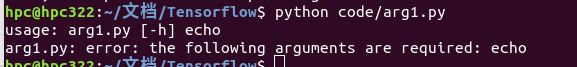
\includegraphics[scale=0.5]{arg1.png}\newline
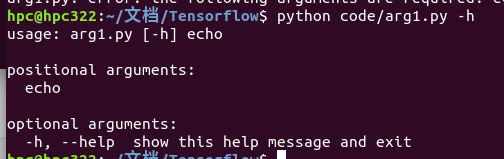
\includegraphics[scale=0.5]{arg2.png}\newline
add\_argument方法指定程序需要接受的命令参数,本例中为echo,此程序运行必须指定一个参数,方法parse\_args()同感分析指定的参数返回数据echo。
\begin{python}
import argparse
parser = argparse.ArgumentParser()
parser.add_argument("echo",help="show the help information",type=int)
args = parser.parse_args()
print(args.echo**2)
\end{python}
指定参数类型为int,默认为string。
\begin{python}
import argparse
parser = argparse.ArgumentParser()
parser.add_argument("--verbosity",help="increase output verbosity")
args = parser.parse_args()
if args.verbosity:
    print("Verbosity turned on")
\end{python}
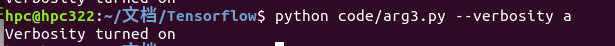
\includegraphics[scale=0.5]{arg3.png}\newline
这里指定了--verbosity程序就显示一些信息,如果不指定程序也不会出错,对应的变量就被设置为None。
\begin{python}
import argparse
parser = argparse.ArgumentParser()
parser.add_argument("--verbosity",help="increase output verbosity",action="store_true")
args = parser.parse_args()
if args.verbosity:
    print("Verbosity turned on")
\end{python}
指定一个新的关键词action,赋值为store\_ture。如果指定了可选参数,args.verbose就赋值为True,否则就为False。
\begin{python}
import argparse
parser = argparse.ArgumentParser()
parser.add_argument("-v","--verbose",help="Increase output verbosity",action="store_true")
args = parser.parse_args()
if args.verbose:
    print("verbosity turned on")
\end{python}
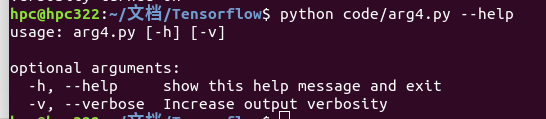
\includegraphics[scale=0.5]{arg4.png}\newline
\begin{python}
#args5.py
import argparse
parser = argparse.ArgumentParser()
parser.add_argument("square",type=int,help="display help information")
parser.add_argument("-v","--verbose",action="store_true",help="increase output verbosity")
args = parser.parse_args()
answer = args.square**2
if args.verbose:
    print("The square of {} equals {}".format(args.square,answer))
else:
    print(answer)
\end{python}
输入参数--verbose和整数(4)顺序不影响结果。
python args5.py --verbose 4和python args5.py 4 --verbose
\begin{python}
import argparse
parser = argparse.ArgumentParser()
parser.add_argument("square",type=int,help="display a square of a given number")
parser.add_argument("-v","--verbosity",type=int,help="increase output verbosity")
args = parser.parse_args()
answer = args.square**2
if args.verbosity == 2:
    print("The square of {} equals {}".format(args.square,answer))
elif args.verbosity == 1:
    print("{}^2=={}".format(args.square,answer))
else:
    print(answer)
\end{python}
python args6.py 4 -v 0,1,2通过指定不同的参数v为0,1,2得到不同的结果。
\begin{python}
#arg7.py
import argparse
parser = argparse.ArgumentParser()
parser.add_argument("square",type=int,help="display the square of a given number")
parser.add_argument("-v","--verbosity",action="count",help="increase output verbosity")
args = parser.parse_args()
answer = args.square**2
if args.verbosity == 2:
    print("The square of {} equals {}".format(args.square,answer))
elif args.verbosity == 1:
    print("{}^2 == {}".format(args.square,answer))
else:
    print(answer)
\end{python}
这里添加参数action="count",统计可选参数出现的次数。
python arg7.py 4 -v(出现一次),对应结果为x\^{}2 == 16\newline
python arg7.py 4 -vv(出现两次),对应出现The square of 4 equals 16\newline
\begin{python}
import argparse
parser = argparse.ArgumentParser()
parser.add_argument("square",type=int,help="display a square of a given number")
parser.add_argument("-v","--verbosity",action="count",default = 0,help="increase output verbosity")
args = parser.parse_args()
answer = args.square**2
if args.verbosity>=2:
    print("The square of {} equals {}".format(args.square,answer))
elif args.verbosity>=1:
    print("{}^2 == {}".format(args.square,answer))
else:
    print(answer)
\end{python}
加速让default参数。这只默认为值0,当参数v不指定时参数就被置为None,None不能和整型比较。
\begin{python}
import argparse
parser = argparse.ArgumentParser()
parser.add_argument("x",type=int,help="The base")
parser.add_argument("y",type=int,help="The exponent")
parser.add_argument("-v","--verbosity",action="count",default=0)
args = parser.parse_args()
answer = args.x**args.y
if args.verbosity >=2:
    print("{} to the power {} equals {}".format(args.x,args.y,answer))
elif args.verbosity >=1:
    print("{}^{} == {}".format(args.x,args.y,answer))
else:
    print(answer)
\end{python}
为了让后面的参数不冲突,我们需要使用另一个方法:
\begin{python}
#args10.py
import argparse
parser = argparse.ArgumentParser()
group = parser.add_mutually_exclusive_group()
parser.add_argument("-v","--verbose",action="store_true")
group.add_argument("-q","--quit",action="store_true")
parser.add_argument("x",type=int,help="The base")
parser.add_argument("y",type=int,help="The exponent")
args = parser.parse_args()
answer = args.x**args.y
if args.quit:
    print(answer)
elif args.verbose:
    print("{} to the power {} equals {}".format(args.x,args.y,answer))
else:
    print("{}^{} == {}".format(args.x,args.y,answer))
\end{python}
可以输入python arg10.py 3 4 -vq得到计算结果。
\begin{python}
import argparse
parser = argparse.ArgumentParser()
group = parser.add_mutually_exclusive_group()
group.add_argument("-v","--verbose",action="store_true")
group.add_argument("-q","--quit",action="store_true")
parser.add_argument("x",type=int,help="The sase")
parser.add_argument("y",type=int,help="The exponent")
args = parser.parse_args()
answer = args.x**args.y
if args.quit:
    print(answer)
elif args.verbose:
    print("{} to the power {} equals {}".format(args.x,args.y,answer))
else:
    print("{}^{} == {}".format(args.x,args.y,answer))
\end{python}
这里参数v和q不能同时使用。


\section{path}
\begin{itemize}
\item os.path.abspath(path):返回path的绝对路径,在多数平台下,相当于调用函数normpath(join(os.getcwd(),path))
\item os.path.basename(path):返回path的路径base name,第二个元素同感传递path给split(),注意这个结果不同于unix的basename程序,这里basename,'foo/bar'然会bar,而basename()函数返回空字符串('')。
\item os.path.commonpath(paths):返回paths队列中最长的sub-path,日国路径中包含绝对路径和相对路径的话将报ValueError或者如果paths是空,不想commonprefix(),这个函数返回一个错的路径。
\item os.path.dirname(path):返回目录的名字,就是path用split分割厚的第一个元素。
\item os.path.exists(path):如果春在路径path或者一个打开的文件描述返回True。对于破掉的符号链接返回False,在一些平台,如果权限不允许执行os.stat()即使存在物理路径这个函数也返回False。
\item os.path.lexists(path):如果路径存在返回True,对broken 符号链接返回True,等效与exists()。
\item os.path.expanduser(path):在Unix和Windows上用~或者~user取代用户路径的值。在unix上一个~被环境变量HOME替代(如果设置了HOME环境变量的话),否则当前用户的home目录通过内建模块pwd查找,一个初始化~user是寻找在password目录里面的目录。\item os.expandvars(path):返回环境变量的值,子字符串形式时${name}或者$name被环境变量名取代,变形的变量名字和参考不存在的变量将不改变。
\item os.path.getatime(path):返回上次访问路径的时间,返回一个从epoch起经历的秒数,如果文件不存在或不可访问则报OSError。
\item os.path.getmtime(path):返回最新修改路径的时间,返回值时一个epoch其开始的秒数,文件不存在或者不可范围跟时报OSError。
\item os.path.getctime:返回系统的ctime,在Unix上时最新的metadata改变的时间,在windows上时path创建的时间,返回一个从epoch起经历的秒数,如果文件不存在或不可访问则报OSError。
\item os.path.getsize(path):返回字节表示的路径的大小,如果不存在文件或者文件不可范围跟将报出OSError。
\item os.path.isabs(path):如果路径是绝对路径返回True。
\item os.path.isfile(path):如果路径是文件将返回True。
\item os.path.isdir(path):如果存在路径返回True。
\item os.path.islink(path):如果路径查询一个目录入口时符号链接返回True,如果Python运行时符号链接不支持将返回False。
\item os.path.ismount(path):如果path是一个挂载点,返回True。
\item os.path.join(path,*paths):加入一个或者更多的组建,返回值是连接路径和任何成员的路径。
\item os.path.normcase(path):在Unix,MAX OS上返回路径不变,在一些敏感的文件系统上将转换路径为小写,在windows上将转化斜线为饭斜线,如果path不是str或者bytes将报TypeError。
\item os.path.normpath(path):删除冗余得分和服,因此A//B,A/B,A/./B,A/foo../B将变为A/B.字符串操作也许改变包含符号链接的意义,在windows上它转化斜线为反斜线。
\item os.path.realpath(path):返回指定文件名的确定路径,消除路径中出现的任何符号链接。
\item os.realpath(path,start=os.curdir):从当前路径或者start路径返回相对的文件路径,这是一个路径计算:文件系统不妨问确定的存在的或者自然的路径或者start。
\item os.path.samefile(path1,path2):如果pathname值访问相同的文件或者目录则返回True,这有device名字和i-node数量决定,如果os.stat()调用pathname失败将报出异常。
\item os.path.sameopenfile(fp1,fp2):如果fp1和fp2指定的时相同的文件将返回True。
\item os.path.samestat(stat1,stat2):如果元组stat1和state2查询的时相同的文件,返回True,这个结构可需已经被os.fstate(),os.lstat()或者os.stat()返回,番薯通过samefile()和sameopenfile()实现基本的比较。
\item os.path.split(path):分割路径为(head,tail)。tail不包含斜线,如果以斜线将诶为,tail将为空,如果没有斜线,头将为空,如果path时空,头尾都为空。后面的斜线从head删除出位它是root(一个或者更多的斜线),在所有的情况下join(head,tail)返回一个路径到相同位置作为路径。

\item os.path.splitdrive(path):返回pathname到(drive,tail),这里drive可以使挂载点或者空字符串。在系统上没有用驱动器指定,驱动器将为空字符串,在所有的倾向下,drive+tail将时相同的路径。在Windows上,分割pathname成drive/UNC共享点和相对路径,如果路径包含驱动器驱动器将包含冒号(splitdrive("c:/dir"))返回("c:","/dir"),如果路径包含驱动UNC路径,驱动器将包含主机名和share,但是不包含四个分隔符splitdrive("//host/computer/dir")return("//host/computer","/dir")
\item os.path.split(path):分割路径名为(root,ext)像root+ext == path,ext时空或者以一个周期开头,导致basename被忽略,splitex('.cshrc')返回('.cshrc','')
\item os.path.supports\_unicode\_filenames():如果文件名时unicode编码的则为True。
\end{itemize}

\chapter{Tensorflow API}
\section{tf.app.flags}
\subsection{DEFINE\_boolean}
DEFINE\_boolean(flag\_name,default\_value,docstring):定义一个'boolean'类型的flag。
\begin{itemize}
\item flag\_name:flag的名字,是一个字符串。
\item default\_value:flag应被被看作一个boolean的默认值。
\item docstring:用flag的一个帮助信息。
\end{itemize}
\subsection{DEFINE\_boolean}:定义一个'boolean'类型的flag。
\begin{itemize}
\item flag\_name:flag的名字,是一个字符串。
\item flag\_default\_value:默认的boolean类型的值。
\item docstring:用flag的一个有用的帮助信息。
\end{itemize}
\subsection{DEFINE\_float}:定义一个浮点数类型的flag。
\begin{itemize}
\item flag\_name:作为flag的名字,应该是字符串。
\item default\_value:flag的默认值,应该是浮点数。
\item docstring:用flag的一个有用的帮助信息。
\end{itemize}
\subsection{DEFINE\_integer}:定义一个整数的flag。
\begin{itemize}
\item flag\_name:flag的名字,应该是字符串。
\item default\_value:flag的默认值,应该是一个整数。
\item docstring:用flag的一个有用的帮助信息。
\end{itemize}
\subsection{DEFINE\_string}:定义一个字符串的flag。
\begin{itemize}
\item flag的名字,应该是字符串。
\item default\_value:flag的默认值,应该是字符串。
\item docstring:用flag的一个有用的帮助信息。
\end{itemize}
\subsection{tf.gather}
\begin{python}
gather(
    params,
    indices,
    validate_indices=None,
    name=None,
    axis=0
	)
\end{python}
根据indices从params和axis轴获取slices。
indices必须是任何维度(通常是0维或者一维)的一个整数tensor生成输出tensor的形状params.shape[:axis]+indices.shape+params.shape[axis+1:],这里
\begin{python}
# Scalar indices (output is rank(params) - 1).
output[a_0, ..., a_n, b_0, ..., b_n] =
params[a_0, ..., a_n, indices, b_0, ..., b_n]
# Vector indices (output is rank(params)).
output[a_0, ..., a_n, i, b_0, ..., b_n] =
params[a_0, ..., a_n, indices[i], b_0, ..., b_n]
# Higher rank indices (output is rank(params) + rank(indices) - 1).
output[a_0, ..., a_n, i, ..., j, b_0, ... b_n] =
params[a_0, ..., a_n, indices[i, ..., j], b_0, ..., b_n]
\end{python}
\begin{figure}[H]
	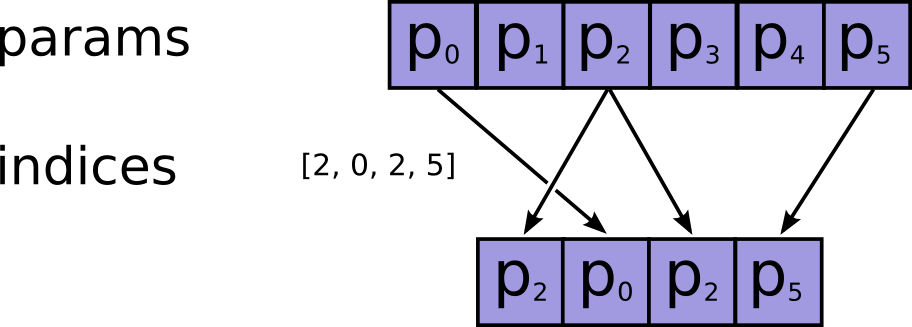
\includegraphics[scale=0.5]{Gather.png}
\end{figure}
参数:
\begin{itemize}
	\item params:一个Tensor,从它那里收集值,rank必须是axis+1
	\item indices:一个tensor。必须是int32,int64.索引tensor,必须是在[0,params.shape[axis])
	\item axis:一个Tensor,必须是下面的数据类型:int32,int64.params的轴,从params中获得收集索引,默认是第一维,支持负索引。
	\item name:操作的名字
	\item{返回}:一个tensor,和params有相同的数据类型,通过给定indeces从params收集,形状为[params.shape[:axis]+indices.shape+params.shape[axis+1:]
\end{itemize}
例子:
\begin{python}
import tensorflow as tf
a = tf.constant([[1,2,3,4],[5,6,7,8],[9,10,11,12],[13,14,15,16]])
b = tf.constant([1,0,2])
g = tf.gather(a,b)
with tf.Session() as sess:
    print(sess.run(g))#获取第一轴[1,0,2]行的数据
\end{python}
输出:
\begin{python}
[[ 5  6  7  8]
 [ 1  2  3  4]
 [ 9 10 11 12]]
\end{python}
\subsection{tf.placeholder}
\begin{python}
placeholder(
    dtype,
    shape=None,
    name=None
)
\end{python}
为placeholder输入需要被插入的tensor。
如果这个tensor被计算将产生错误。他的值必须通过feed\_dict选项在Session.run(),Tensor.eval()或者是Operation.eval()输入。
\begin{python}
x = tf.placeholder(tf.float32, shape=(1024, 1024))
y = tf.matmul(x, x)
with tf.Session() as sess:
    print(sess.run(y))  # ERROR: will fail because x was not fed.
    rand_array = np.random.rand(1024, 1024)
    print(sess.run(y, feed_dict={x: rand_array}))  # Will succeed.
\end{python}
参数:
\begin{itemize}
\item dtype:被输入的tensor元素的数据类型。
\item shape:被fed的tensor的形状,如果形状没有被指定,你可以输入任何形状的tensor。
\item:操作的名字
\item{Return} 一个可能被用作输入数据处理的Tensor,值不能被直接计算。
\end{itemize}
\subsection{tf.squeeze}
tf.squeeze(input,axis=None,name=None,squeeze\_dims=None)
说明:从指定的Tensor中移除1维度。
\begin{itemize}
\item input:tensor,输入Tensor。
\item axis:列表,指定需要移除的位置的列表,默认为空列表[],索引从0开始squeeze不为1的索引会报错。
\item name:操作的名字
\item squeeze\_dims:否决当前轴的参数。
\item 返回一个Tensor,形状和input相同,包含和input相同的数据,但是不包含有1的元素。
\item 异常:squeeze\_dims和axis同时指定时会有ValueError。
\end{itemize}
\# 't' is a tensor of shape [1, 2, 1, 3, 1, 1]\newline
shape(squeeze(t)) ==> [2, 3]\newline
\# 't' is a tensor of shape [1, 2, 1, 3, 1, 1]\newline
shape(squeeze(t, [2, 4])) ==> [1, 2, 3, 1]\newline
\subsection{tf.metrics}
accuracy(labels,predictions,weights=none,metrics\_collections,updates\_collections=none,name=none)
\begin{itemize}
	\item labels:tensor,和predictions的形状相同,代表真实值。
	\item predictions:tensor,代表预测值。
	\item weights:tensor,rank可以为0或者labels的rank,必须能和label广播(所有的维度必须是1,或者和labels维度相同)
	\item metrics\_collection:accuracy应该被增加的一个collectiobn列表选项。
	\item update\_collections:update\_op应该添加的选项列表。
	\item name:variable\_scope名字选项。
	\item accuracy:返回值tensor,代表精度,总共预测对的和总数的商。
	\item update\_op:返回值适当增加total和count变量和accuracy匹配。
	\item valueerror:异常如果predictions和labels有不同的形状,或者weight不是none它的形状不合prediction匹配,或者metrics\_collections会哦这updates\_collections不是一个list或者tuple。
\end{itemize}

\subsection{tf.stack}
stack(values,axis=0,name='stack'):stack一个n维tensor为n+1维tensor。
给定一个长度为N的形状为(A,B,C)的tensor,如果axis==0输出tensor的形状为(N,A,B,C),如果axis==1,输出tensor的形状为(A,N,B,C)
\# 'x' is [1,4]\newline
\# 'y' is [3,6]\newline
\# 'z' is [3,6]\newline
stack([x,y,z])==>[[1,4],[2,5],[3,6]]\newline
stack(x,y,z,axis=1)==>[[1,2,3],[4,5,6]]\newline
tf.stack([x,y,z]) = np.asarray([x,y,z])\newline
输出参数:
\begin{itemize}
	\item 一个Tensor列表。
	\item 整数,默认为0,支持负坐标。
	\item 操作的名字。
	\item[\S] 一个stack的Tensor。
	\item[\S] ValueError:如果axis超过[-(R+1),R+1)
\end{itemize}
\textsl{Example}
\begin{python}
import tensorflow as tf
x = tf.constant([1,4])
y = tf.constant([2,5])
z = tf.constant([3,6])
r1 = tf.stack([x,y,z])
r2 = tf.stack([x,y,z],axis=1)
with tf.Session() as sess:
    print(sess.run(r1).shape)
    print(sess.run(r2).shape)
\end{python}
\subsection{tf.reshape}
tf.reshape(tensor,shape,name=None)
\begin{itemize}
	\item Tensor:一个Tensor。
	\item shape:一个列表,数值类型为int32或者时int64
	\item name:操作的名字。
	\item[S] 指定形状的Tensor。
\end{itemize}
\begin{python}
import tensorflow as tf
a = tf.linspace(0.,9.,10)
b = tf.reshape(a,[2,5])
with tf.Session() as sess:
    a = sess.run(a)
    b = sess.run(b)
print(a.shape)
print(b.shape)
\end{python}
\subsection{tf.random\_crop}
\begin{python}
random_crop(
    value,
    size,
    seed=None,
    name=None
)
\end{python}
从value tensor随机剪裁一块指定size的tensor,要求value。shape大于参数size的值。如果一维不剪切需要传递完整的size,例如RGB图像可以用size = [crop\_height,crop\_width,3]剪切。

输入参数:
\begin{itemize}
\item value:需要被剪切的tensor
\item size:和value有相同rank的一维tensor。
\item seed:Python整数,用于创建一个随机种子。
\item name:操作的名字。
\item[Retuen] 一个剪切的和value有相同的rank,形状为size的tensor。
\end{itemize}
\subsection{tf.random\_gamma}
\begin{python}
random_gamma(
    shape,
    alpha,
    beta=None,
    dtype=tf.float32,
    seed=None,
    name=None
)
\end{python}
从指定\href{https://zh.wikipedia.org/wiki/伽玛分布}{Gamma分布}中获得shape样本,alpha是形状参数,beta是反向放大参数。

输入参数:
\begin{itemize}
\item shape:一个一维整数Tensor或者Python数组,指定alpha,beta参数的输出采样数据。
\item alpha:一个tensor或者python值或者N维dtype数据类型。alpha提供形状参数,必须和beta广播。
\item beta:一个tensor或python值或者dtype类型的n维数组。默认为1.beta提供gamma分布的反向放大参数。必须和alpha广播。
\item dtype:alpha,beta,output的输出:float16,float32或者float64。
\item seed:一个Python整数,用于创建随机种子。
\item name:操作的选项。
\item[Returns]:
samples:数据类型为dtype的一个形状为tf.concat(shape,tf.shape(alpha+beta))的tensor。
\end{itemize}
例子:
\begin{python}
samples = tf.random_gamma([10],[0.5,1.5])#形状为10,alpha为0.5,1.5,采样输出形状为[10,2]
samples = tf.random_gamma([7, 5], [0.5, 1.5]) # 采样输出形状为[7, 5, 2], where each slice [:, :, 0] and [:, :, 1] # 代表从两个分布采样的$7\items5$。
samples = tf.random_gamma([30], [[1.],[3.],[5.]], beta=[[3., 4.]]) #采样输出形状[30, 3, 2], 每$2\times2$(广播运算)30个采样点
\end{python}
\subsection{tf.random\_normal}
\begin{python}
random_normal(
    shape,
    mean=0.0,
    stddev=1.0,
    dtype=tf.float32,
    seed=None,
    name=None
)
\end{python}
输出正态分布随机值。

输入参数:
\begin{itemize}
\item shape:一个一维整数tensor或者Python数组。表示输出tensor的形状。
\item mean:一个0维tensor和dtype的Python值,正态分布的均值。
\item stddev:一个0维tensor和dtype的Python值,正态分布的标准差。
\item stype:输出数据类型。
\item seed:一个整数,用于创建一个随机数种子。
\item name:操作的名字。
\item[Returns] 制订形状的正态分布值。
\end{itemize}
\subsection{\textbf{tf.random\_normal\_initializer}}
继承于\href{https://www.tensorflow.org/api_docs/python/tf/contrib/keras/initializers/Initializer}{Initializer}
别名:
\begin{itemize}
\item Class tf.contrib.keras.initializers.RandomNormal
\item Class tf.random\_normal\_initializer
\end{itemize}
输入参数:
\begin{itemize}
\item mean:一个python标量或者标量tensor。生成随机值的均值。
\item stddev:一个python标量或者标量tensor。标生成随机值的标准差。
\item seed:python整数,用于创建随机种子。
\item dtypes:数据类型,仅仅支持浮点数类型。
\end{itemize}
方法:
\begin{itemize}
\item \_\_init\_\_
\begin{python}
__init__(
    mean=0.0,
    stddev=1.0,
    seed=None,
    dtype=tf.float32
)
\end{python}
\item \_\_call\_\_
\begin{python}
__call__(
    shape,
    dtype=None,
    partition_info=None
)
\end{python}
\item from\_config:从配置字典实例化initilizer。
\begin{python}
from_config(
    cls,
    config
)
\end{python}
例如:
\begin{python}
initializer = RandomUniform(-1, 1)
config = initializer.get_config()
initializer = RandomUniform.from_config(config)
\end{python}
\item get\_config()
\end{itemize}
\subsection{tf.random\_possion}
\begin{python}
random_poisson(
    lam,
    shape,
    dtype=tf.float32,
    seed=None,
    name=None
)
\end{python}
从Poisson分布中获取制定形状的样本,lam是描述分布的参数。

输入参数:
\begin{itemize}
\item lam:一个Tensor或者Python值或者dtype指定的N维数组。lam是Poisson分布的参数。
\item shape:yuige一维整数tensor或者python数组,输出每个rate指定的参数的形状。
\item dtype:lam和输出的数据类型:float16,float32,float64.
\item seed:Python整数,用于创建一个分布的随机种子。
\item name:操作的名字。
\item[Returns]:形状为tf.concat(shape,tf,shape(lam))的tensor(值的数据类型如dtype指定)。
\end{itemize}
例子:
\begin{python}
samples = tf.random_poisson([0.5, 1.5], [10]) # 采样输出形状为[10, 2],切片输出 [:, 0] and [:, 1] 代表不同分布的数据

samples = tf.random_poisson([12.2, 3.3], [7, 5]) # 采样输出形状[7, 5, 2], chide切片[:, :, 0]和[:, :, 1]代表 $7\times5$从两个分布的采样输出。
\end{python}
\subsection{random\_shuffle}
\begin{python}
random_shuffle(
    value,
    seed=None,
    name=None
)
\end{python}
沿着tensor的一维随机打乱数据。像value[j]映射一个tensor到一个数出output[i]。例如
\begin{python}
[[1, 2],       [[5, 6],
 [3, 4],  ==>   [1, 2],
 [5, 6]]        [3, 4]]
\end{python}
输入参数:
\begin{itemize}
\item value:一个应该被打乱的值。
\item seed:一个python正数用于创建随机数种子。
\item name:操作的名字。
\item[Returns] 一个指定类型的值和形状,沿着某一维读被打乱的tensor。
\end{itemize}
\subsection{tf.random\_uniform}
\begin{python}
random_uniform(
    shape,
    minval=0,
    maxval=None,
    dtype=tf.float32,
    seed=None,
    name=None
)
\end{python}
输出均匀分布的随机值,生成的值的范围在[minival,maxval),下界minval包含在范围内,上界不再。对于浮点数默认范围是[0,1)。至少maxval必须被明确指定。在整数情况下,会有一些轻微的偏移,除非maxval-minval是2的次幂。偏移是maxval-minval
比较小的值相对于输出范围(2**32,2**64)很小。

输入参数:
\begin{itemize}
\item shape:一维整数tensor或者Python数组,和数出tensor的形状相同。
\item minval:0维tensor或者dtype指定的python值,生成随机数的下界,默认为0,。
\item maxval:0维tensor或者dtype指定的python值。生成随机数的上界,dtype是浮点数时,默认为1。
\item dtype:输出的类型:'float16,float32,float64,int32,int64'。
\item seed:一个Python整数。用于创建分布的随机数种子。
\item 操作的名字。
\item [Return] 返回指定形状的均匀分布值。
\item [Raise] ValueError:如果dtype是整数并且maxval没有被指定。
\end{itemize}
\subsection{\textbf{tf.random\_uniform\_initializer}}
一个继承自Initilizer的类。

别名:
\begin{itemize}
\item tf.contrib.keras.initializers.RandomUniform
\item tf.random\_uniform\_initializer
\end{itemize}
生成均匀分布tensor的initializer。

输入参数:
\begin{itemize}
\item minval:0维tensor或者dtype指定的python值,生成随机数的下界,默认为0,。
\item maxval:0维tensor或者dtype指定的python值。生成随机数的上界,dtype是浮点数时,默认为1。
\item seed:一个Python整数。用于创建分布的随机数种子。
\item dtype:输出的类型:'float16,float32,float64,int32,int64'。
\end{itemize}
方法:
\begin{itemize}
\item \begin{python}__init__(
    minval=0,
    maxval=None,
    seed=None,
    dtype=tf.float32
)\end{python}
\item \_\_call\_\_
\begin{python}
__call__(
    shape,
    dtype=None,
    partition_info=None
)
\end{python}
\item from\_config
\begin{python}
from_config

from_config(
    cls,
    config
)
\end{python}
\item get\_config
\end{itemize}
\subsection{tf.one\_hot}
\begin{python}
ne_hot(
    indices,
    depth,
    on_value=None,
    off_value=None,
    axis=None,
    dtype=None,
    name=None
)
\end{python}
返回一个One-hot tensor。
indices表示的下表的值为on\_value,所有其它值为off\_value。

如果on\_value不提供,默认为dtype下的1。off\_value不提供,默认值为0,如果输入Incices rank是N,输出rank将是N+1。新的axis将在axis创建。,如果indices是一个标量,输出形状将是一个depth长度的向量,如果indices是亿个长度为features向量输出形状将为:
\begin{python}
feature x depth ifn axis == -1
depth x features if axis == 0
\end{python}
如果indices是一个矩阵,形状为[batch,features],输出形状将为:
\begin{python}
 batch x features x depth if axis == -1
  batch x depth x features if axis == 1
  depth x batch x features if axis == 0
\end{python}
如果dtype没有被提供,他将假设on\_value或off\_value的数据类型,如果一个或者倍多的值呗传递,,如果没有on\_value,off\_value,或者dtype被提供,dtype将默认tf.float32。
例子:

假设:
\begin{python}
indices = [0, 2, -1, 1]
  depth = 3
  on_value = 5.0
  off_value = 0.0
  axis = -1
\end{python}
输出形状为[$4\times3$]
输出:
\begin{python}
output =
  [5.0 0.0 0.0]  // one_hot(0)
  [0.0 0.0 5.0]  // one_hot(2)
  [0.0 0.0 0.0]  // one_hot(-1)
  [0.0 5.0 0.0]  // one_hot(1)
\end{python}
假设:
\begin{python}
 indices = [[0, 2], [1, -1]]
  depth = 3
  on_value = 1.0
  off_value = 0.0
  axis = -1

\end{python}
输出
\begin{python}
output =
  [
    [1.0, 0.0, 0.0]  // one_hot(0)
    [0.0, 0.0, 1.0]  // one_hot(2)
  ][
    [0.0, 1.0, 0.0]  // one_hot(1)
    [0.0, 0.0, 0.0]  // one_hot(-1)
  ]
\end{python}
用默认on\_value和off\_value:
\begin{python}
indices = [0, 1, 2]
  depth = 3
\end{python}
输出
\begin{python}
  output =
  [[1., 0., 0.],
   [0., 1., 0.],
   [0., 0., 1.]]
\end{python}
参数:
\begin{itemize}
\item indices:一个索引的Tensor。
\item depth:一个定义one hot维度的深度的标量。
\item on\_vlaue:制定Indices[j]=i(填入i),默认为1。
\item off\_value:一个标量当Indices[j]!=i(默认为0)。
\item axis:填入的轴,默认为-1。
\item dtype:输出tensor的数据类型。
\item [Returns]:one-hot tensor。
\item [Raise]
\begin{itemize}
\item TypeError:如果dtype和on\_value,off\_value数据类型不一样。
\item TypeError:如果on\_value和off\_value不合另一个匹配。
\end{itemize}
\end{itemize}
\subsection{tf.unstack}
\begin{python}
unstack(
    value,
    num=None,
    axis=0,
    name='unstack'
)
\end{python}
unstack rank-R为rank-(R-1)的tensor。通过chipping沿着axis从value unstack num tensor。如果num不被指定(默认)它从value的形状推算。如果value.shape[axis]不知道,ValueError异常。
例如一个tensor的形状为(A,B<C<D);
如果 axis ==0输出第i维的切片value[i,:,:,:],output的输出每个tensor形状为(B,C,D).(注意沿着维度unstack)
如果axis == 1然后输出第i个tensor在切片的值[:,i,:,:]和每个output的每个输出将有形状(A,C,D)。
tf.ustack(x,n)=list(x)

参数:
\begin{itemize}
\item value:rank R>0的Tensor能被unstack。
\item num 一个整数。axis的长度,如果为None将自动推断。
\item axis:一个整数。ustack沿着的轴。默认是第一维,支持负的索引。
\item name:操作的名字。
\item[Returns] 从value unstack的Tensor列表。
\item[Raises]:
\begin{itemize}
\item ValueError:如果num没有被指定且不能推断出。
\item ValueError:如果axis超过[-R,R)。
\end{itemize}
\end{itemize}

\section{tf.image}
\subsection{tf.image.decode\_gif}
tf.image.decode\_gif(contents,name=None)
\begin{itemize}
\item contents:一个字符串Tensor,GIF编码的图像。
\item name:操作的名字。
\item 返回一个8位无符号的Tensor,四维形状为[num\_frames,height,width,3],通道顺序是RGB。
\end{itemize}
\subsection{tf.image.decode\_jpeg}
tf.image.decode\_jpeg(contents,channels=None,ratio=None,fancy\_upscaling=None,\newline
try\_recover\_truncated=None,acceptable\_fraction=None,dct\_metched=None,name=None)
解码JPEG编码的图像为无符号的8位整型tensor。\newline
\begin{itemize}
	\item contents:一个字符串tensor,JPEG编码的图像。
	\item channels:一个整数默认为,0代表编码图像的通道数(JPEG编码的图像),1代表灰度图,3带秒RGB图。
	\item radio:一个整数,默认为1,取值可以是1,2,4,8,表示缩减图像的比例。
	\item fancy\_upscaling:bool型,默认为True,表示用慢但是更好的提高色彩浓度。
	\item try\_recover\_truncated:bool型,默认是False,如果时True尝试从截断的输入恢复图像。
	\item acceptable\_fraction:float型,默认是1,可接受的最小的截断输入的因子。
	\item dct\_methed:string类型,默认为"".指定一个解压算法,默认是""由系统自行指定。可用的值有["INTEGER\_FAST","INTEGER\_ACCURATE"]
	\item name:操作的名字。
	\item 返回值为一个8位无符号整型Tensor,3维形状[height,width,channels]
\end{itemize}
\subsection{tf.image.encode\_jpeg}
tf.image.encode\_jpeg(image,format=None,quality=None,progressive=None,optimize\_size=None\newline
chroma\_downsampling=None,density\_uint=None,x\_density=None,y\_density=None,xmp\_metadata=None,name=None)
\begin{itemize}
	\item image:一个3维[height,width,chennels],8位无符号整型Tensor。
	\item format:string类型,可以为"","grayscale","rgb",默认为""。如果format没有指定或者不为空字符串,默认格式从image的通道中选,1:输出灰度图,3:输出RGB图。
	\item quality:整型,默认值为95,代表压缩质量值[0,100],值越大越好,单速度越慢。
	\item optimize\_size:bool型,默认为False,如果为True用CPU/RAM减少尺寸同时保证质量。
	\item chroma\_downsampling:bool型,默认为True。
	\item density\_unit:一个字符串,可以为"in","cm",指定x\_density和y\_density.in每inch的像素,cm表示每厘米的像素。
	\item x\_density:一个整数,默认为300,每个density单位的水平像素。
	\item y\_density:一个整数,默认为6300,数值方向上每density单位的像素。
	\item xmp\_metadata:string类型,默认为"",如果为空,嵌入XMP metadata到图像头部。
	\item name:操作的名字。
	\item name:操作的名字。
	\item 返回0维字符串型JPED编码的Tensor。
\end{itemize}
\subsection{tf.image.decode\_png}
tf.image.decode\_png(contents,channels=None,dtype=None,name=None)
解码PNG编码的图像为8位或者16位无符号整型Tensor。
\begin{itemize}
	\item contents:一个0维PNG编码的图像的字符串的Tensor。
	\item chennels:整型默认为0,代表解码图像的通道,0用PNG编码图像数,1:代表输出灰度图像。3:代表输出RBG图像。4:输出RGBA图像。
	\item dtype:tf.DType,值可以为tf.uint8,tf.uint16,默认为tf.uint8。
	\item name:操作的名字。
	\item 返回3维[height,width,channels]的Tensor。

\end{itemize}
\subsection{tf.image.encode\_png}
tf.image.encode\_png(image,compression=None,name=None)
\begin{itemize}
	\item 一个8位或者16位的3维Tensor,形状为[height,width,channels]
	\item compression:一个整数,默认为-1,表示压缩等级。
	\item name:操作的名字。
	\item 返回一个0维string型的PNG-encoded的Tensor。
\end{itemize}
\subsection{tf.image.decode\_image}
tf.image.decode\_image(contents,channels=None,name=None)
\begin{itemize}
	\item contens:0维编码图像的字符串。
	\item channels:整数,默认为0,解码图像的通道数。
	\item name:操作的名字。
	\item 返回JPEG,PNG的8位无符号的形状为[height,width,num\_channels],GIF文件的形状为[num\_frames,height,width,3]
	\item ValueError:通道数不正确。
\end{itemize}
\subsection{tf.image.resize\_images}
tf.image.resize\_images(images,size,method=ResizeMethed.BILINEAR,align\_corners=False)
\begin{itemize}
	\item images:形状为[batch,height,width,channels]4维Tensor,3为Tensor,形状为[height,width,channels]
	\item size:一位32整型Tensor元素为new\_height,new\_width,新的图像尺寸。
	\item methed:ResizeMethod,默认为ResizeMethod.BILINEAR
		\begin{itemize}
			\item ResizeMethod.BILINEAR:二进制插值。
			\item ResizeMethod.NEAGREST\_NEIGHBOR:
			\item ResizeMethod.BICUBIC:
			\item ResizeMethod.AREA:
		\end{itemize}
	\item align\_corners:bool型,如果为真提取对齐四个角,默认为False。
	\item 异常
		\begin{itemize}
			\item ValueError:图像形状和函数要求的不一样。
			\item ValueError:size是不可以用的形状或者类型。
			\item ValueError:指定的方法不支持。
		\end{itemize}
	\item 如果图像时4维[batch,new\_height,new\_height,channels],如果图像是3维,形状为[new\_height,new\_width,channels]
\end{itemize}

\end{document}
